\documentclass[../document.tex]{subfiles}
\begin{document}
\chapter{Implementation}
\label{chap: implementation}
This section talks in detail about the implementation of the framework. We will first talk about from the utilized robot, then describe each step in the dataset generation, illustrate the utilized estimators and finish by listing the employed software.
\section{Robot}
We tested our framewotk on a a legged crocodile-like robot called \emph{Krock} developed at \href{https://biorob.epfl.ch/}{EPFL}. The next figure shows the robot in real life with a cloat and in a simulated enviroment.

\begin{figure}[htbp]
    \centering
         \begin{subfigure}[b]{0.45\textwidth}
        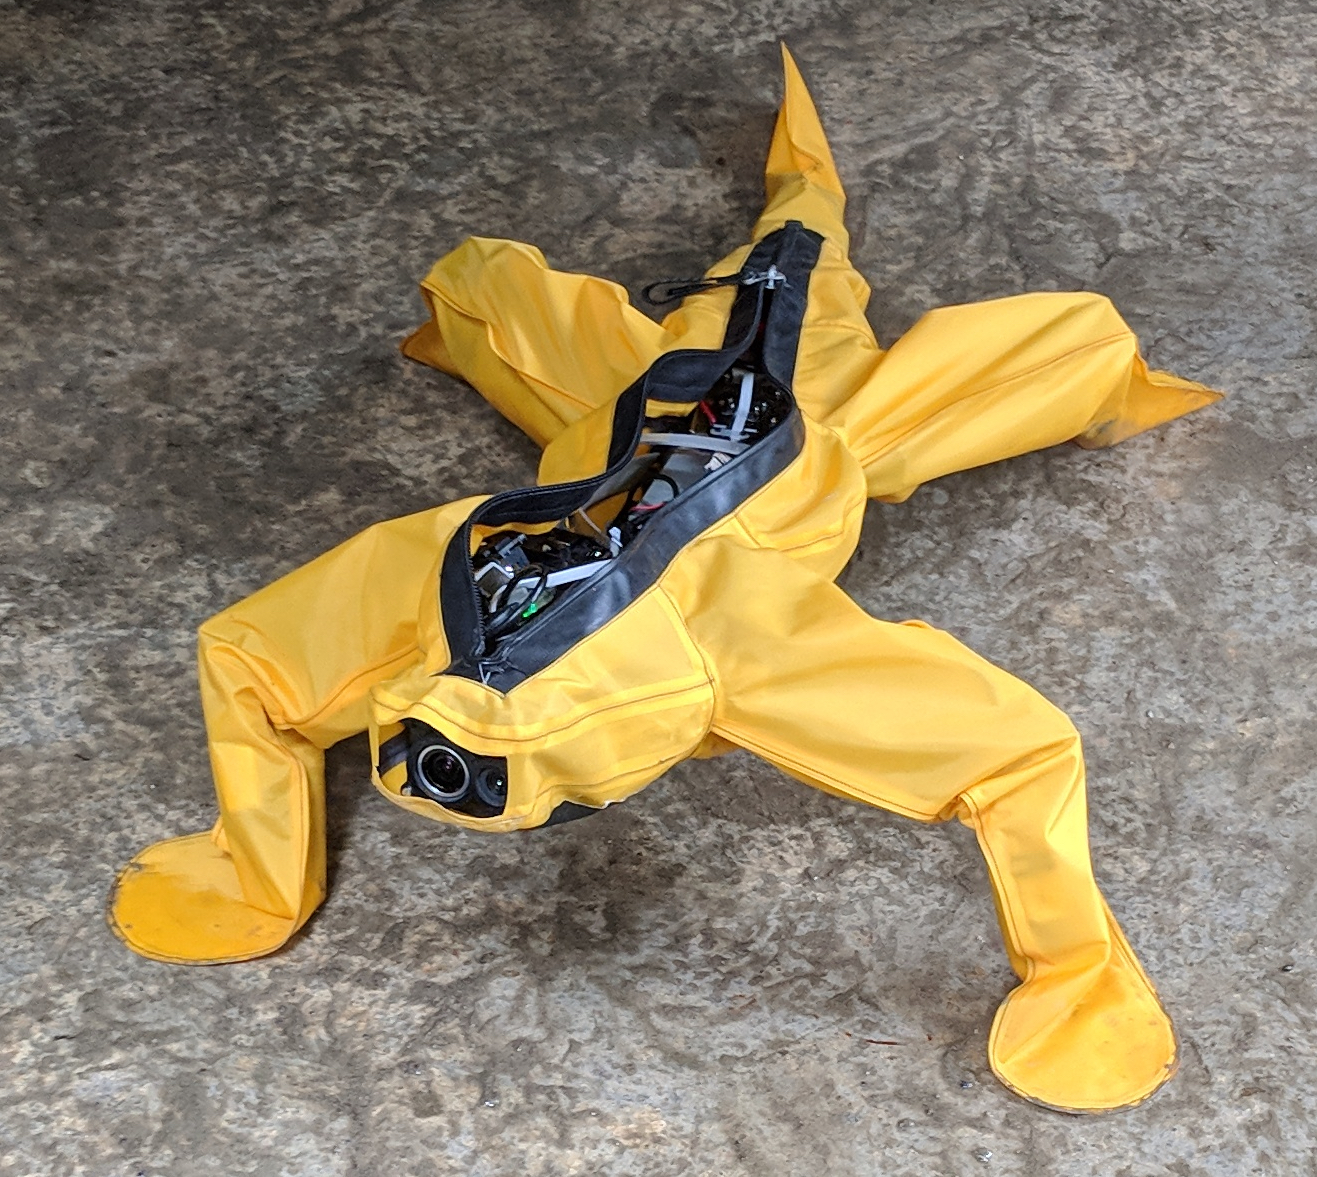
\includegraphics[width=\textwidth]{../img/krock-real.jpg}
        \caption{Krock in real life.}
    \end{subfigure}
         \begin{subfigure}[b]{0.45\textwidth}
          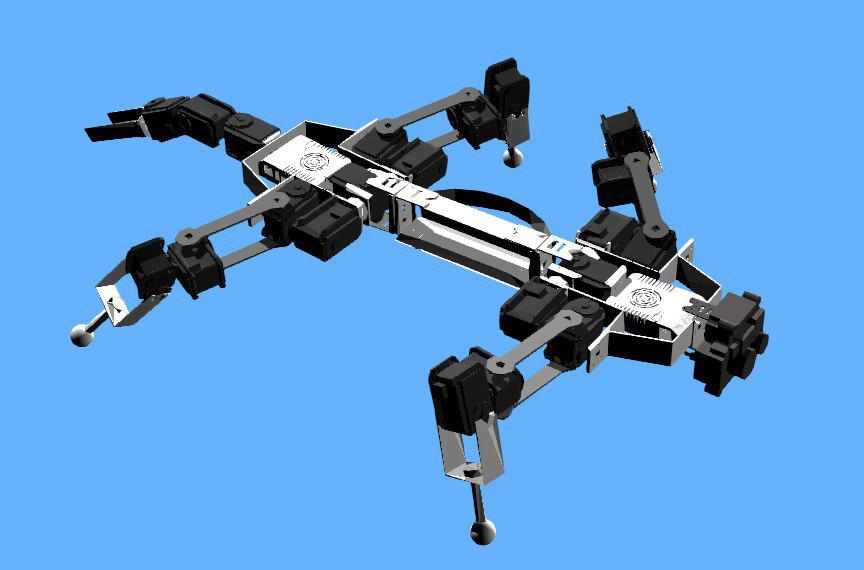
\includegraphics[width=\textwidth]{../img/krock-1.jpg}
          \caption{Krock in the simulator.}
        \end{subfigure}
           \caption{\emph{Krock}}
           \label{fig: krock}

    \end{figure}
    Krock robot was created for the porpuse of montoring real crocodiles, hence it must walk and behave realistically enough to fool the real crocodiles. Krock has four legs, each one of them is equipped with three motors in order to rotate in each axis. The robot can raise itself in three different configurations, gaits, using the four motors on the body connected to the legs. In addition, there are another set of two motors in the inner body part to increase Krock's move set. 
The tail is composed by another set of three motors and can be used to perform a wide array of tasks.
The robot is $85cm$ long, weights around $1.4kg$ and in its standard gait configuration its distance from the ground is $16$cm. The next figure \ref{fig:krock-top} shows \emph{Krock} from the top helping the reader understanding its composition and the correct ratio between its parts. Also, each motor is highlighted with a red marker.
\begin{figure}[htbp]
\centering
     \begin{subfigure}[b]{0.49\textwidth}
    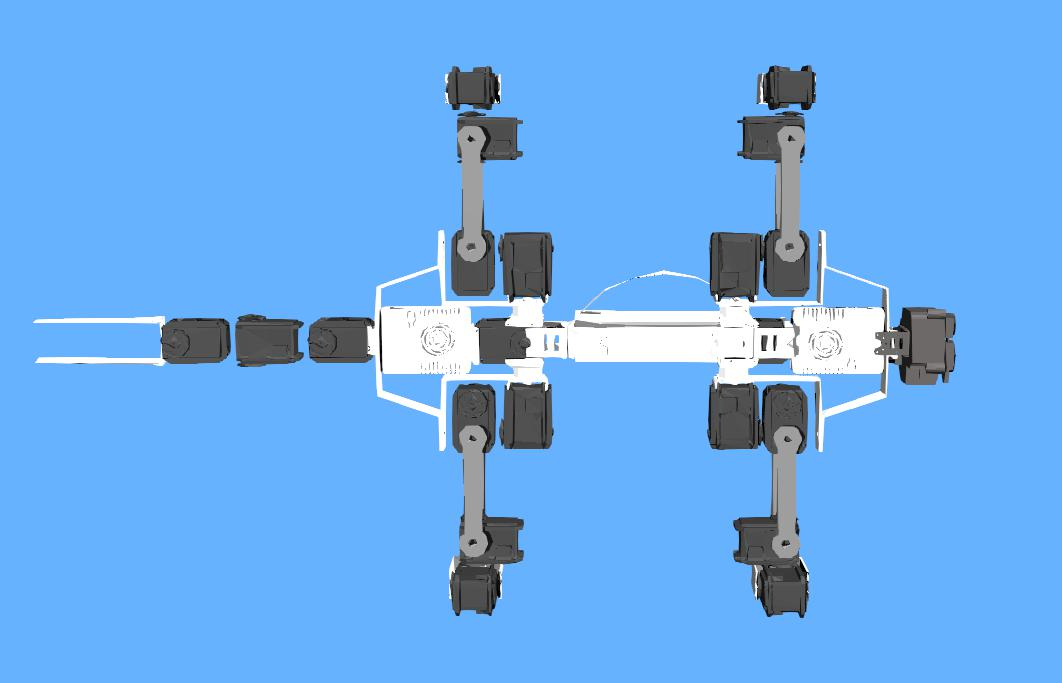
\includegraphics[width=\textwidth]{../img/krock-top.jpg}
    \caption{Top view of \emph{Krock}}
   	\end{subfigure}
     \begin{subfigure}[b]{0.49\textwidth}
      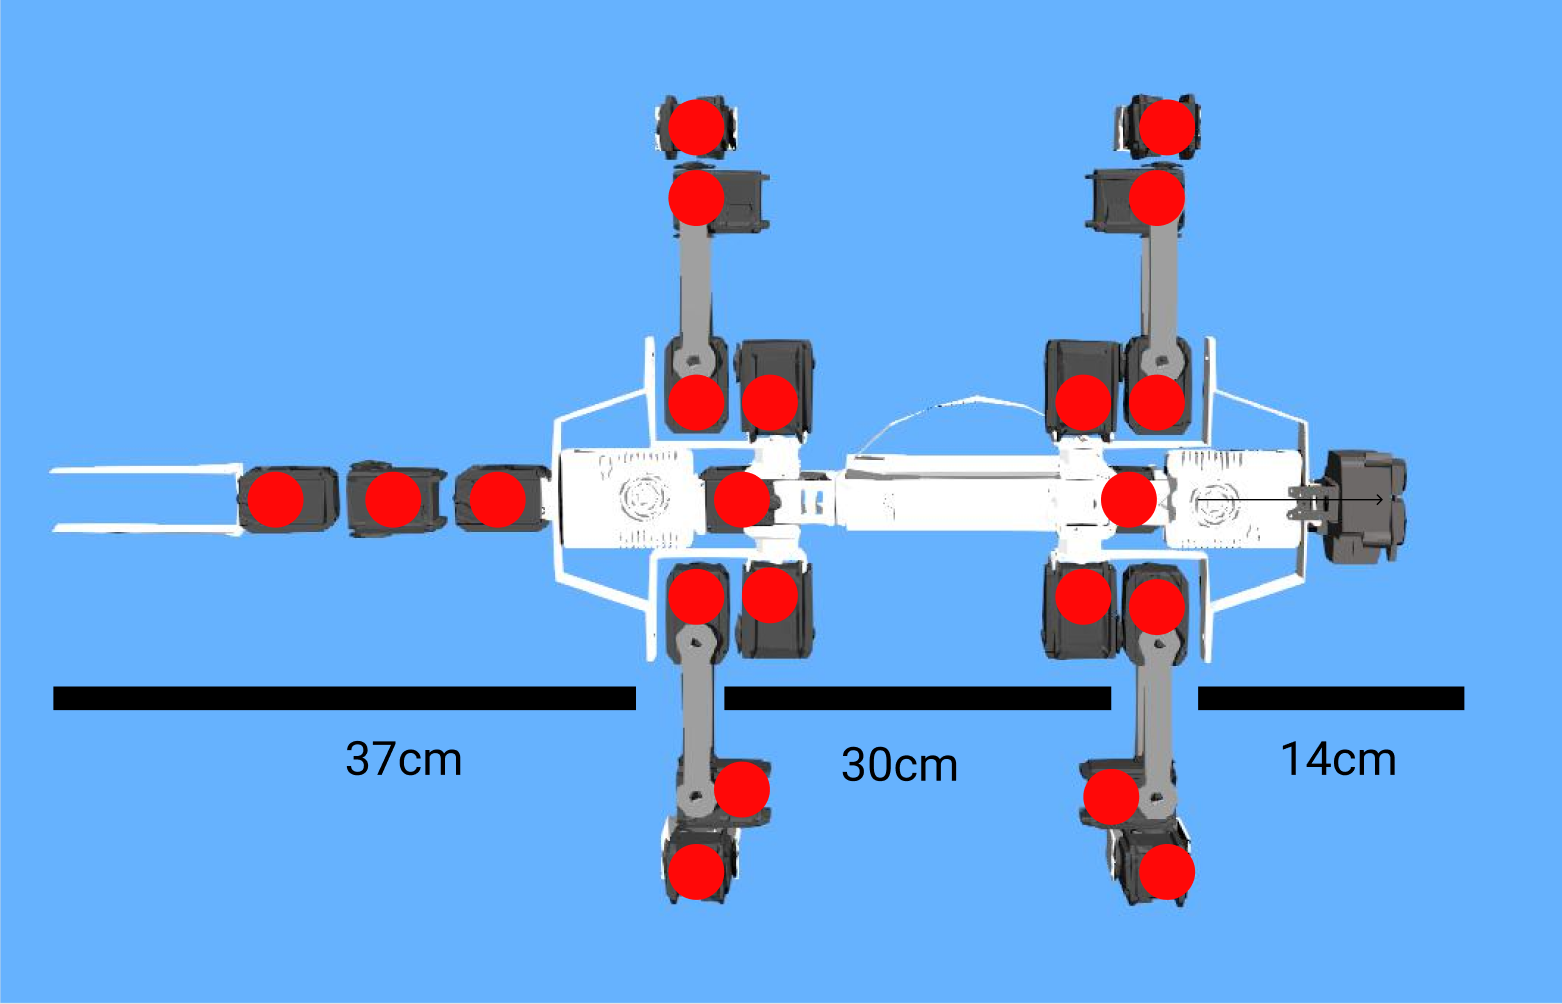
\includegraphics[width=\textwidth]{../img/krock-top-highlight.png}
    \caption{Details highlighted in \emph{Krock}}
       \end{subfigure}
       \caption{}
   	\label{fig:krock-top}

\end{figure}
\emph{Krock}'s moves by lifting and moving forward one leg after the other. The following figure shows the robots going forward.
	\begin{figure}[htbp]
\centering
    	\begin{subfigure}[b]{0.3\textwidth}
			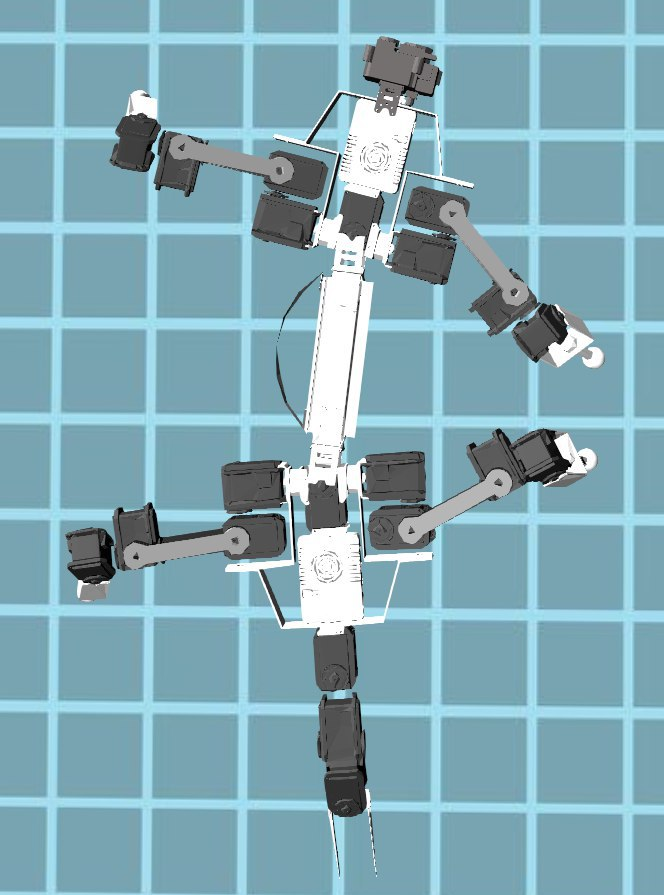
\includegraphics[width=\textwidth]{../img/krock-moving-1}
			\caption{$t=1$}
	    \end{subfigure}
		\begin{subfigure}[b]{0.3\textwidth}
			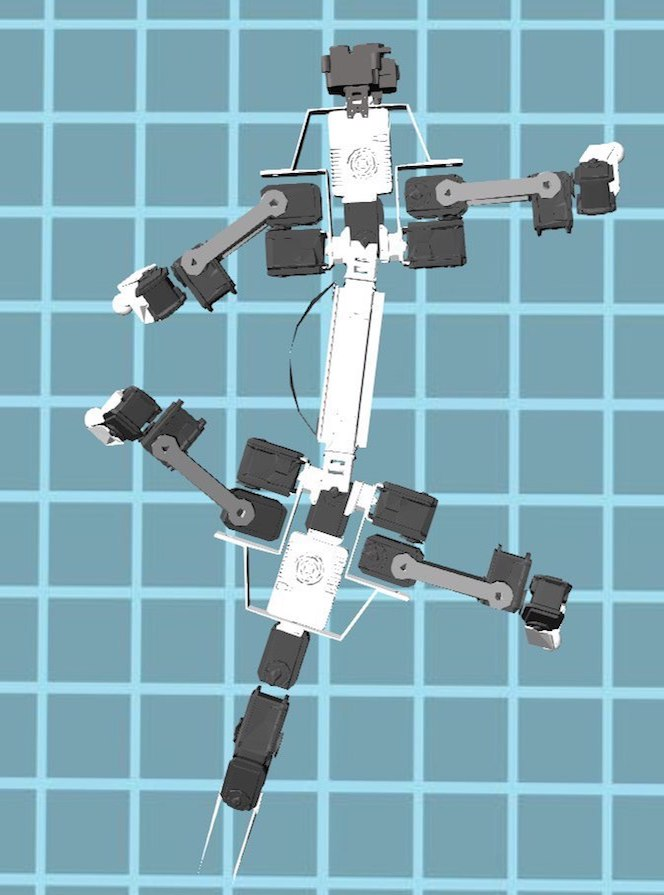
\includegraphics[width=\textwidth]{../img/krock-moving-2}
			\caption{$t=2$}
	    \end{subfigure}	
	   \begin{subfigure}[b]{0.3\textwidth}
			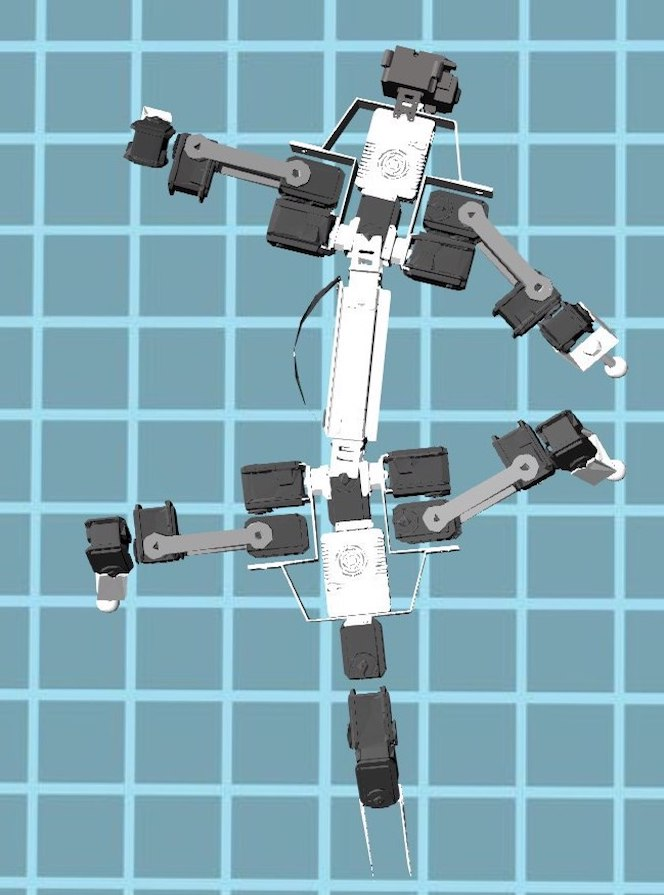
\includegraphics[width=\textwidth]{../img/krock-moving-3}
			\caption{$t=3$}
	    \end{subfigure}	
    \caption{\emph{Krock} moving forward. In this gait configuration, the robot distance from the ground is $16$cm.}
    \label{fig: krock-moving}
	\end{figure}
In our framework we fixed the gait configuration to normal, showed in figure \ref{ig: krock}, where the body is at the same legs' motors height.
% \begin{figure}
% \ref{fig: krock-gait}
% \caption{Krock differents gait configuration.}	
% \end{figure}
\section{Data Gathering}
\label{sec: data-gathering}
This section describe in detail how we created, collected and processed the synthetic dataset used to train the traversability estimator in supervised way.
\subsection{ground generation}
\label{subsec: heightmap-generation}
% To collect the data throught simulation we first need to generate meaningful terrain to be explored by the robot. Each map is stored as a 2D image where each pixel's value represents the terrain's height. For example, the following image shows an heightmap representing a real world quarry and the relative terrain.
% \begin{figure}[htbp]
%     \centering
%         \begin{subfigure}[b]{0.45\textwidth}
%             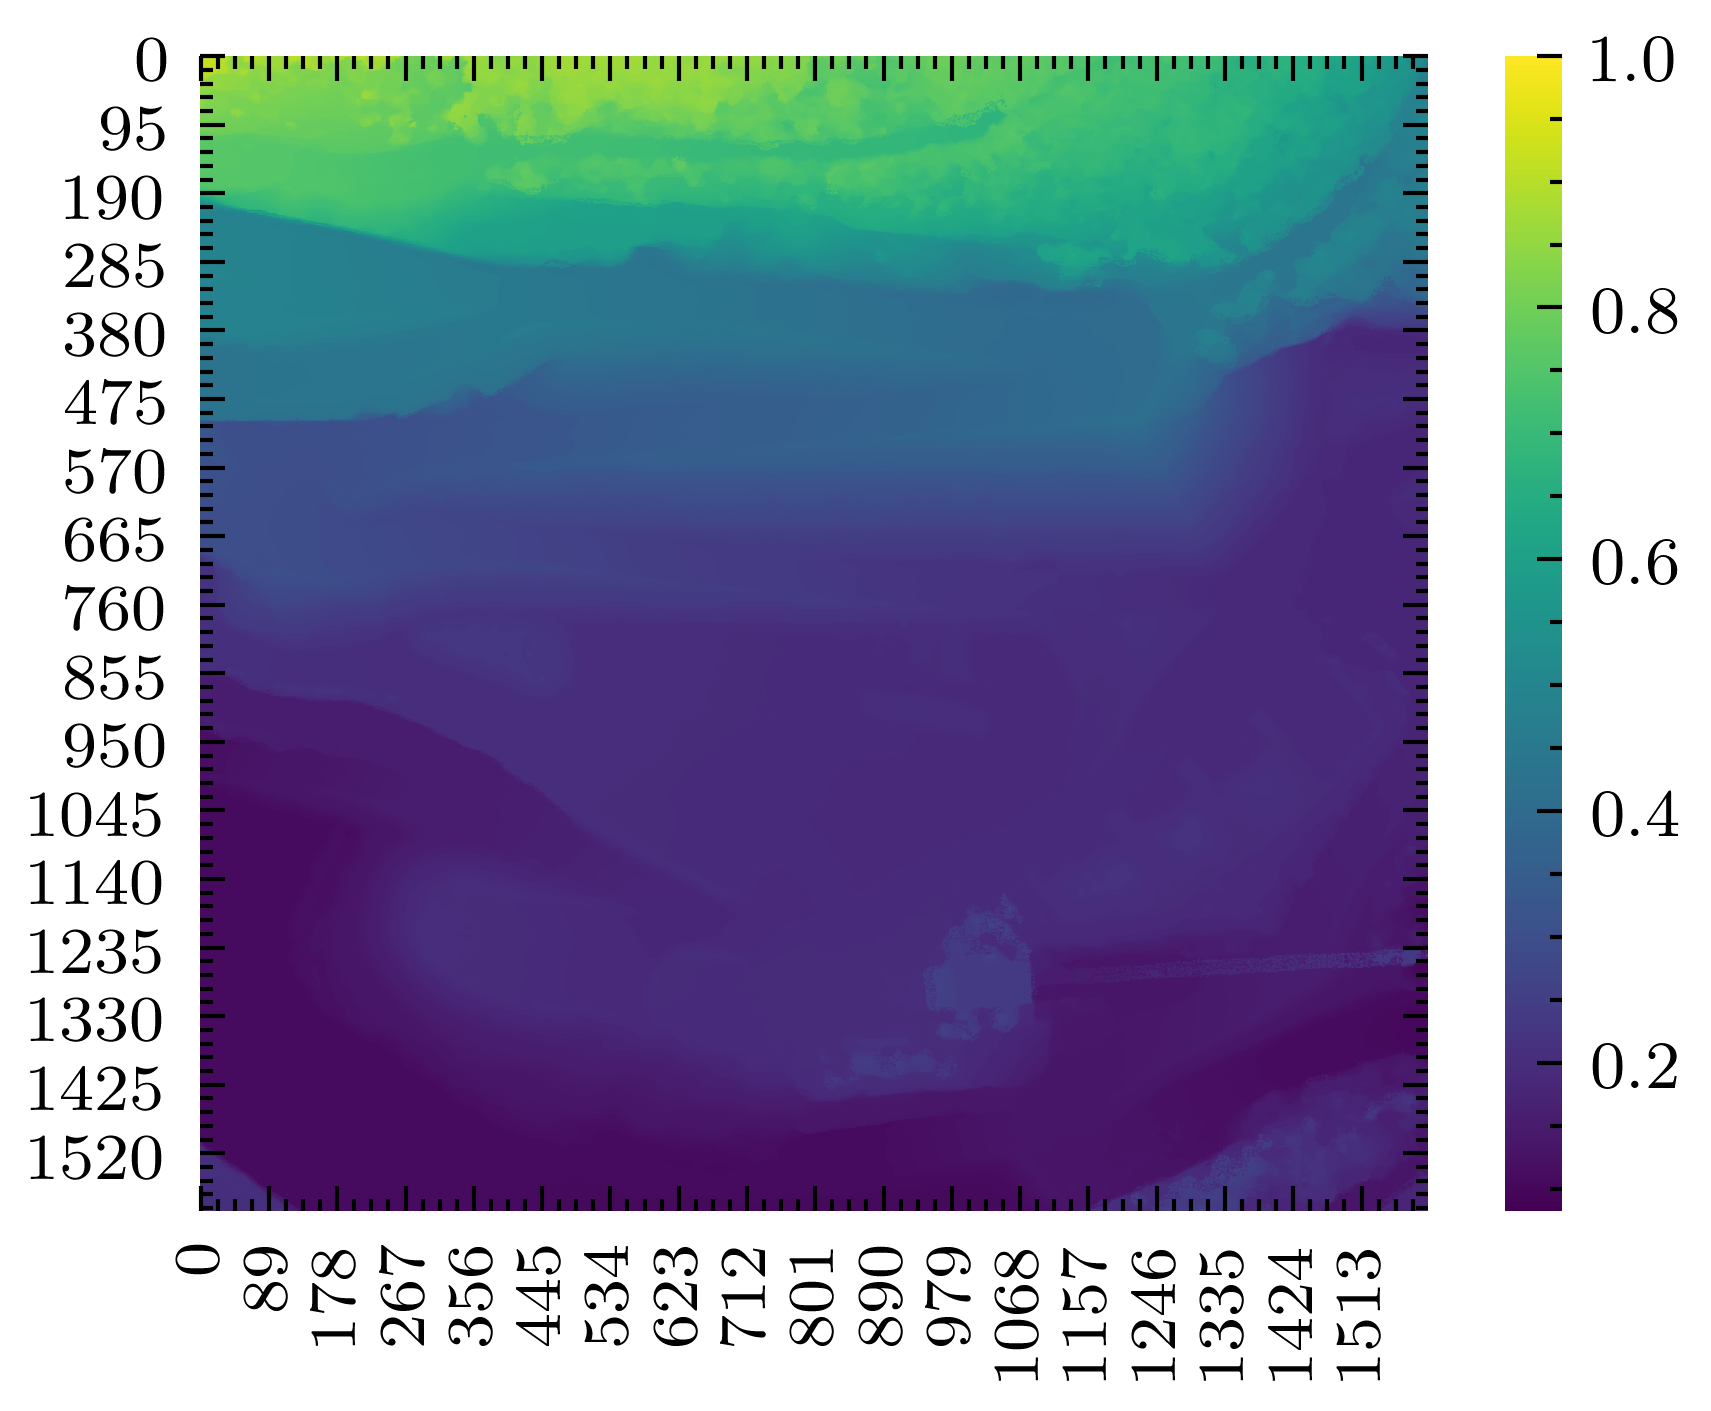
\includegraphics[width=\textwidth]{../img/hm/querry-big-10.png}
%             \caption{Heightmap.}
%         \end{subfigure}
%         \begin{subfigure}[b]{0.45\linewidth}
%             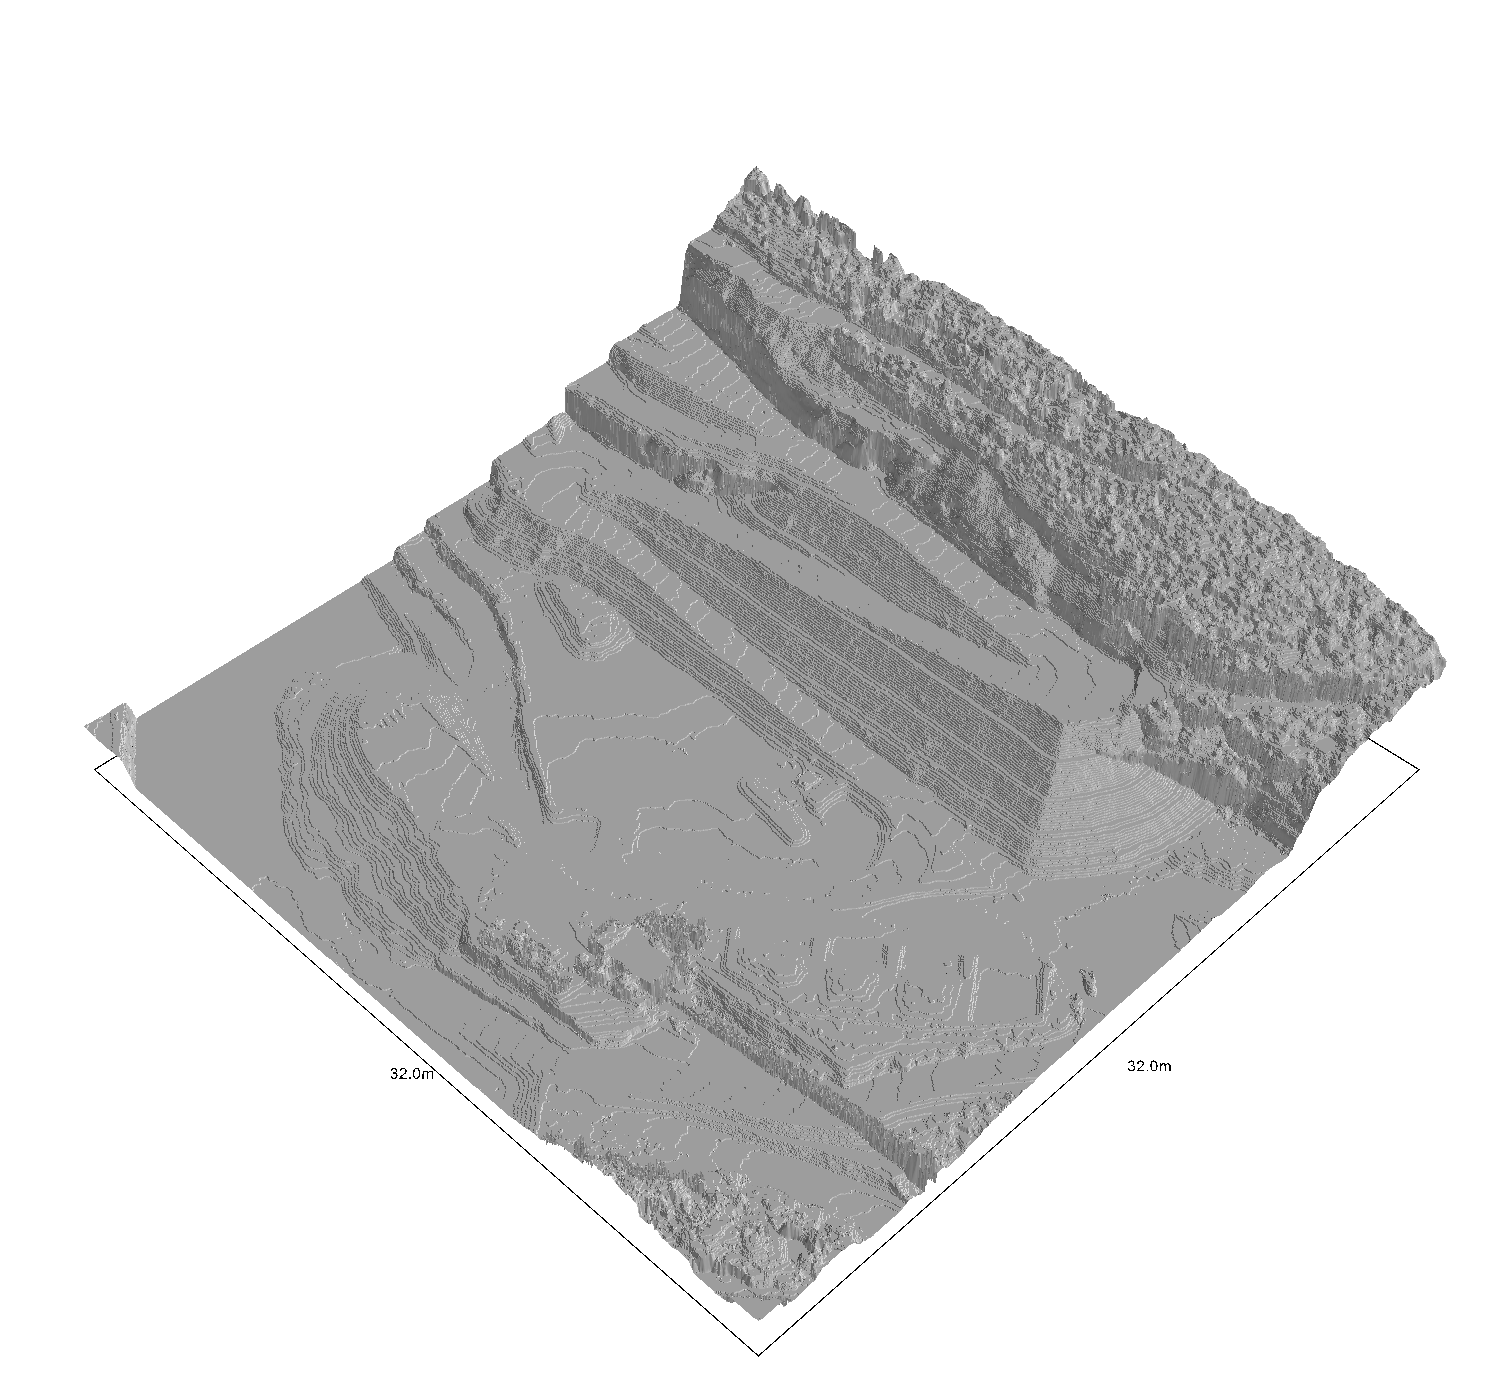
\includegraphics[width=\textwidth]{../img/hm3d_borders/querry-big-10.png}
%             \caption{3D rendered}
%             \end{subfigure}    
%     \caption{This image shows an heightmap and the 3D render of a quarry.}
%     \end{figure}rom each trajectory, what you did in simulation was to command the robot to move forward for 2 secs, i.e. created a trajectory from the spawning pose to the pose reached at the end of those 2 secs of moving forward. Ergo, you have to extract the patches at each pose of the trajectory generated at simulation time
We created thirty rom each trajectory, what you did in simulation was to command the robot to move forward for 2 secs, i.e. created a trajectory from the spawning pose to the pose reached at the end of those 2 secs of moving forward. Ergo, you have to extract the patches at each pose of the trajectory generated at simulation timelution of $0.02cm/pixel$ using 2D simplex noise variant of Perlin noise \cite{perlin}, a widely used technirom each trajectory, what you did in simulation was to command the robot to move forward for 2 secs, i.e. created a trajectory from the spawning pose to the pose reached at the end of those 2 secs of moving forward. Ergo, you have to extract the patches at each pose of the trajectory generated at simulation timelitterature. We divide the maps into five main categories of terrains to cluster differents ground features: $rom each trajectory, what you did in simulation was to command the robot to move forward for 2 secs, i.e. created a trajectory from the spawning pose to the pose reached at the end of those 2 secs of moving forward. Ergo, you have to extract the patches at each pose of the trajectory generated at simulation timepes$/$ramps$ and $holes$.
\paragraph{Bumps:} 
We genered four different maps with increasing bumps' height using simplex noise. 
\begin{figure}[H]
    \centering
        \begin{subfigure}[b]{0.23\textwidth}
            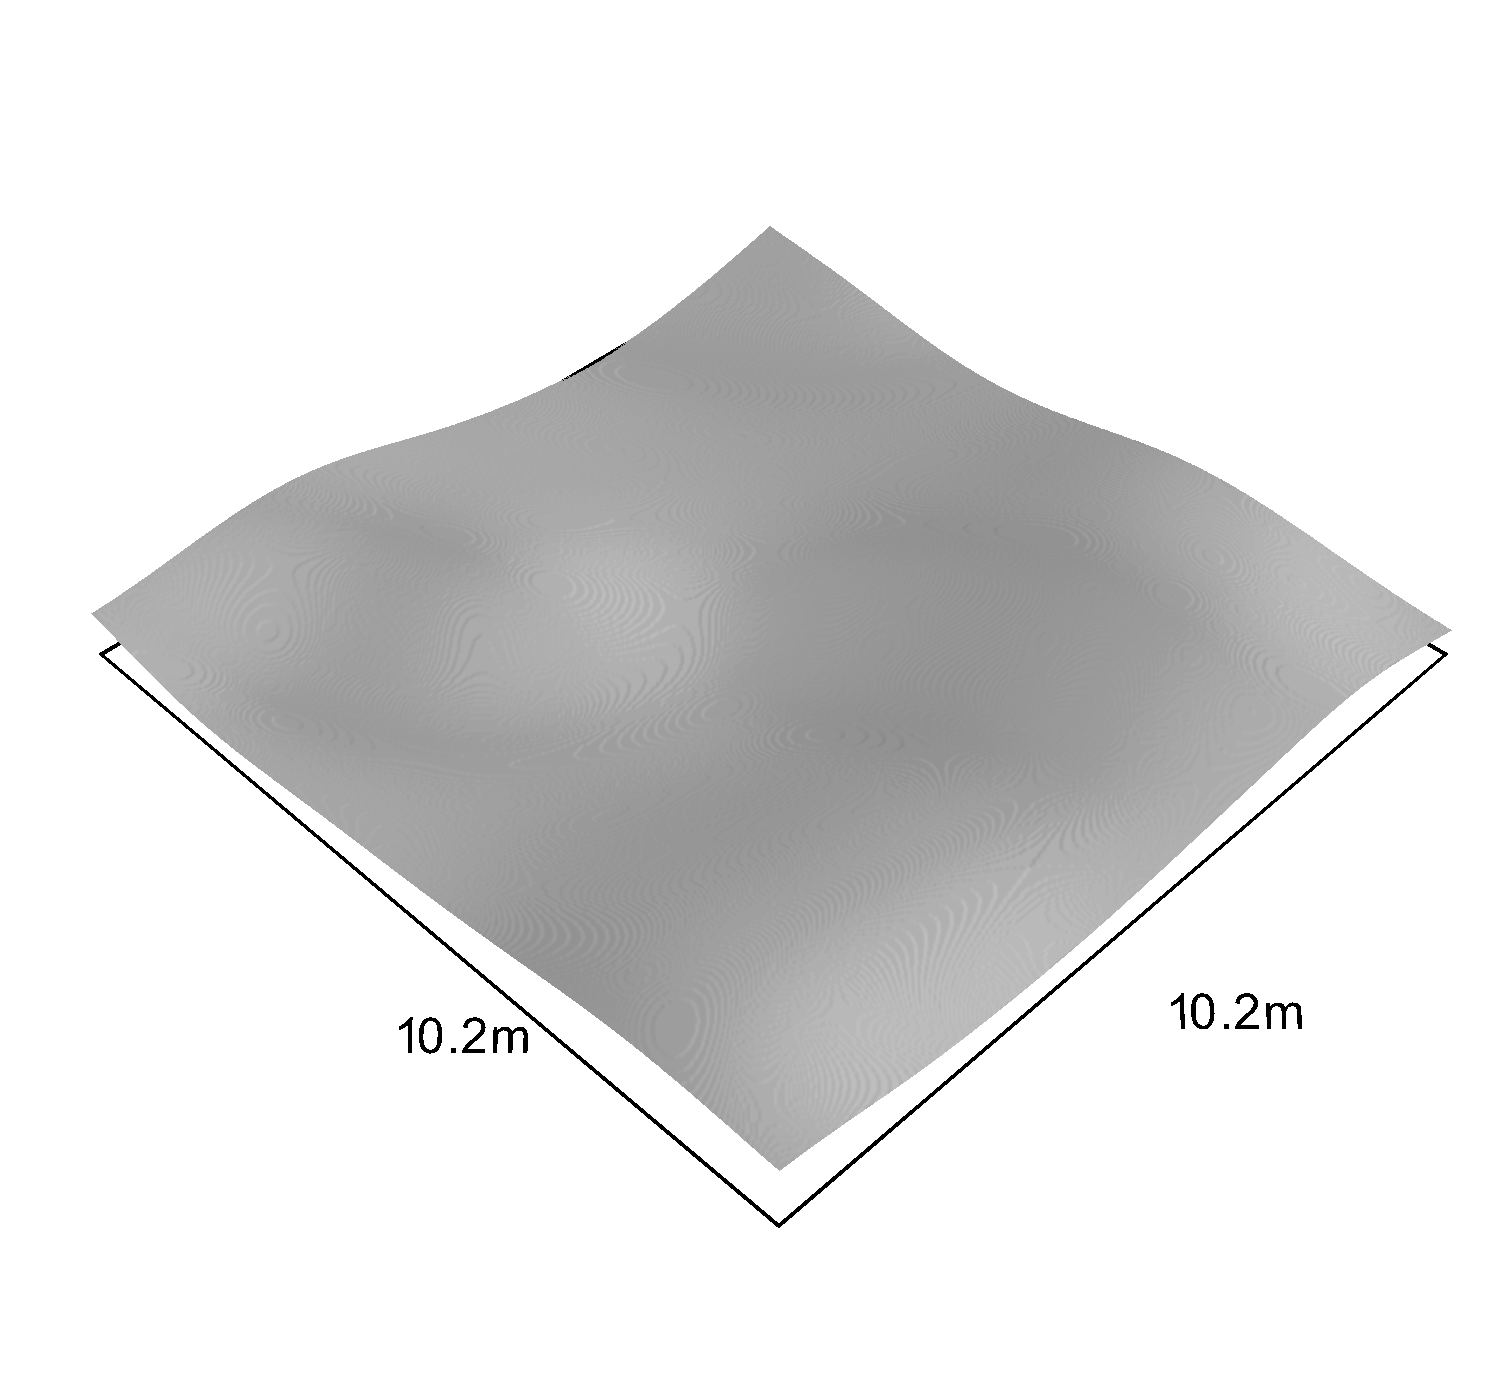
\includegraphics[width=\textwidth]{../img/hm3d_borders/bumps0.png}
            \caption{\emph{bumps0}}
        \end{subfigure}
        \begin{subfigure}[b]{0.23\linewidth}
            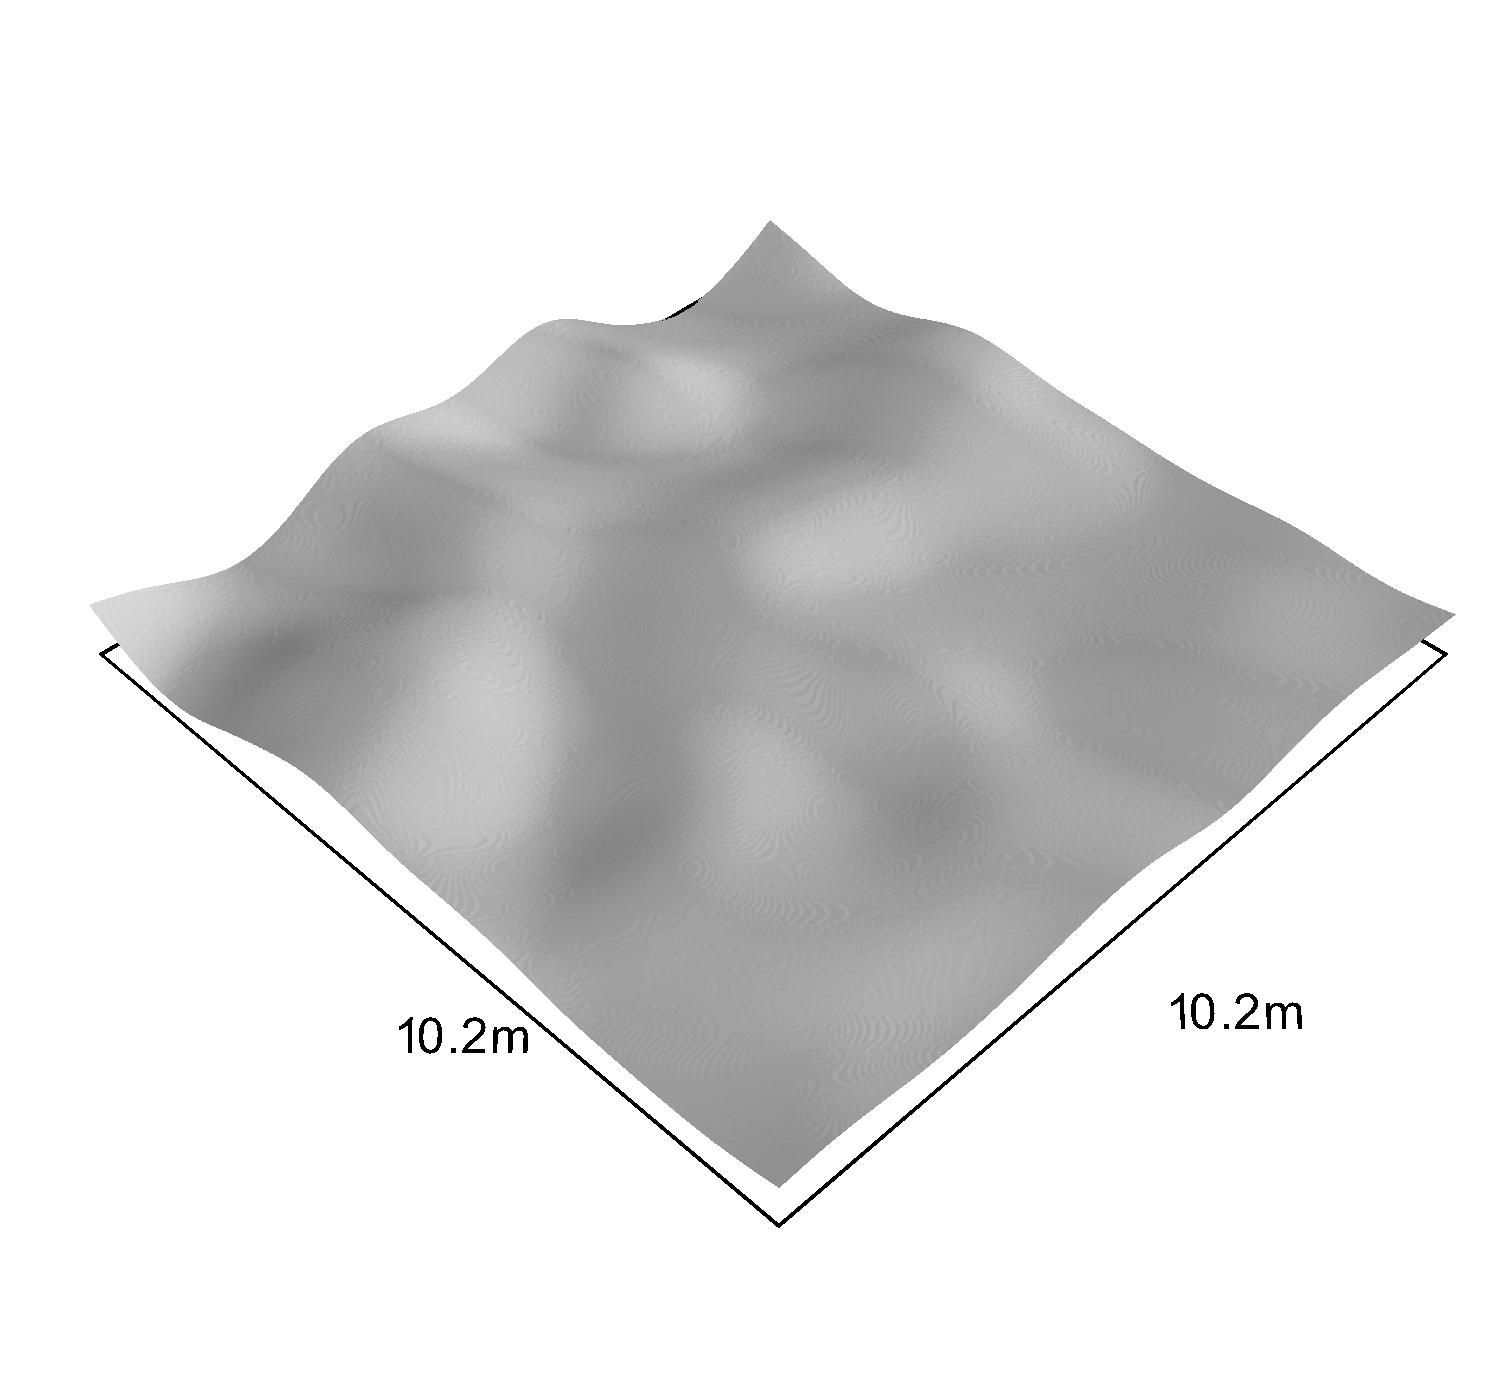
\includegraphics[width=\textwidth]{../img/hm3d_borders/bumps1.png}
            \caption{\emph{bumps1}}
            \end{subfigure}    
          \begin{subfigure}[b]{0.23\textwidth}
            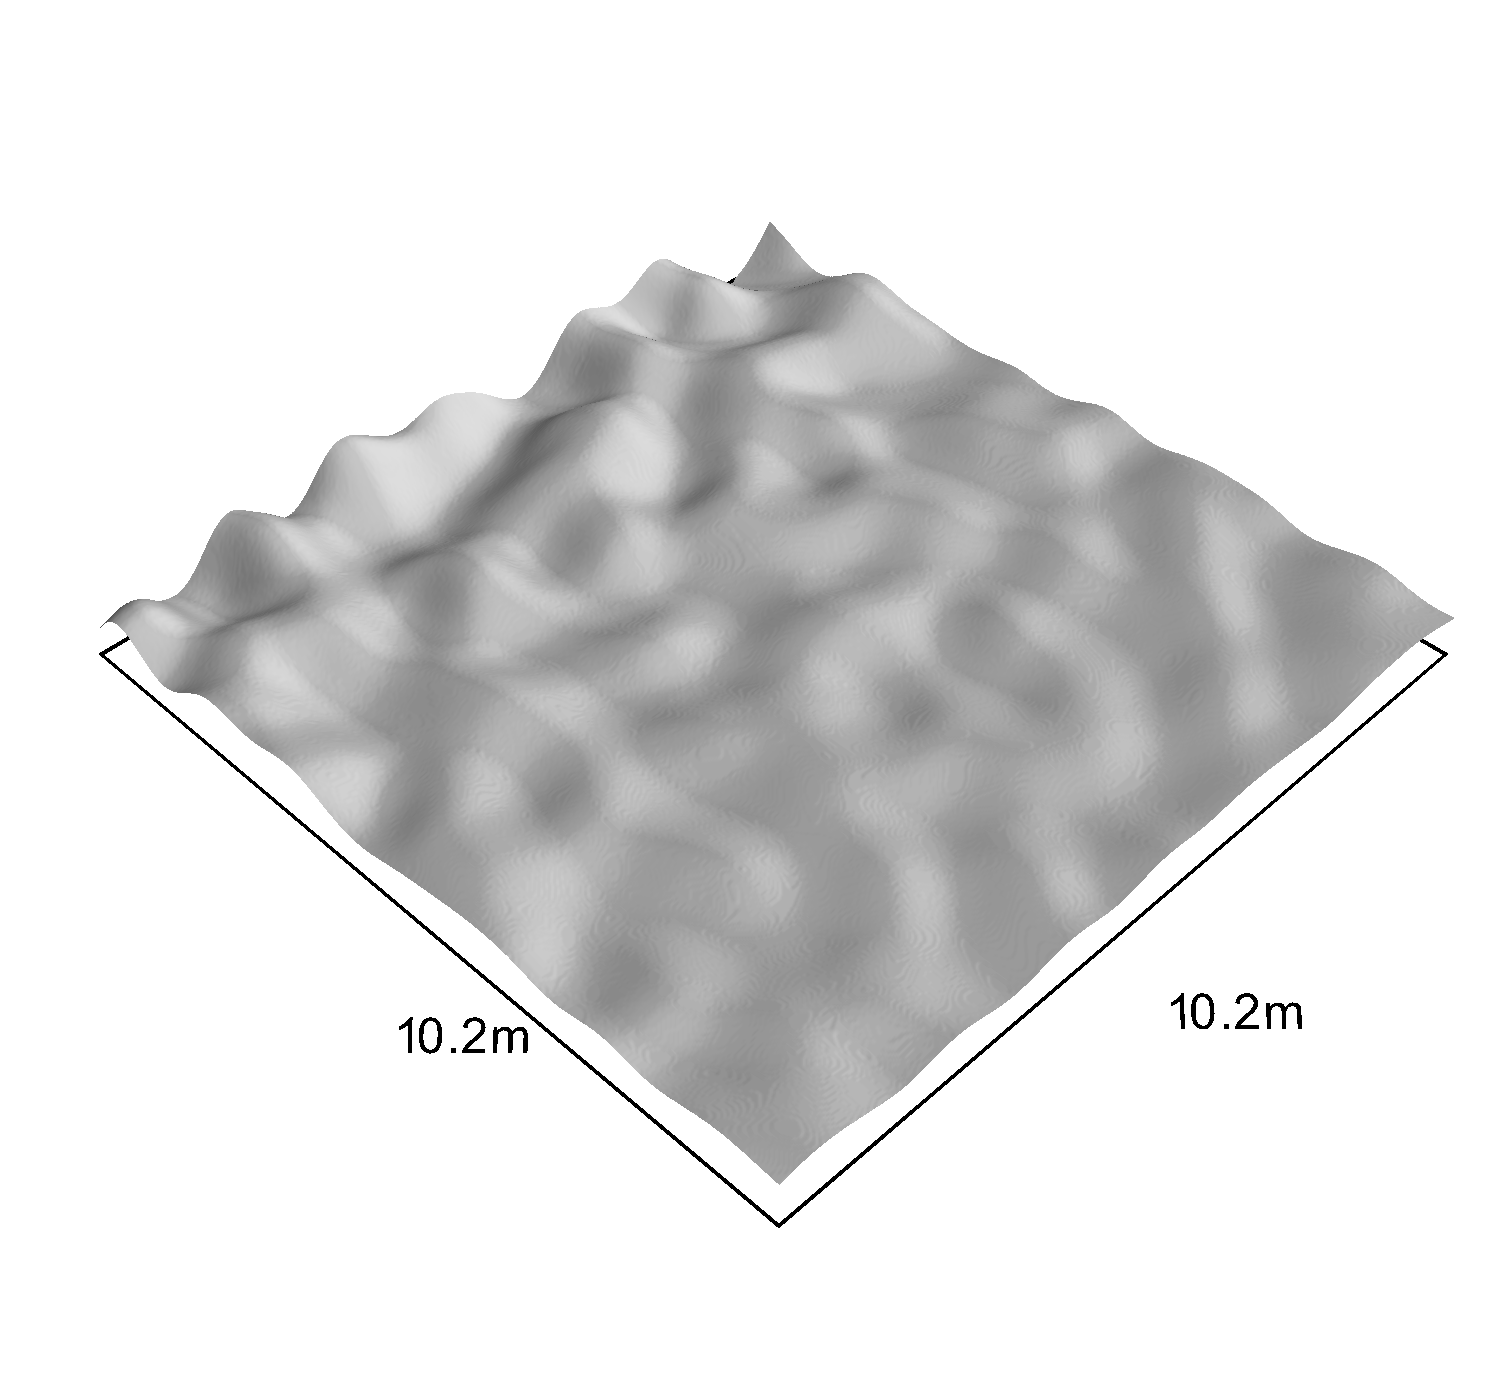
\includegraphics[width=\textwidth]{../img/hm3d_borders/bumps2.png}
            \caption{\emph{bumps2}}
        \end{subfigure}    
        \begin{subfigure}[b]{0.23\textwidth}
            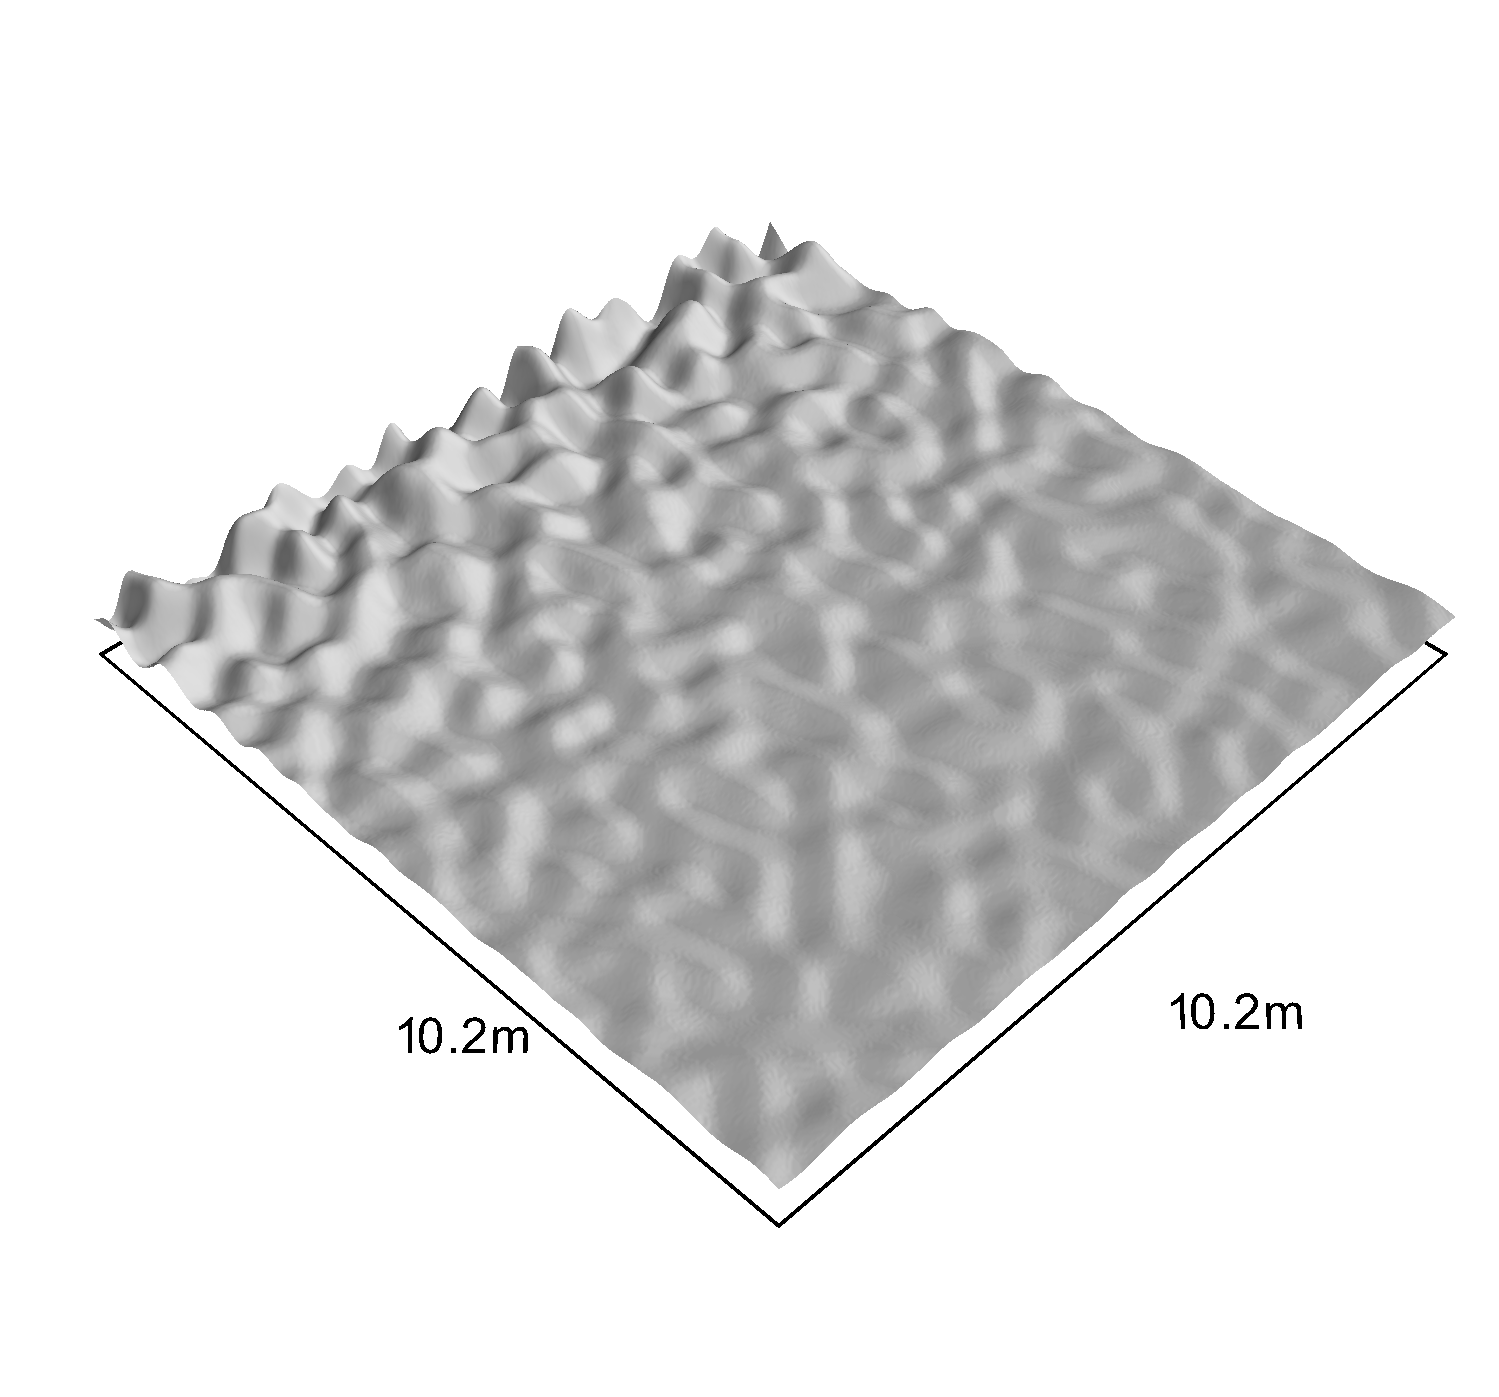
\includegraphics[width=\textwidth]{../img/hm3d_borders/bumps3.png}
            \caption{\emph{bumps3}}
        \end{subfigure}    
    \caption{Bumps maps.}
\end{figure}
\paragraph{Bars:} In these maps there are wall with different shapes and heights. 
\begin{figure}[H]
    \centering
        \begin{subfigure}[b]{0.23\textwidth}
            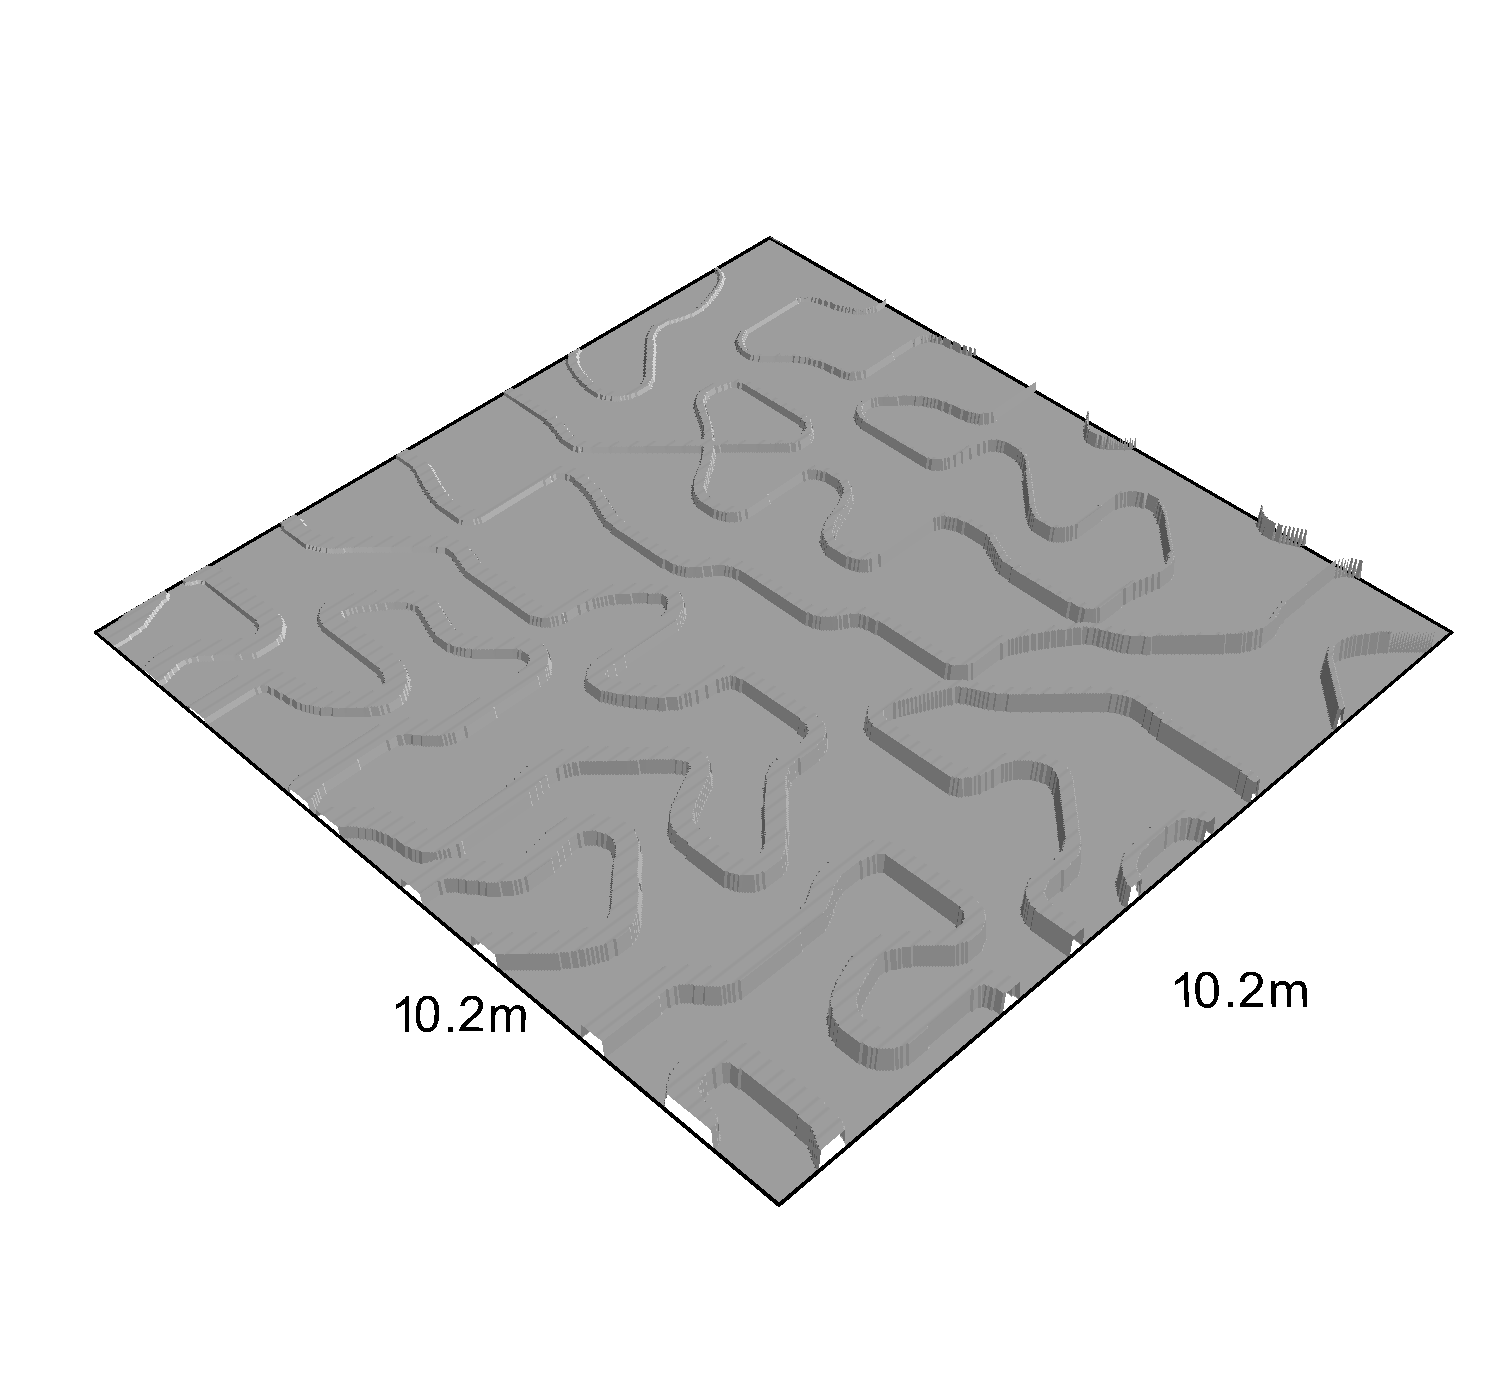
\includegraphics[width=\textwidth]{../img/hm3d_borders/bars1.png}
            \caption{\emph{bars1}}
        \end{subfigure}
        \begin{subfigure}[b]{0.23 \linewidth}
            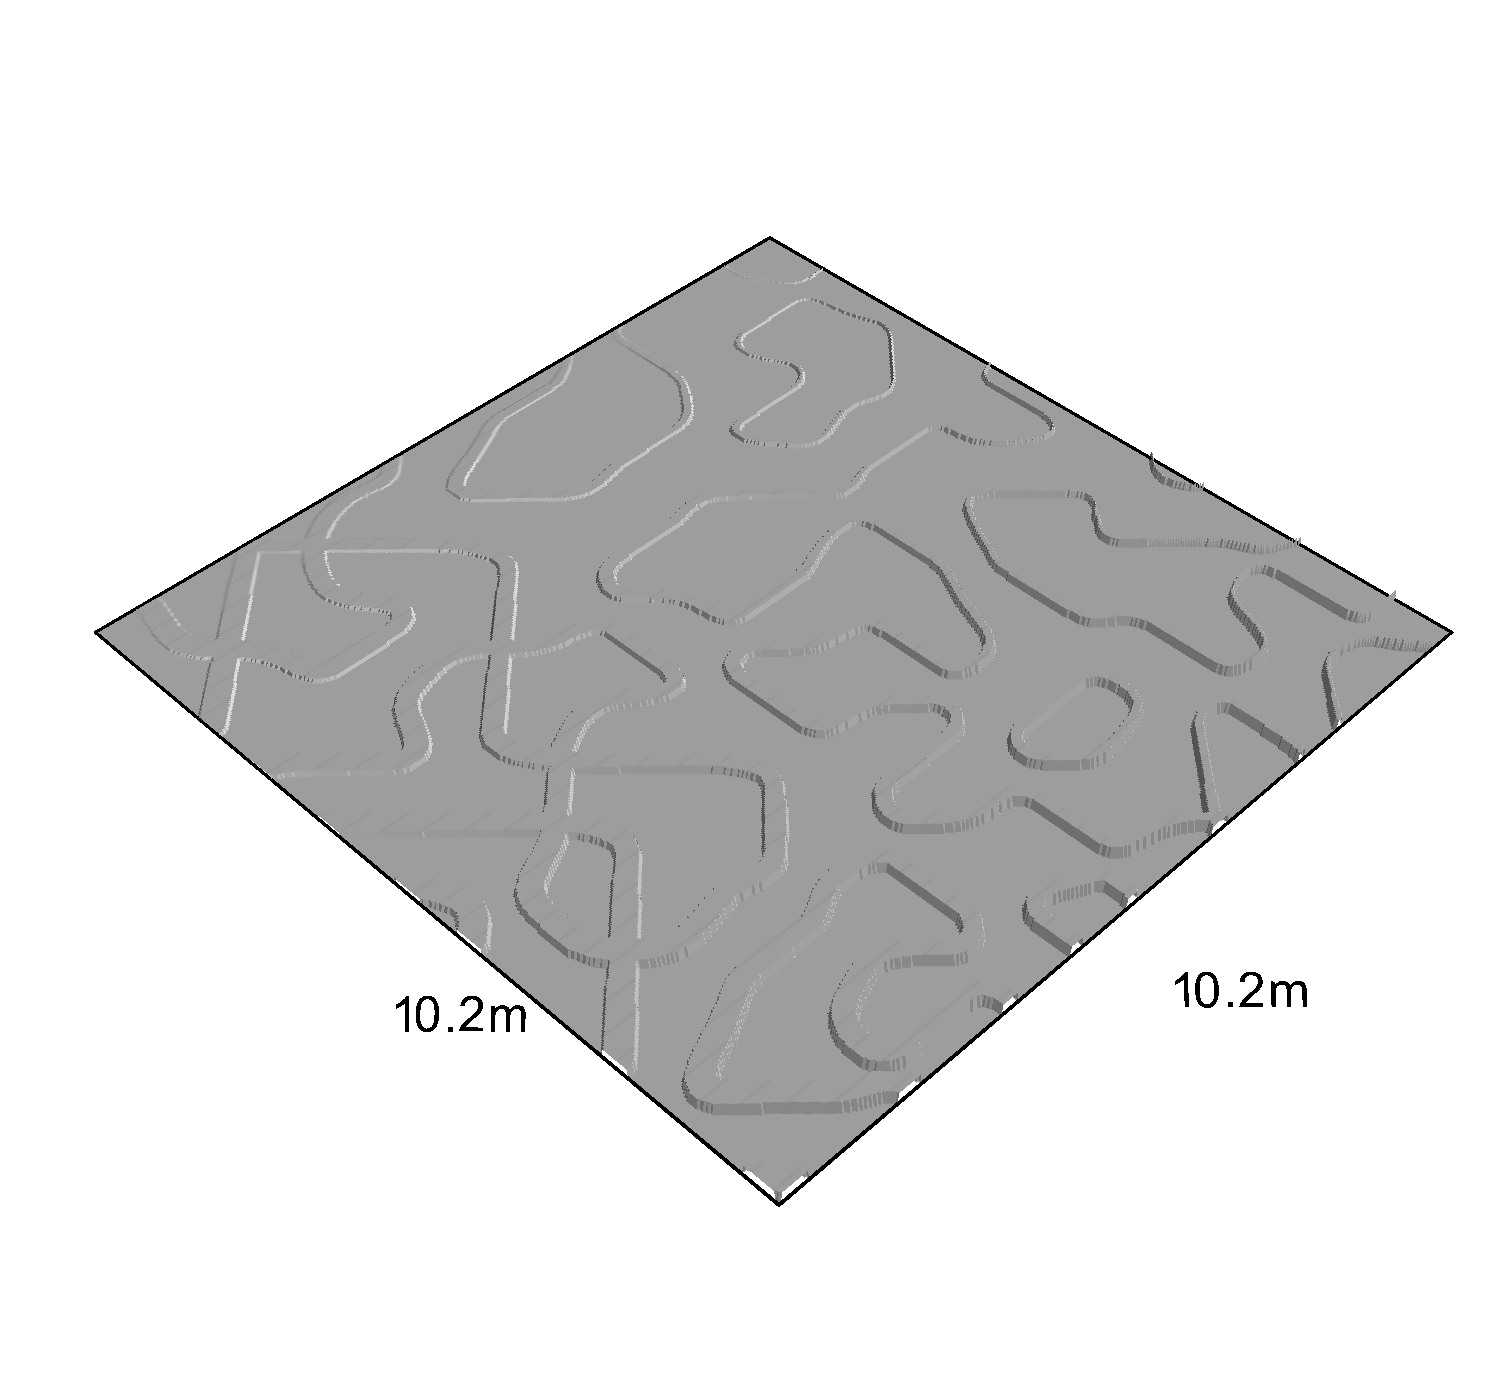
\includegraphics[width=\textwidth]{../img/hm3d_borders/bars3.png}
            \caption{\emph{bars3}}
            \end{subfigure}     
    \caption{Bars maps.}
    \label{fig : bars-maps}
\end{figure}
\paragraph{Rails:} Flat grounds with slots.
\begin{figure}[H]
    \centering
        \begin{subfigure}[b]{0.23\textwidth}
            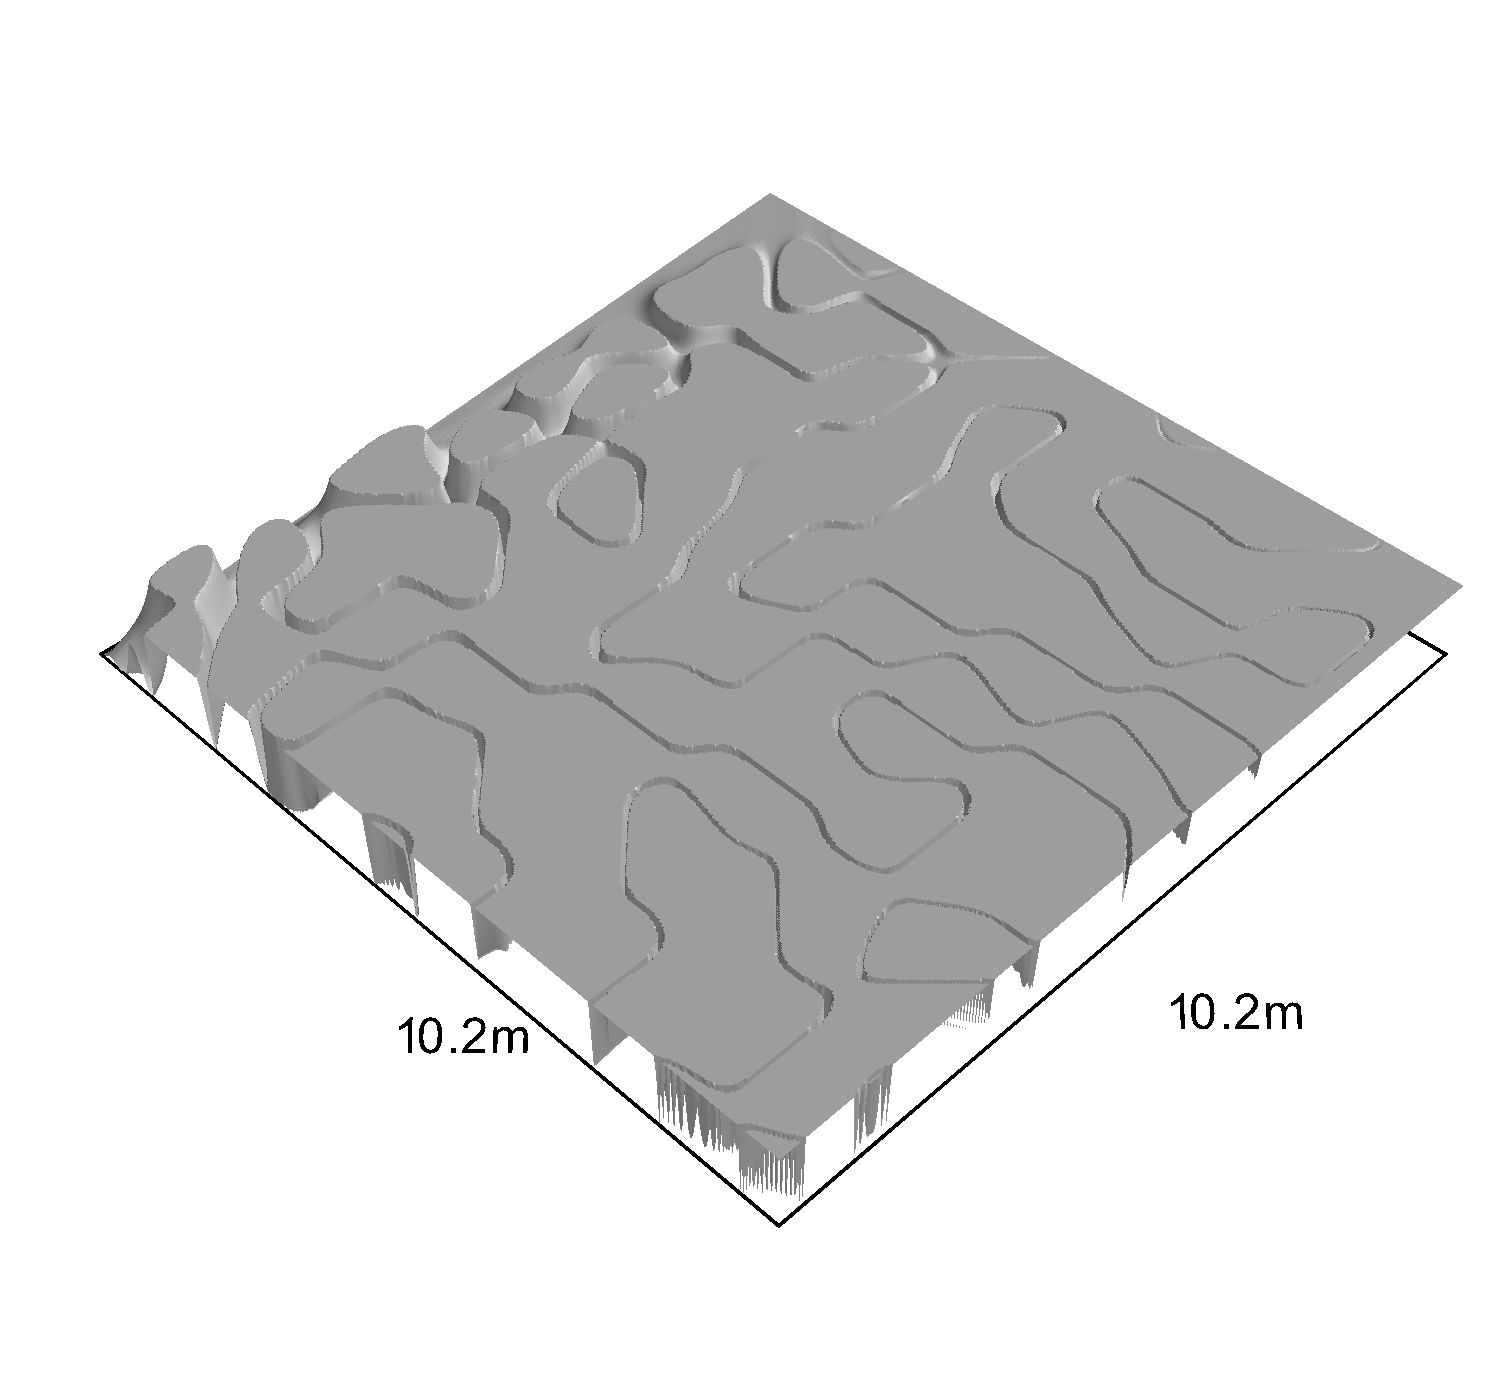
\includegraphics[width=\textwidth]{../img/hm3d_borders/rails1.png}
            \caption{\emph{rails1}}
        \end{subfigure}
        \begin{subfigure}[b]{0.23\linewidth}
            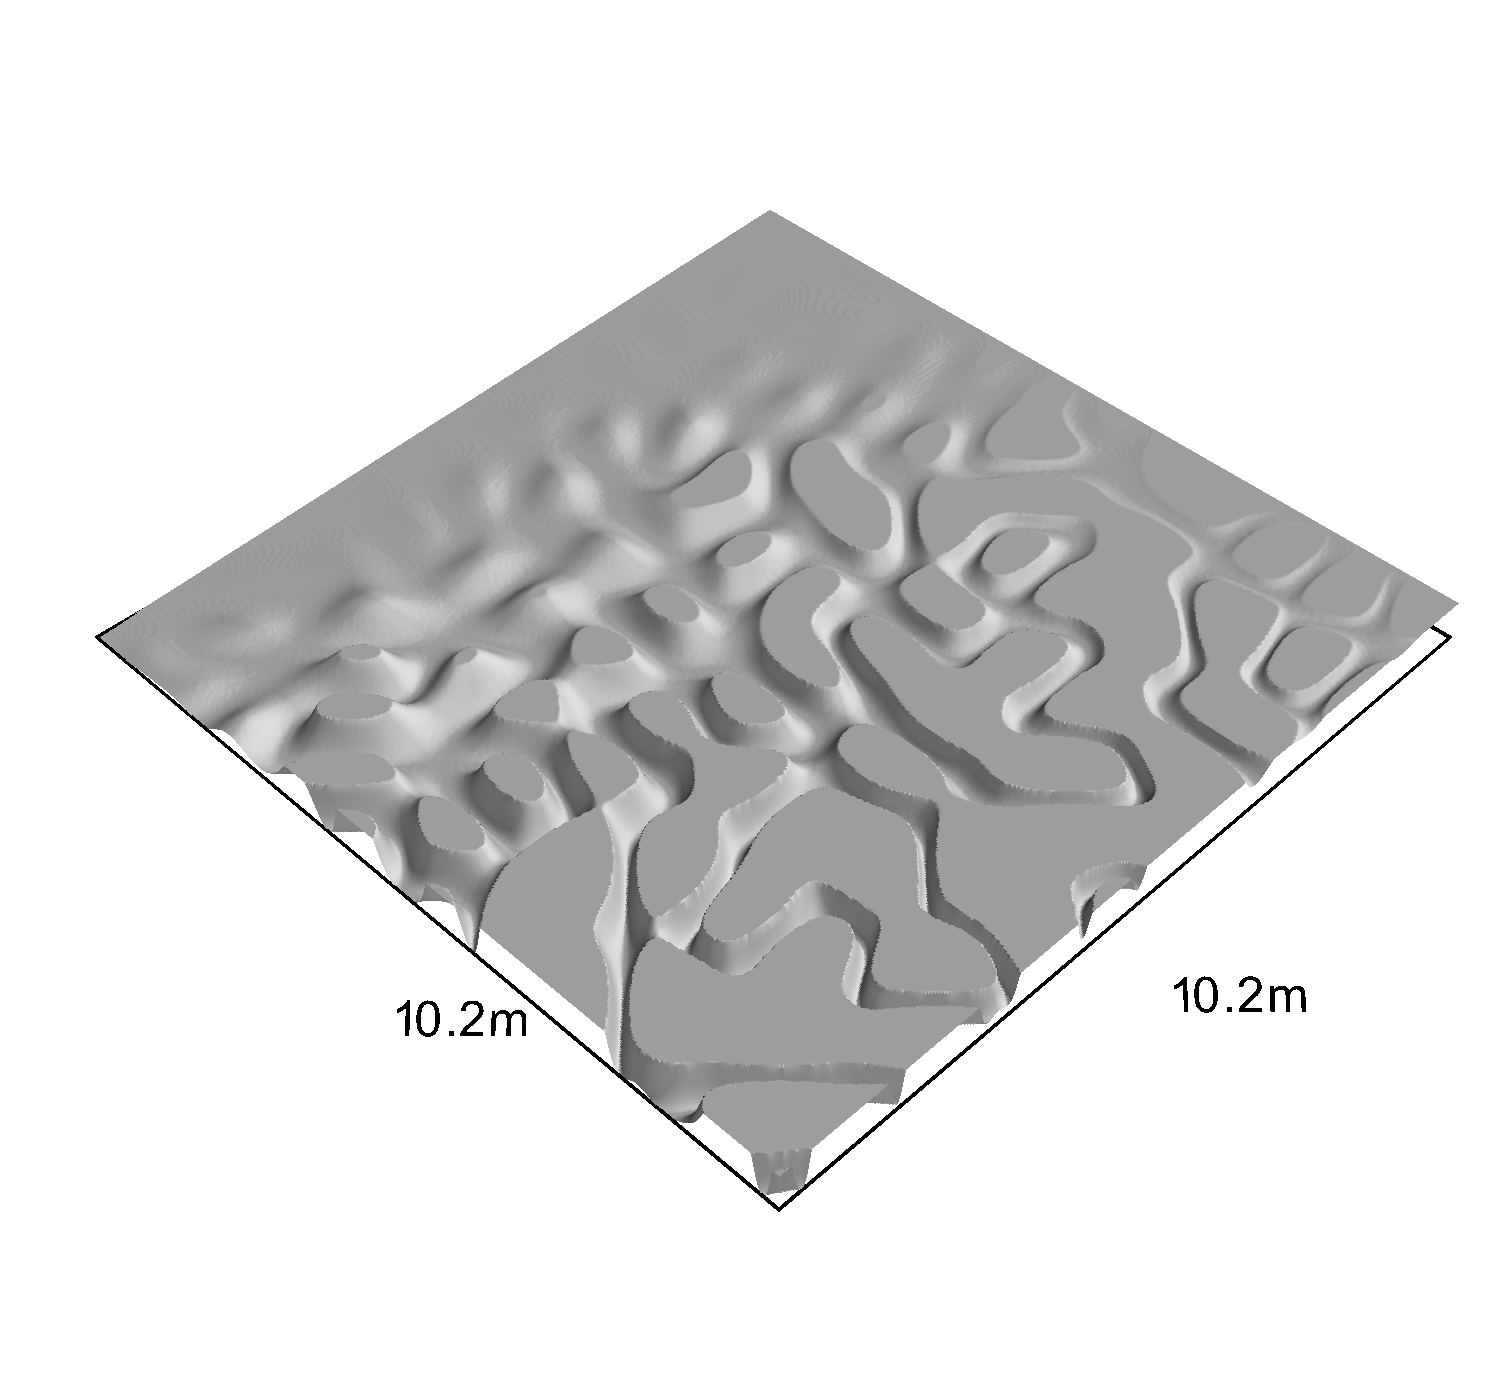
\includegraphics[width=\textwidth]{../img/hm3d_borders/rails2.png}
            \caption{\emph{rails2}}
            \end{subfigure}    
          \begin{subfigure}[b]{0.23\textwidth}
            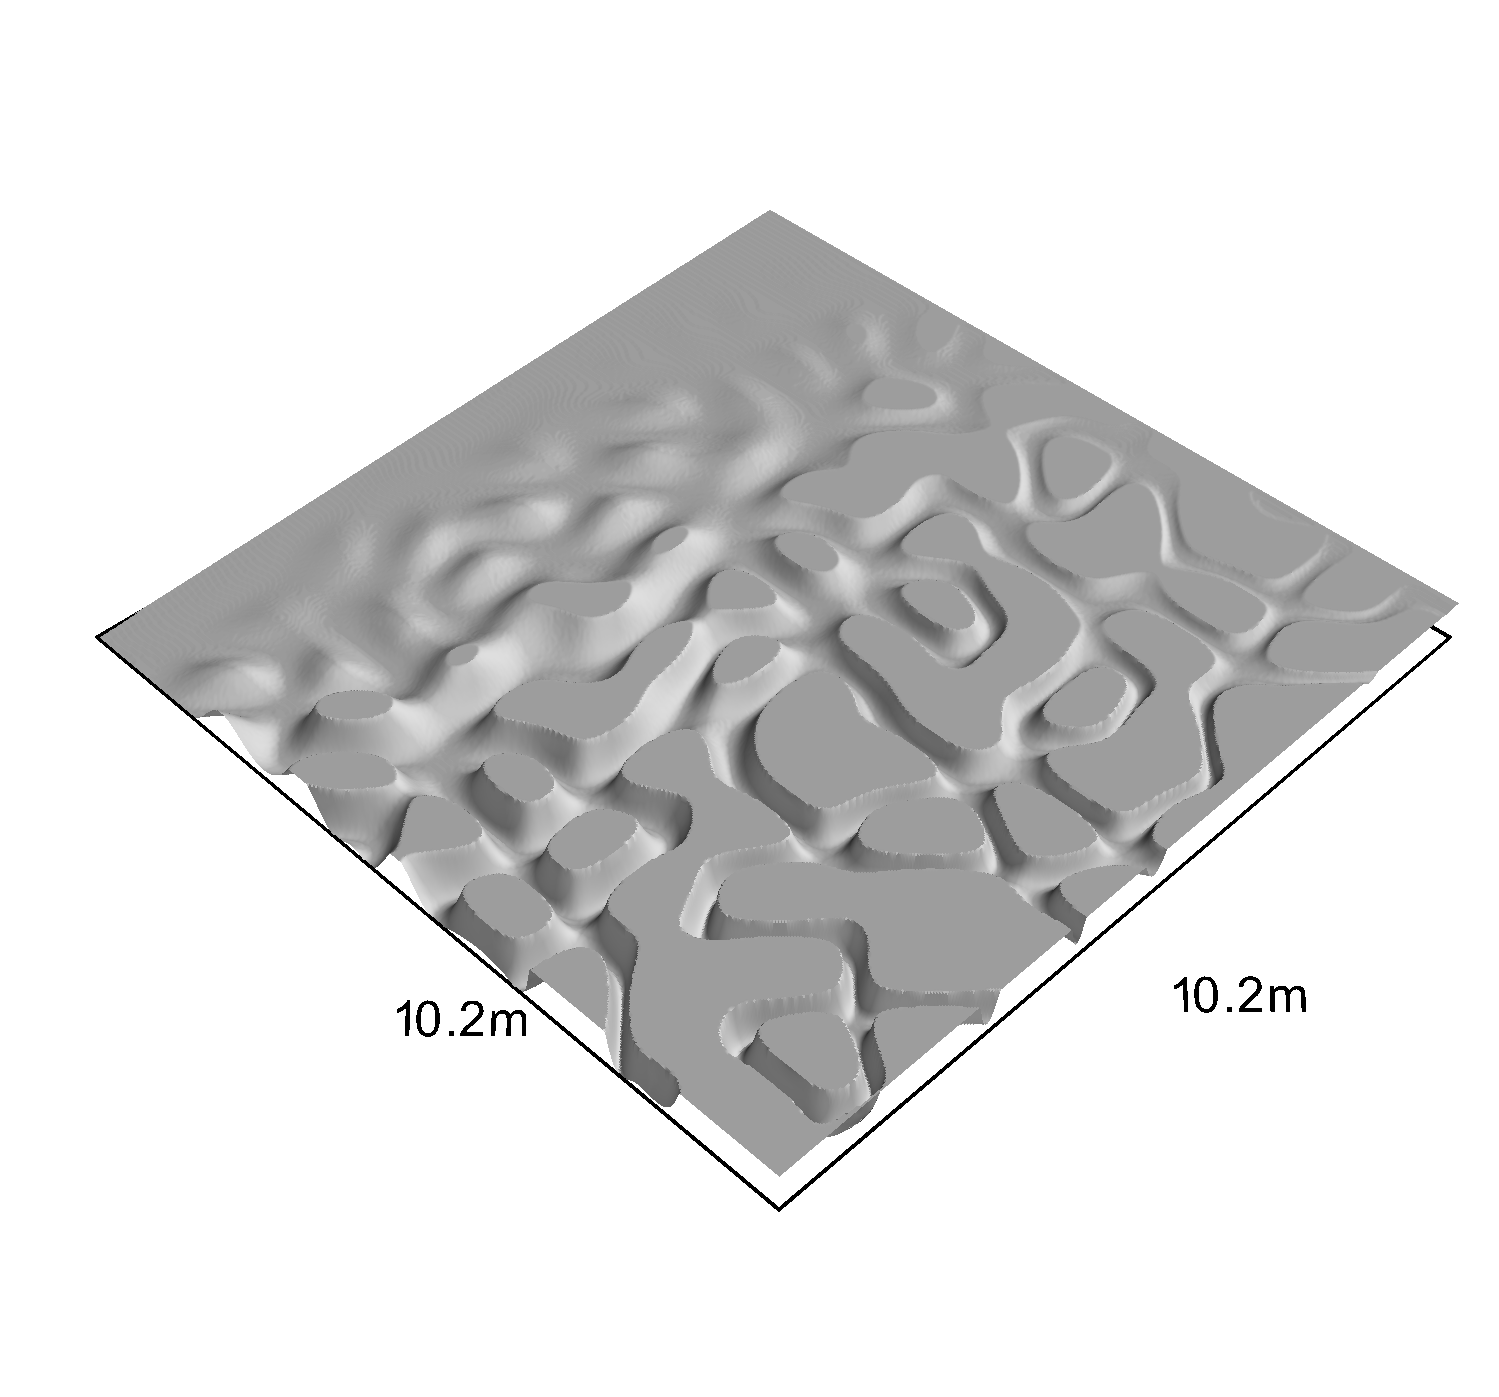
\includegraphics[width=\textwidth]{../img/hm3d_borders/rails3.png}
            \caption{\emph{rails3}}
        \end{subfigure}    
    \caption{Rails maps.}
\end{figure}
\paragraph{Steps:} These are maps with various steps at increasing distance and frequency.
\begin{figure}[H]
    \centering
        \begin{subfigure}[b]{0.23\textwidth}
            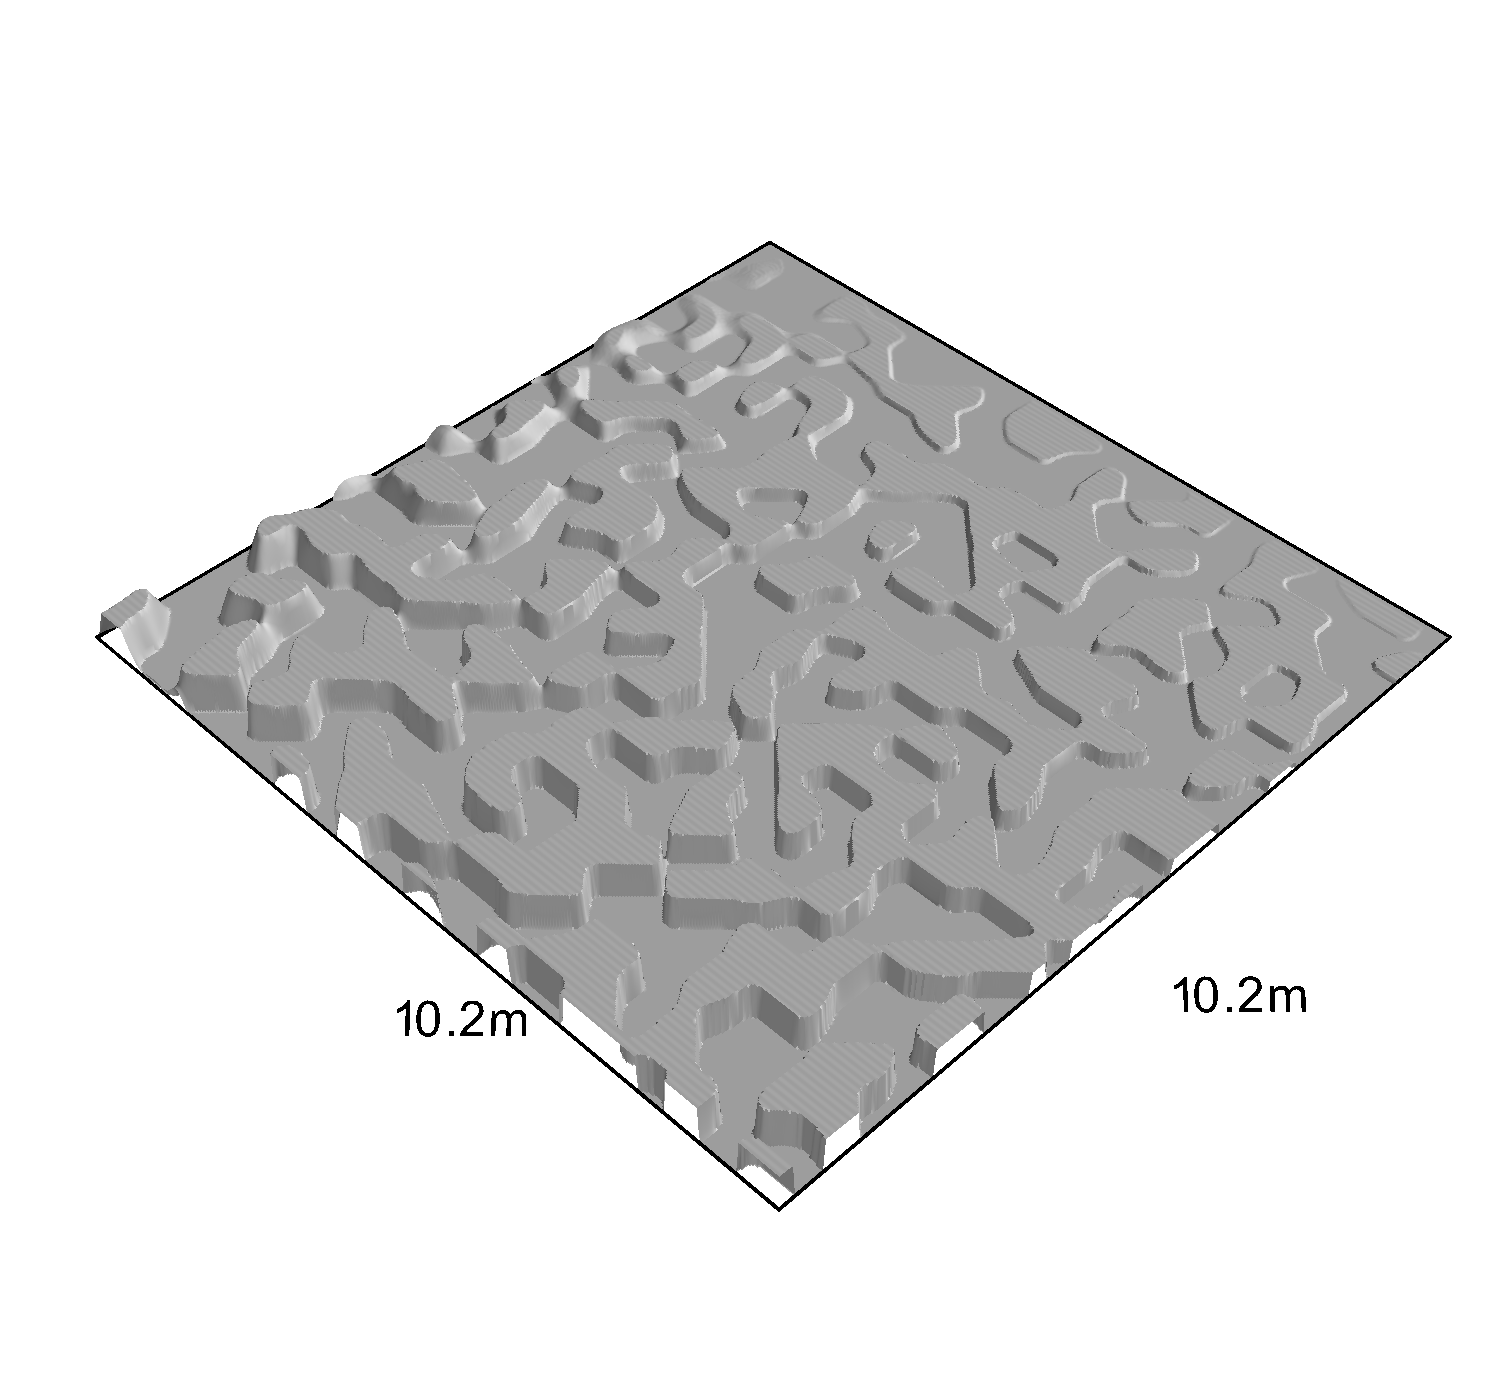
\includegraphics[width=\textwidth]{../img/hm3d_borders/steps1.png}
            \caption{\emph{steps1}}
        \end{subfigure}
        \begin{subfigure}[b]{0.23\linewidth}
            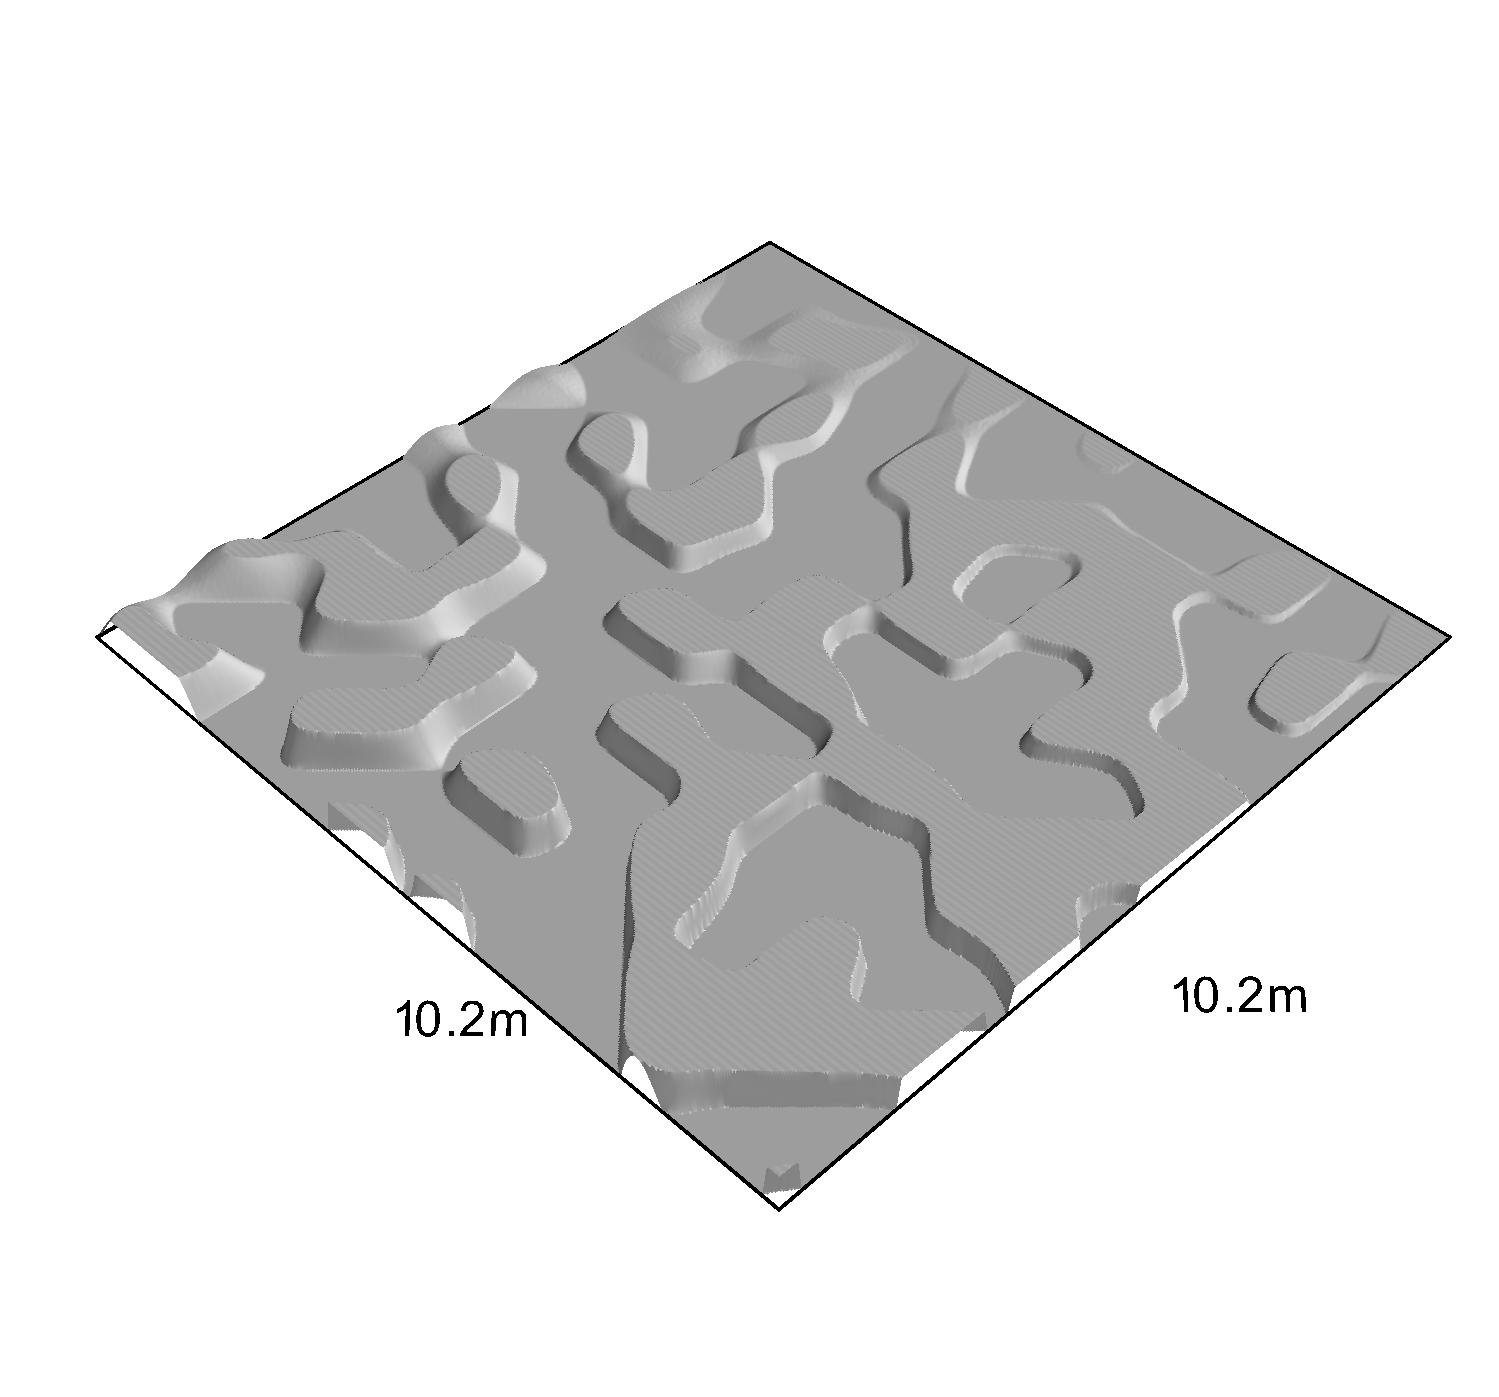
\includegraphics[width=\textwidth]{../img/hm3d_borders/steps2.png}
            \caption{\emph{steps2}}
            \end{subfigure}    
          \begin{subfigure}[b]{0.23\textwidth}
            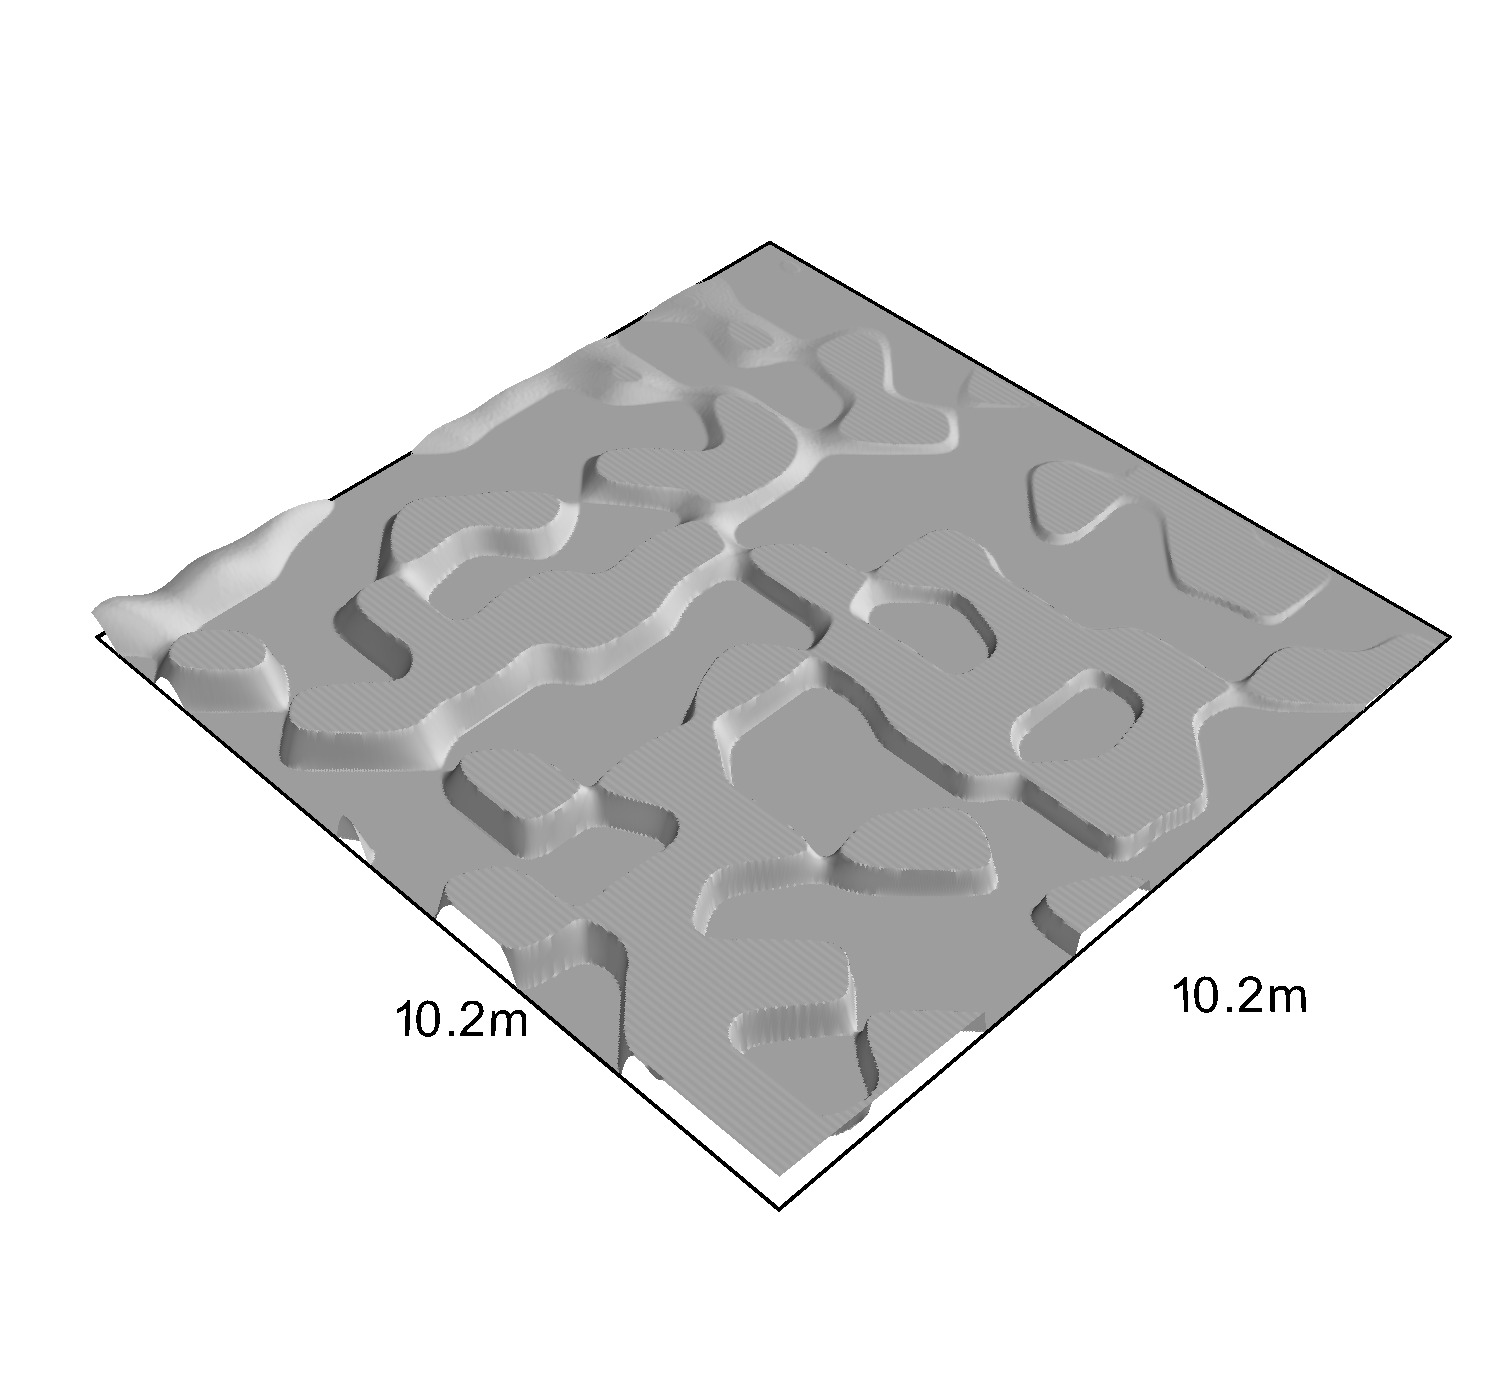
\includegraphics[width=\textwidth]{../img/hm3d_borders/steps3.png}
            \caption{\emph{steps3}}
        \end{subfigure}    
    \caption{Steps maps.}
\end{figure}

\paragraph{Slopes/Ramps:} Maps composed by uneven terrain scaled by different height factors from $3$ to $5$ used to include samples where \emph{Krock} has to climb.
\begin{figure}[H]
    \centering
        \begin{subfigure}[b]{0.23\textwidth}
            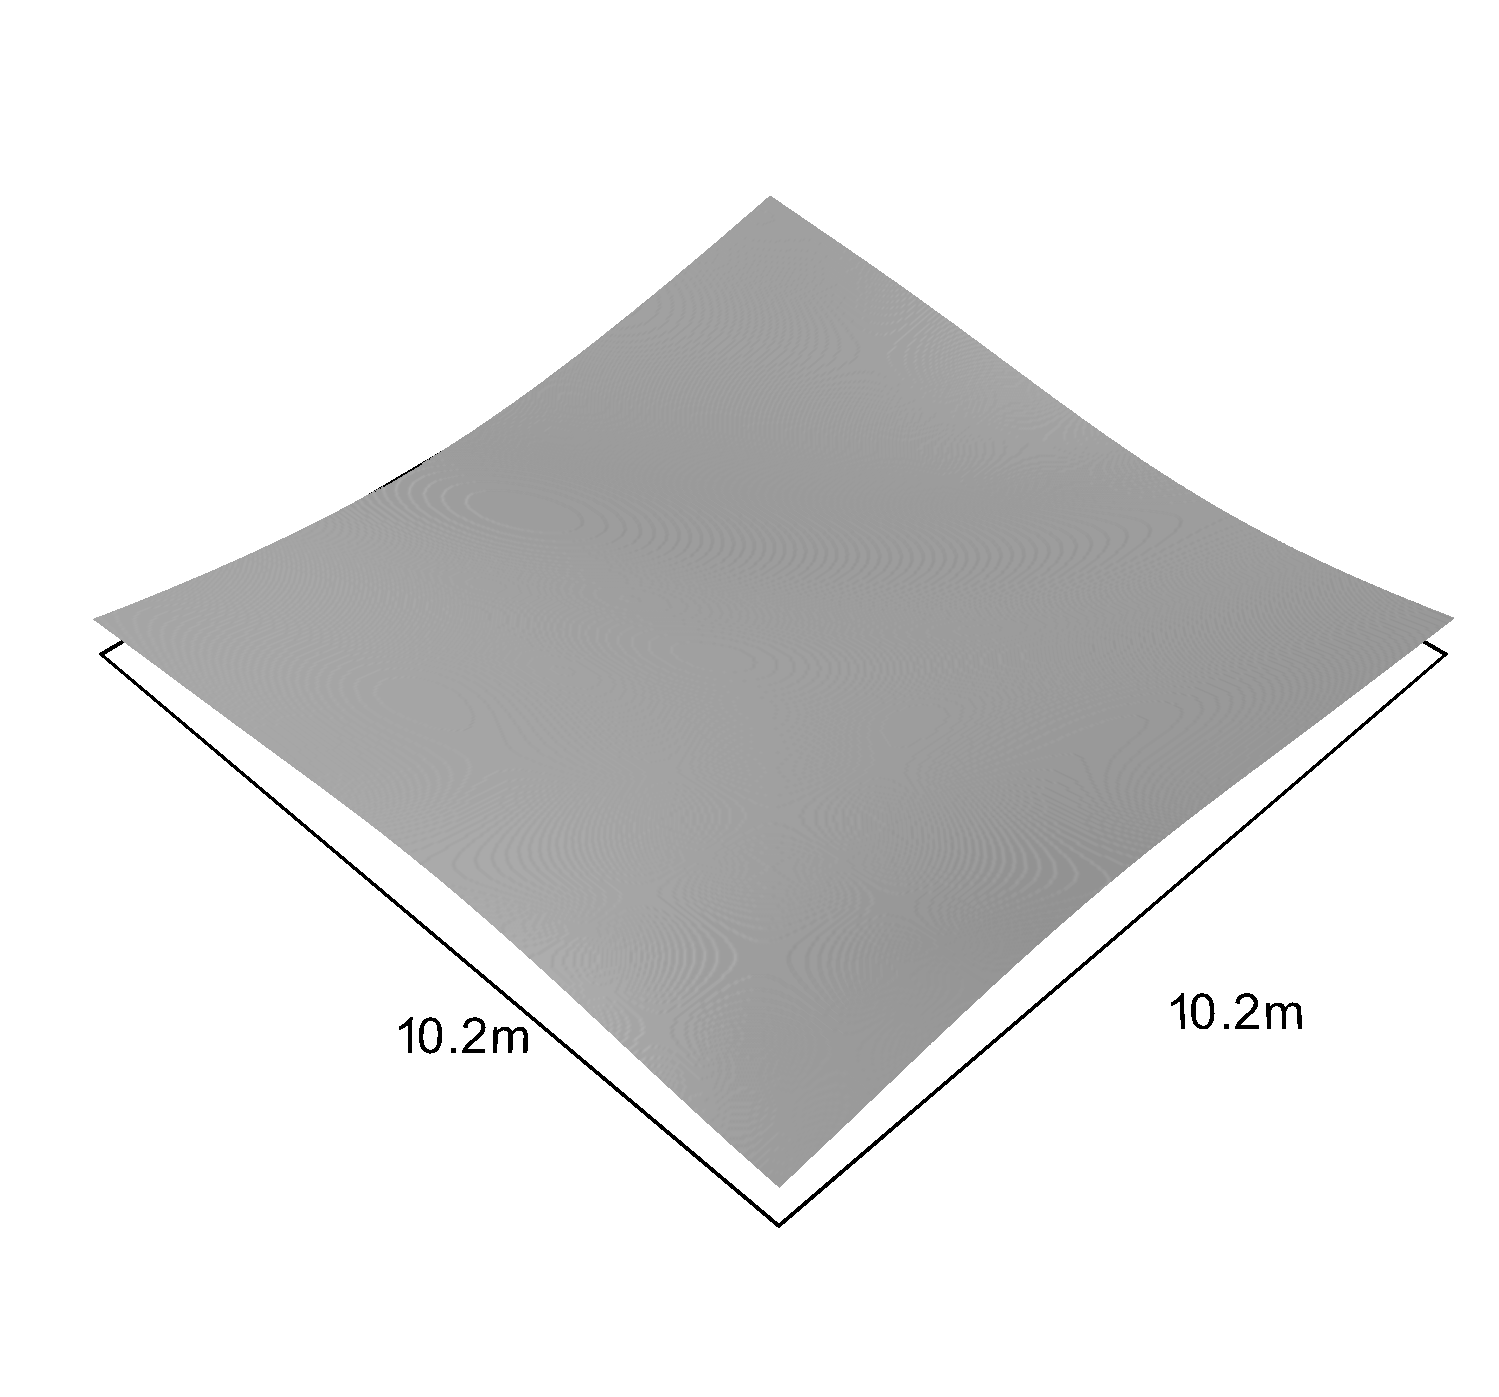
\includegraphics[width=\textwidth]{../img/hm3d_borders/ramp0.png}
            \caption{\emph{ramp0}}
        \end{subfigure}
        \begin{subfigure}[b]{0.23\linewidth}
            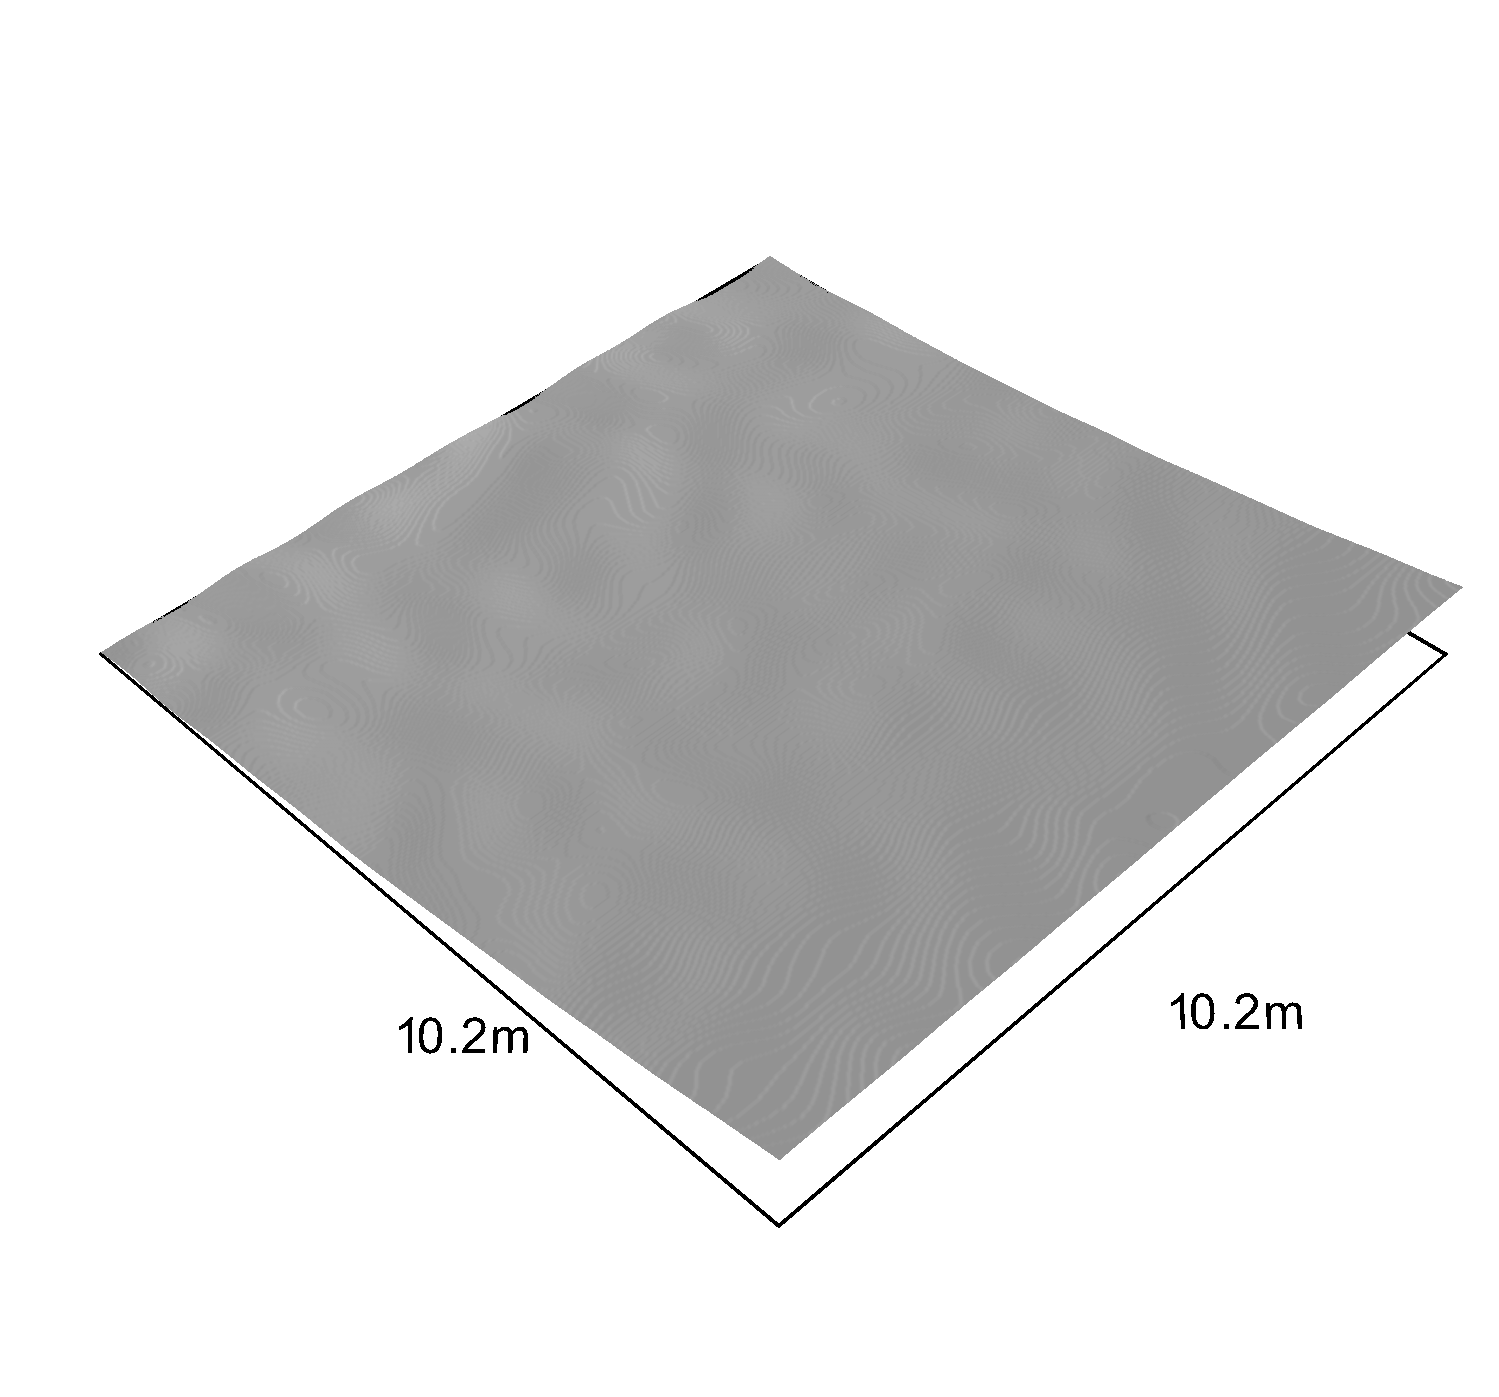
\includegraphics[width=\textwidth]{../img/hm3d_borders/ramp1.png}
            \caption{\emph{ramp1}}
            \end{subfigure}    
          \begin{subfigure}[b]{0.23\textwidth}
            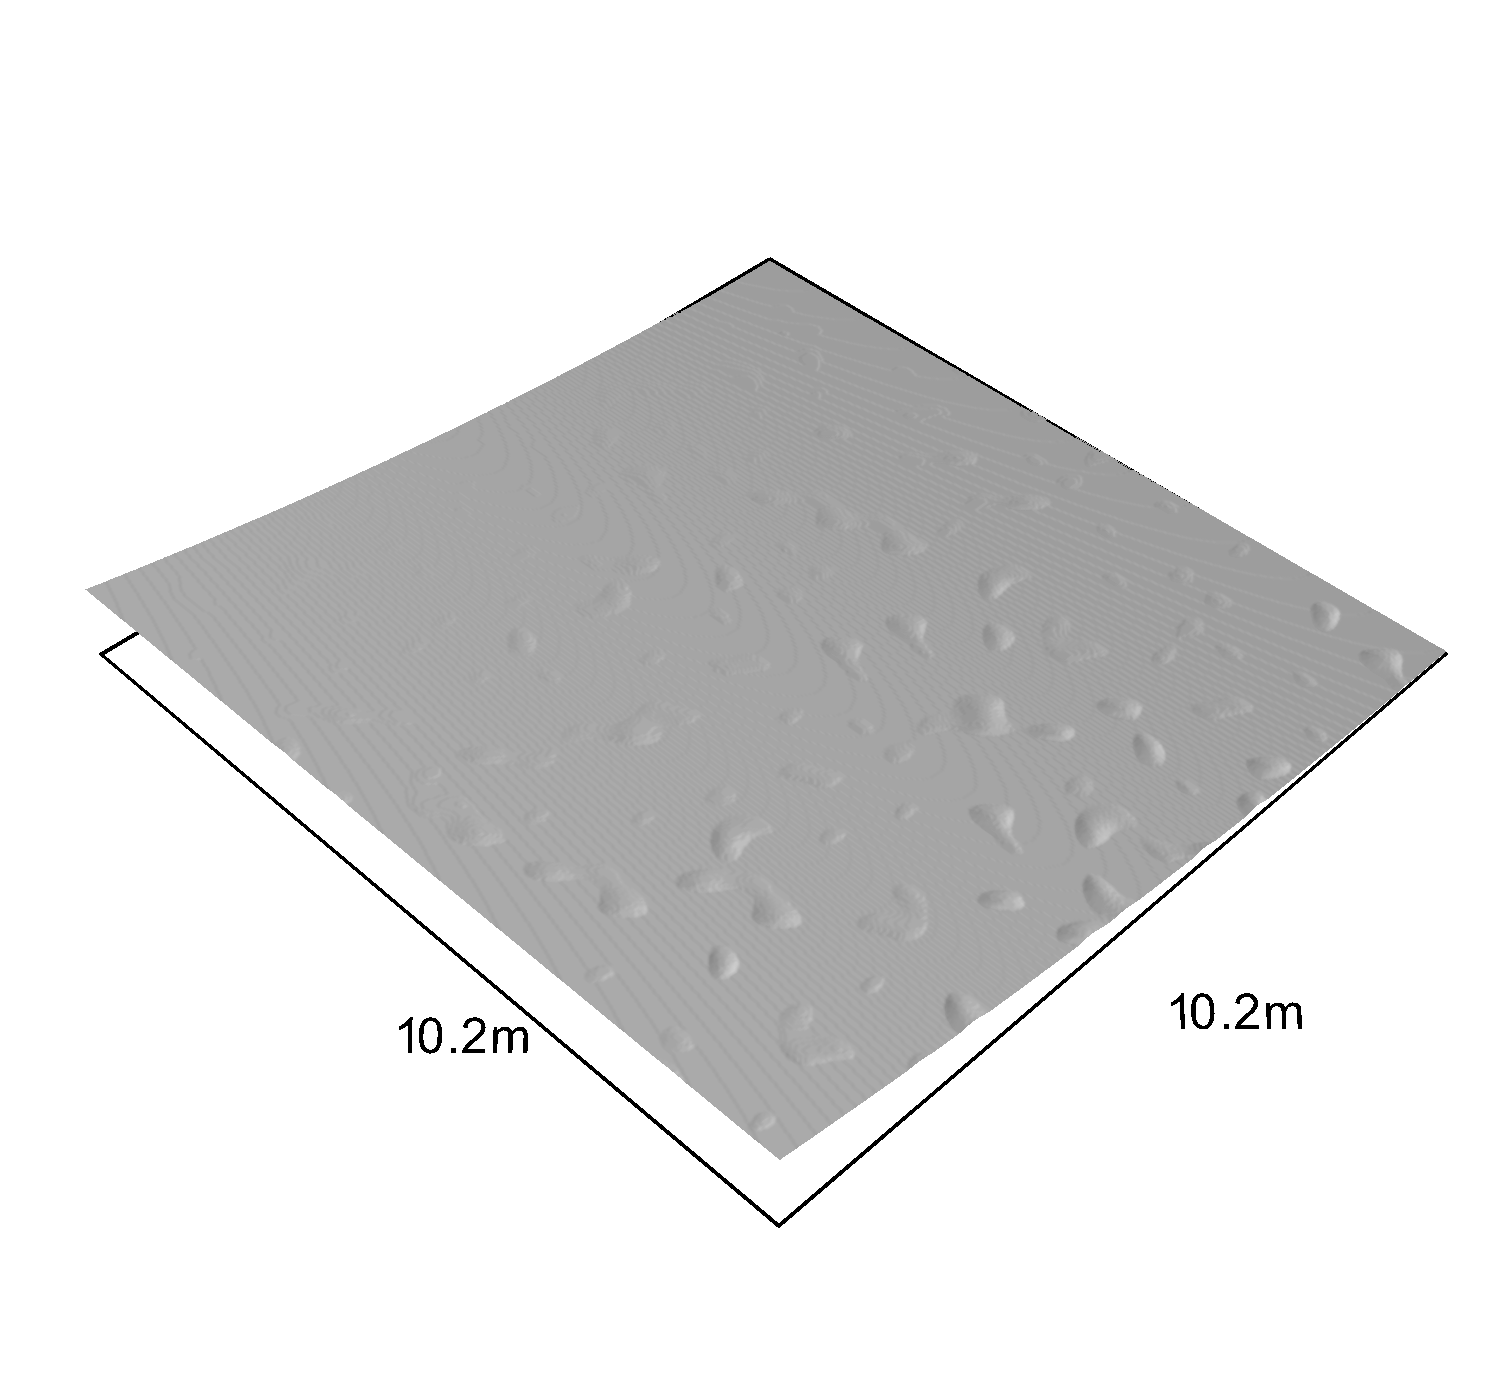
\includegraphics[width=\textwidth]{../img/hm3d_borders/slope_rocks1.png}
            \caption{\emph{slope\_rocks1}}
        \end{subfigure}    
    \caption{Slopes maps.}
\end{figure}
\paragraph{Holes} We also included a map with holes
\begin{figure}[H]
    \centering
        \begin{subfigure}[b]{0.23\textwidth}
            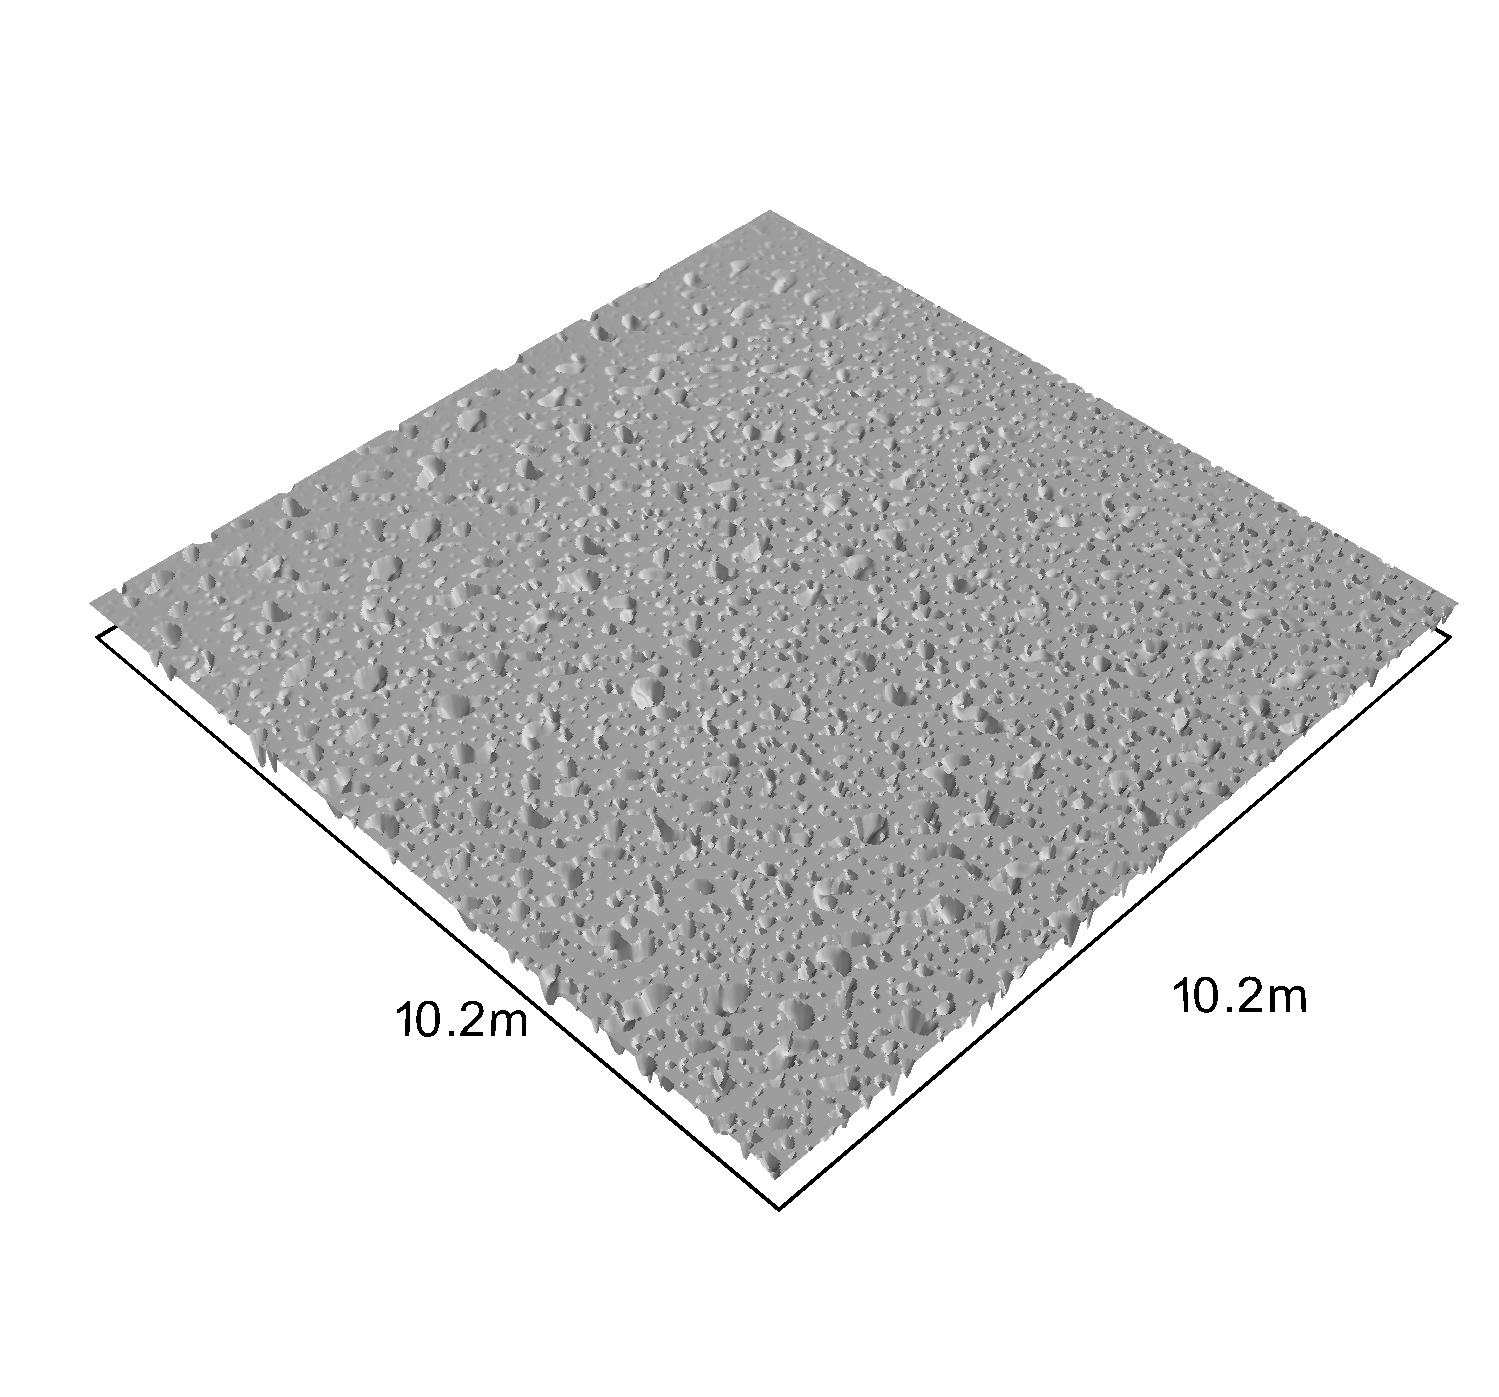
\includegraphics[width=\textwidth]{../img/hm3d_borders/holes1.png}
            \caption{\emph{holes1}}
        \end{subfigure}
\caption{Holes map.}
\end{figure}
\subsection{Real world maps}
We also included real word terrains. We gather two heightmaps produced by ground mapping flying drones from \href{https://www.sensefly.com/education/datasets/}{sensefly}'s dataset, a quarry and a small village. Figure \ref{fig : real-maps} shows the original and a 3D render of the heightmap for each terrain
\begin{figure}[htbp]
    \centering
    \begin{subfigure}[b]{1\textwidth}
    \begin{subfigure}[b]{0.45\textwidth}
        \includegraphics[width=\textwidth]{../img/quarry-real.png}
    \end{subfigure}
    \begin{subfigure}[b]{0.45\textwidth}
        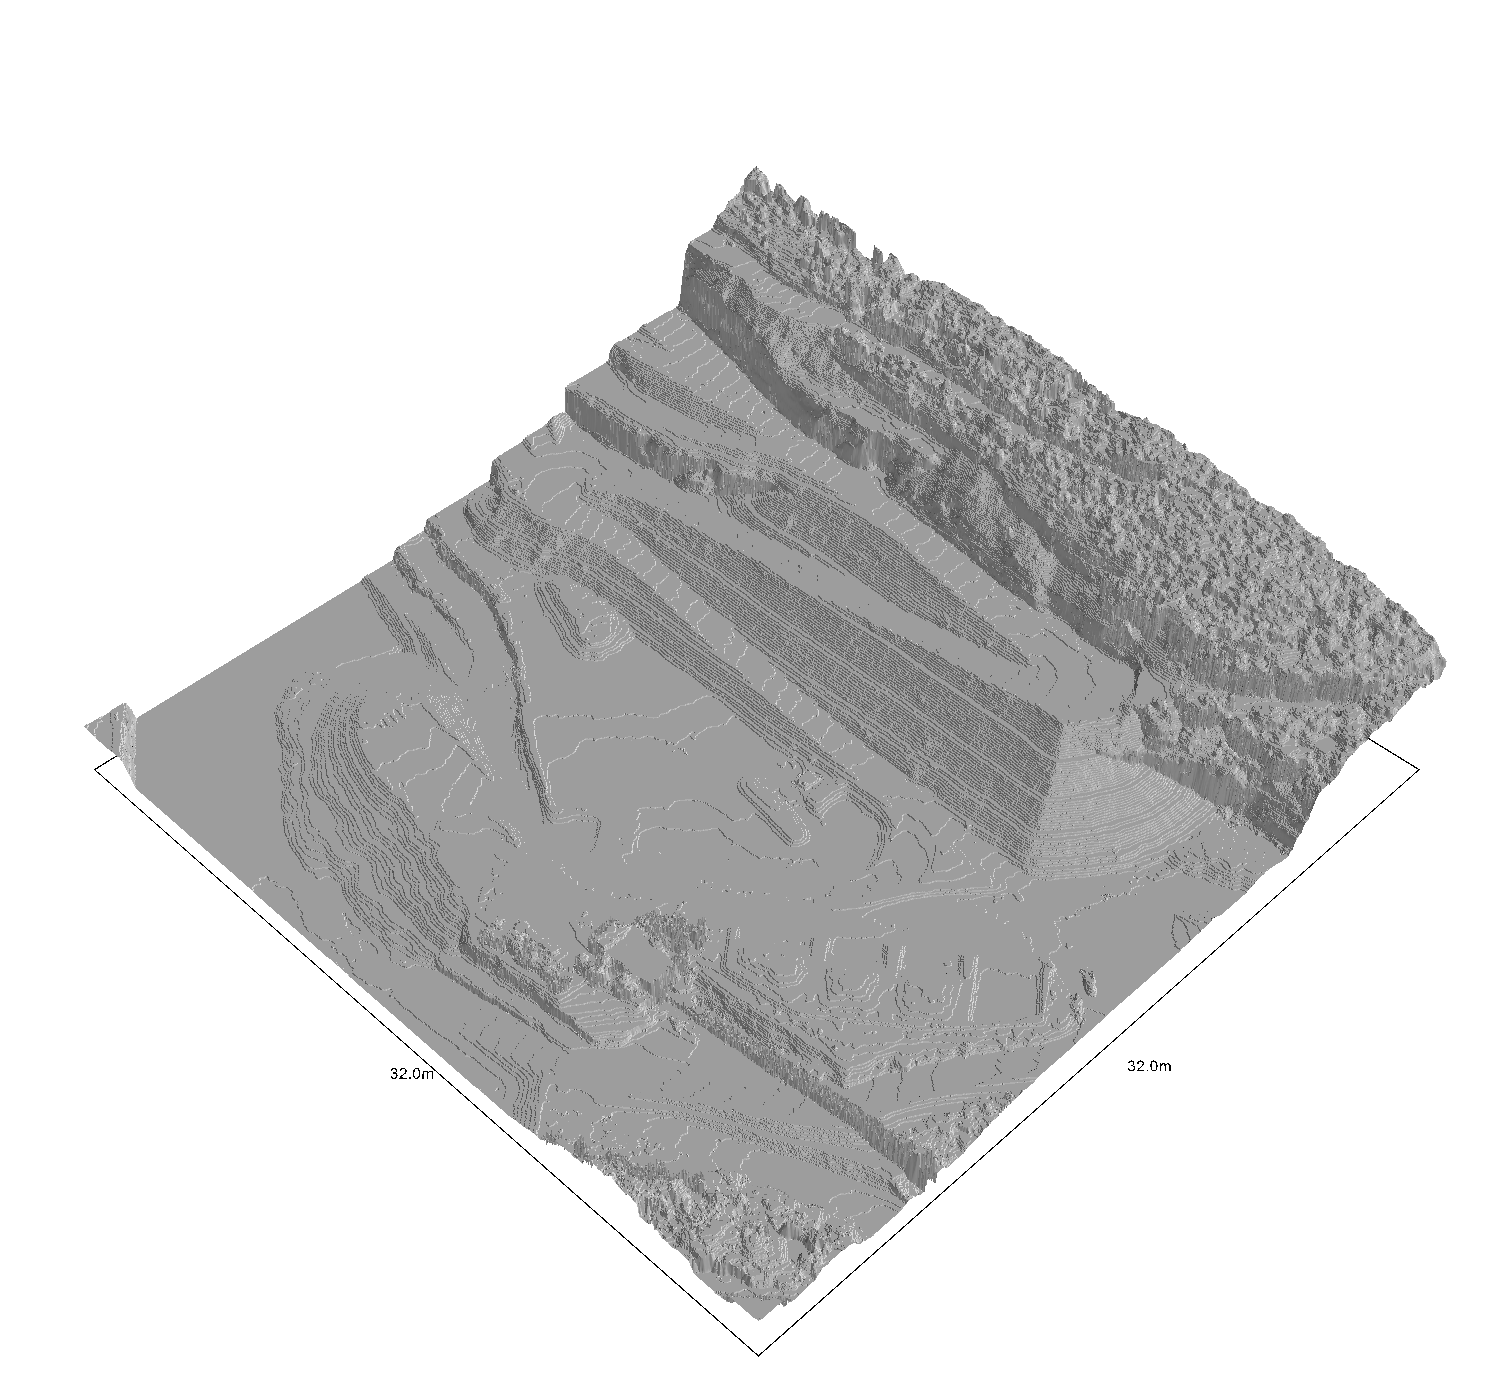
\includegraphics[width=\textwidth]{../img/hm3d_borders/querry-big-10.png}
    \end{subfigure}
    \caption{Quarry}
    \label{fig : real-maps-quarry}
\end{subfigure}
\begin{subfigure}[b]{1\textwidth}
    \begin{subfigure}[b]{0.45\textwidth}
        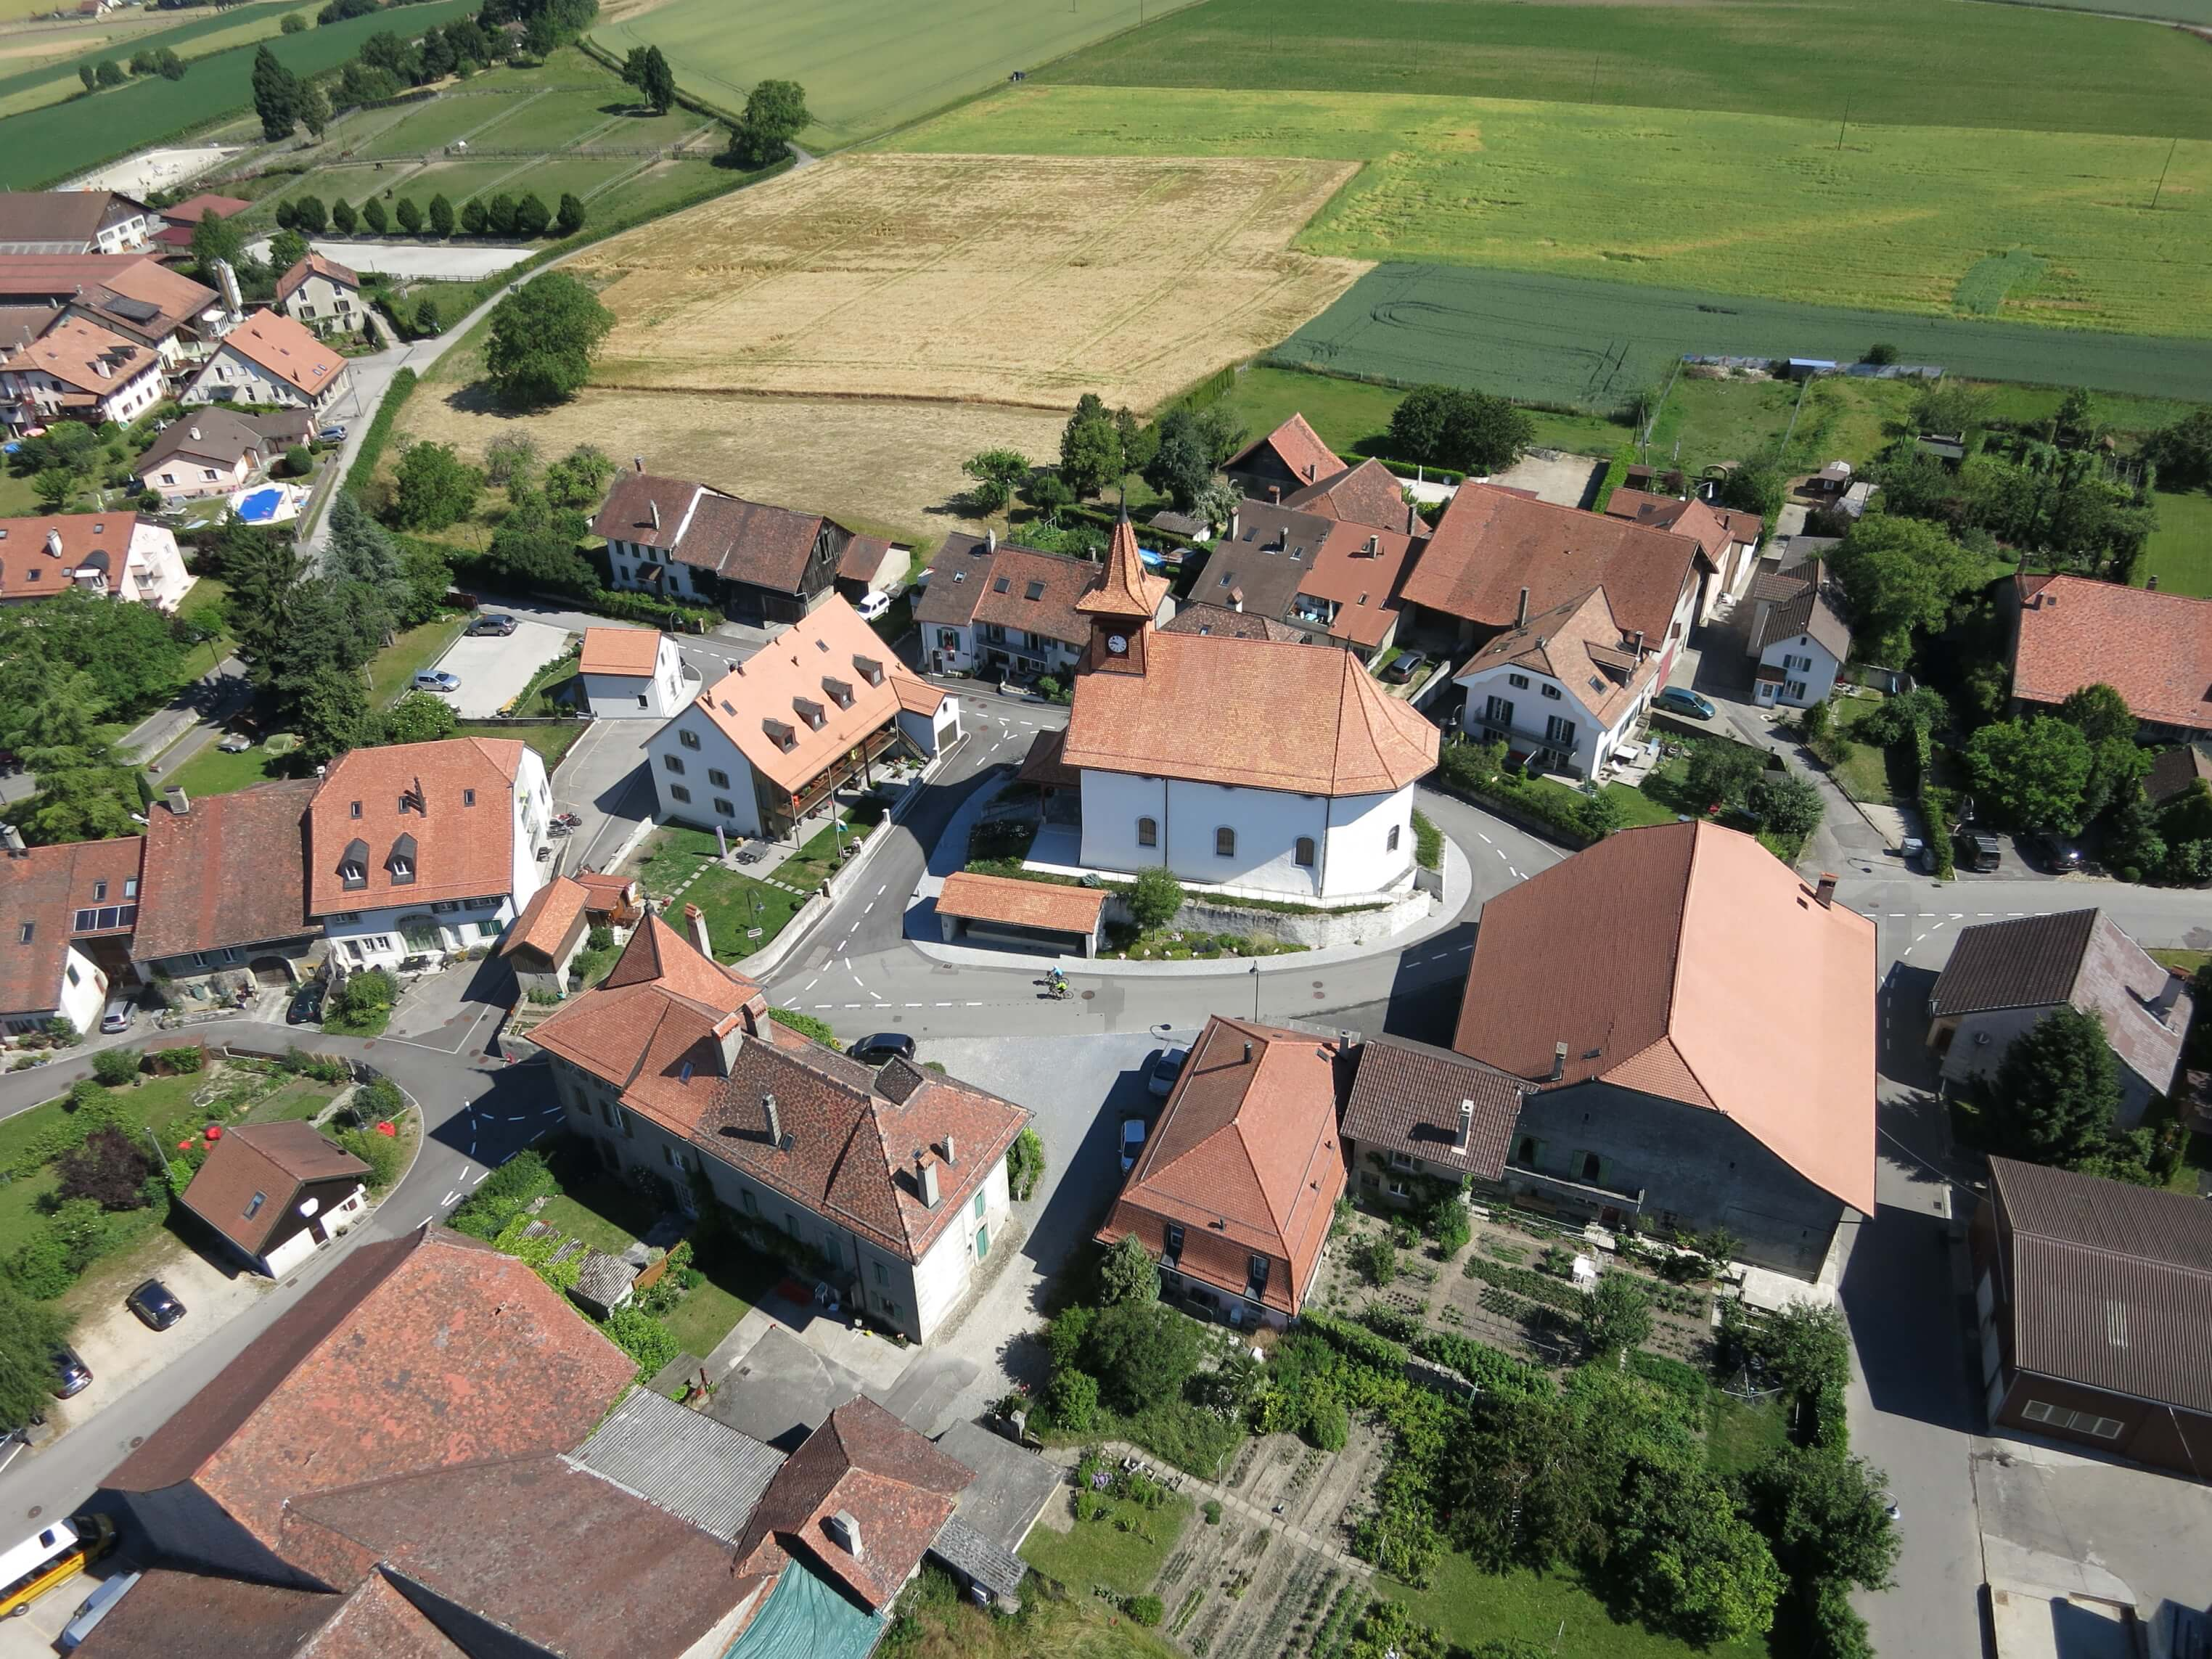
\includegraphics[width=\textwidth]{../img/sullens-real.jpg}
    \end{subfigure}  
    \begin{subfigure}[b]{0.45\textwidth}
        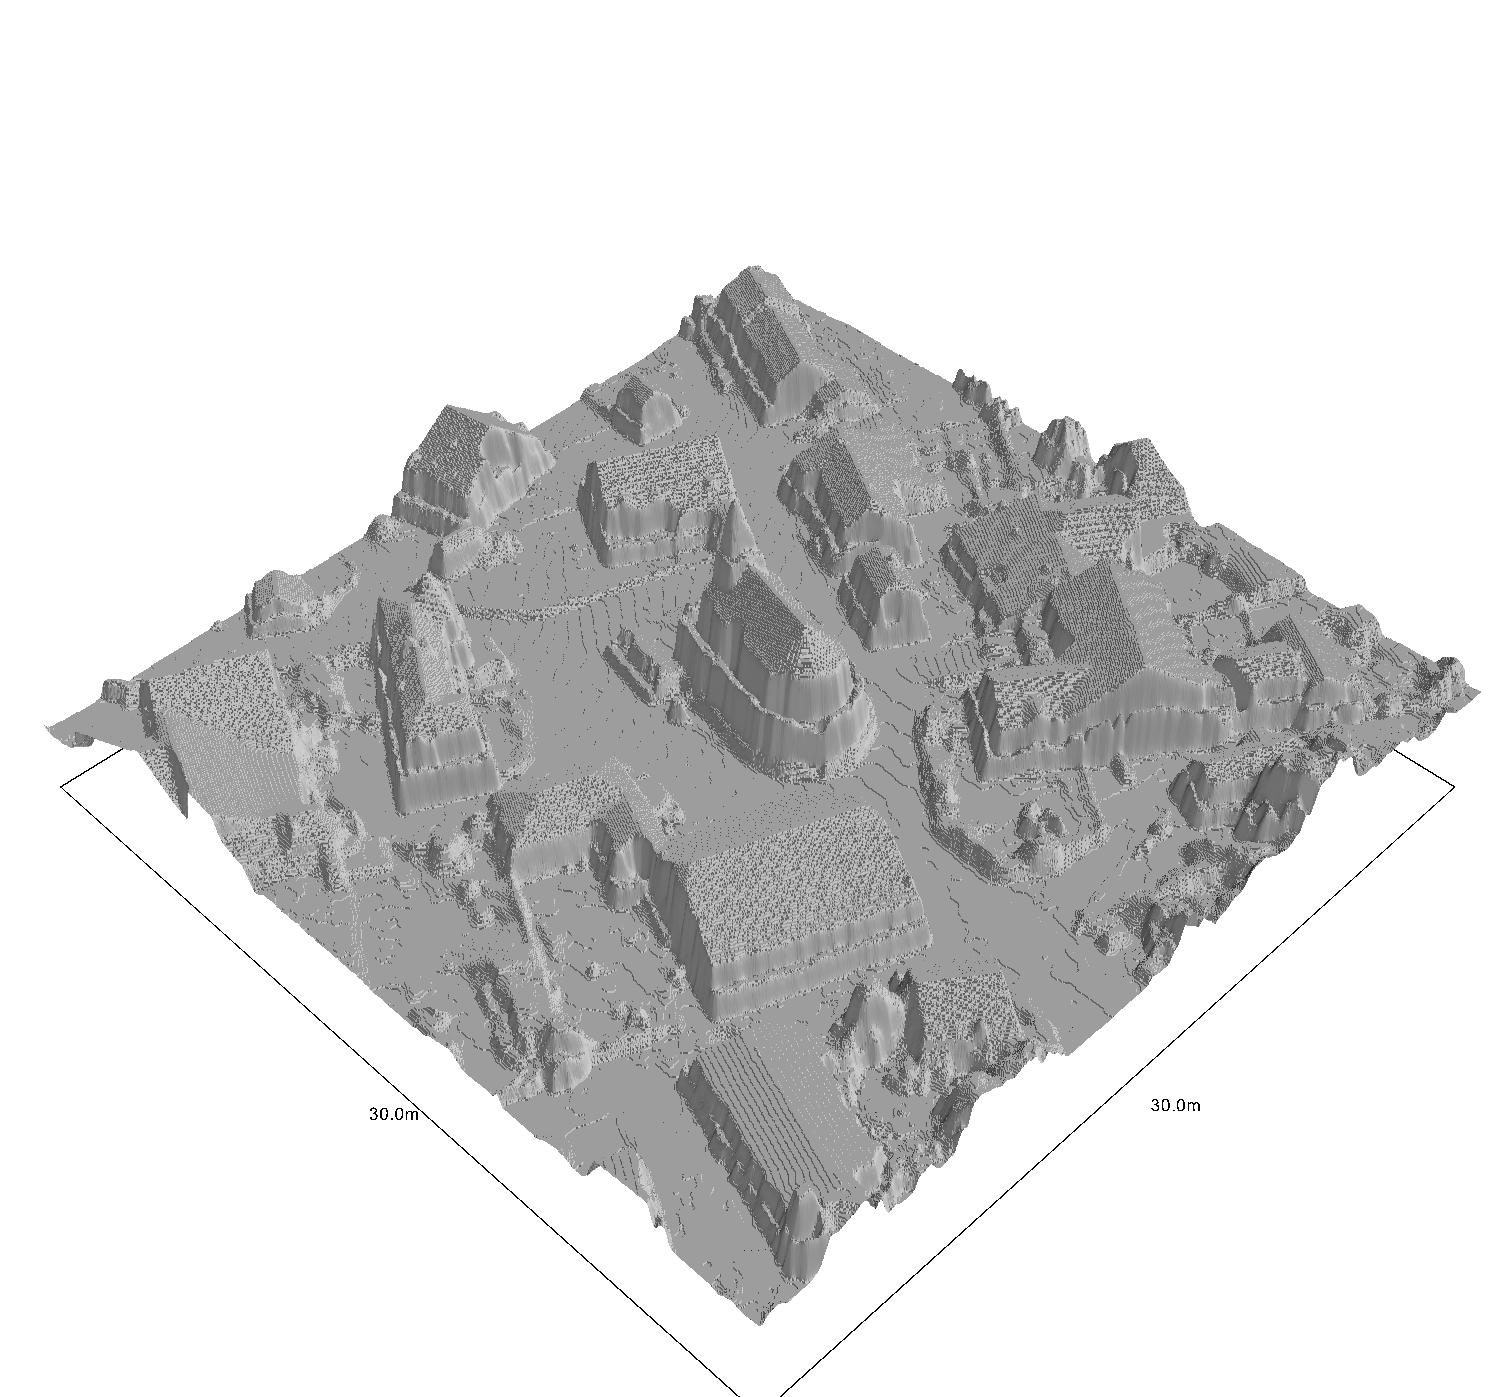
\includegraphics[width=\textwidth]{../img/hm3d_borders/sullens.png}
    \end{subfigure} 
    \caption{A small village.} 
\end{subfigure}
\caption{Real world maps obtained from \href{https://www.sensefly.com/education/datasets/}{sensefly}'s dataset. The left images shows the real world location while on the right a render in 3D of the coresponding heightmaps. Booth images have a maximum height of 10m.}  
\label{fig : real-maps}
\end{figure}

% \subsection{Simulator}
% We used Webots as the simulation plaform for the robot model and the generated terrain. The controller was implemented using the Robotic Operating System, and send data using a special nodes called topics. The controller implements a ROS' node to publish Krock status including its pose at a rate of $250hz$. We decided to reduce it to $50hz$ by using ROS build it \texttt{throttle} command. 
% To load the map into the simulator, we fist had to convert it to Webots's \emph{.wbt} file. Unfortunately, the simulator lacks support for heightmaps so we had to use a script to read the image and perform the conversion. To communicate with the simulator, Webots exposes a wide number of ROS services, similar to HTTP endpoints, with which we can communicate. The client can use the services to get the value of a field of a Webots' Node, for example, if we want to get the terrain height, we have to ask for the field value \texttt{height} from \texttt{TERRAIN} node. In addition, to call one service, we first have to get the correct type of message we wish to send and then we can call it. We decided to implement a little library called \href{https://github.com/FrancescoSaverioZuppichini/Master-Thesis/tree/master/core/utilities/webots2ros}{\texttt{webots2ros}} to hide all the complexity needed to fetch a field value from a node.

% We also implement one additional library called \href{https://github.com/FrancescoSaverioZuppichini/Master-Thesis/tree/master/core/simulation/agent}{\texttt{Agent}} to create reusable robot's interfaces independent from the simulator. The package supports callbacks that can be attached to each agent adding additional features such as storing its interaction. Finally, we used \emph{Gym} \cite{gym}, a toolkit to develop and evaluate reinforcement learning algorithms, to define our environment. Due to the library's popularity, the code can easily be shared with other researches or we may directly experiment with already made RL algorithm in the future without changing the underlying infrastructure.

\section{Simulation}
\subsection{Setup}
We used Webots as the simulation plaform for the robot model and the generated terrains. The controller was implemented using the Robotic Operating System, and send data using a special nodes called topics. The controller implements a ROS' node to publish Krock status including its pose at a rate of $250hz$. We decided to reduce it to $50hz$ by using ROS build it \texttt{throttle} command. 
\subsection{Spawing}
To collect \emph{Krock}'s interaction with the environment, we spawn the robot on the ground and let it move forward for $t$ seconds. We repeat this process $n$ times per each map.
    Unfortunately, spawning the robot is not a trivial task. In certain maps, for instance, \emph{bars1}, a map with tons of walls, we must avoid spawning Krock on an obstacle otherwise the run will be ruined by \emph{Krock} getting stuck at the beginning introducing noise in the dataset. To solve the problem, we defined two spawn strategies, a random spawn and a flat ground spawn strategy. The first one is used in most of the maps without big obstacles such as \emph{slope\_rocks}. This stragety just spawn the robot on random position and rotation. 
    While, the flat ground strategy first selects suitable spawn positions by using a sliding window on the heightmap of size equal Krock's footprint and check if the mean pixel value is lower than a small threshold. If so, we store the center coordinates of the patch as a candidate spawing point. Intuitively, if a patch is flat then its mean value will be close to zero.
Since there may be more flat spawing positions than simulations needed, we have to reduce the size of the candidate points. To maintaing the correct distribution on the map to avoid spawing the robot always in the same cloud of points, we used K-Means with $k$ clusters where $k$ is equal to the number of simulations we wish to run. By clustering, we guarantee to cover all region of the map removing any bias. Picture \ref{fig : spawn-stra} shows this strategy on \emph{bars1}. 
\begin{figure}[htbp]
    \begin{subfigure}[b]{0.45\textwidth}
        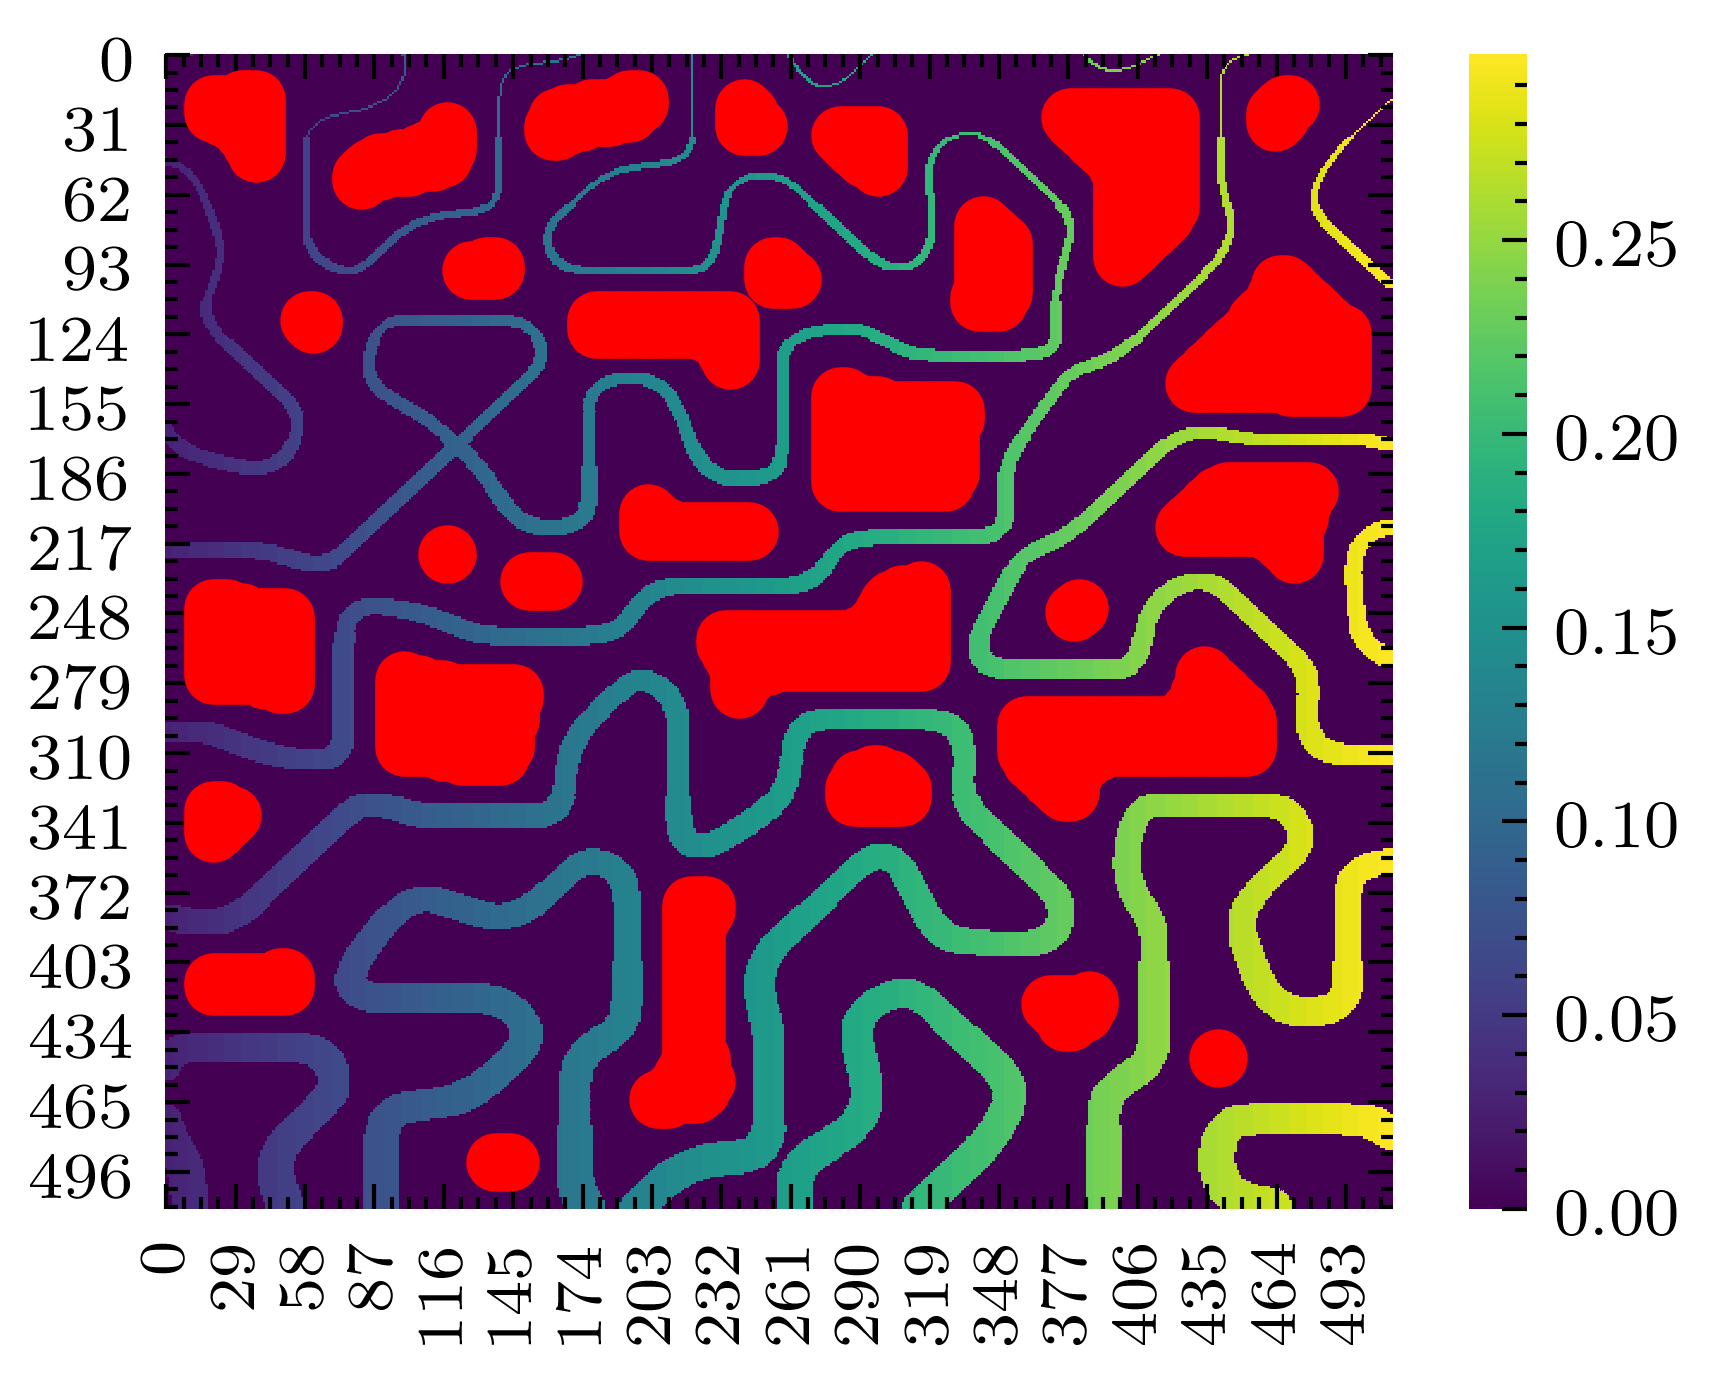
\includegraphics[width=\textwidth]{../img/3/spawn/flat-spawn-10.png}
        \caption{Flat regions}
    \end{subfigure}
    \begin{subfigure}[b]{0.45\textwidth}
        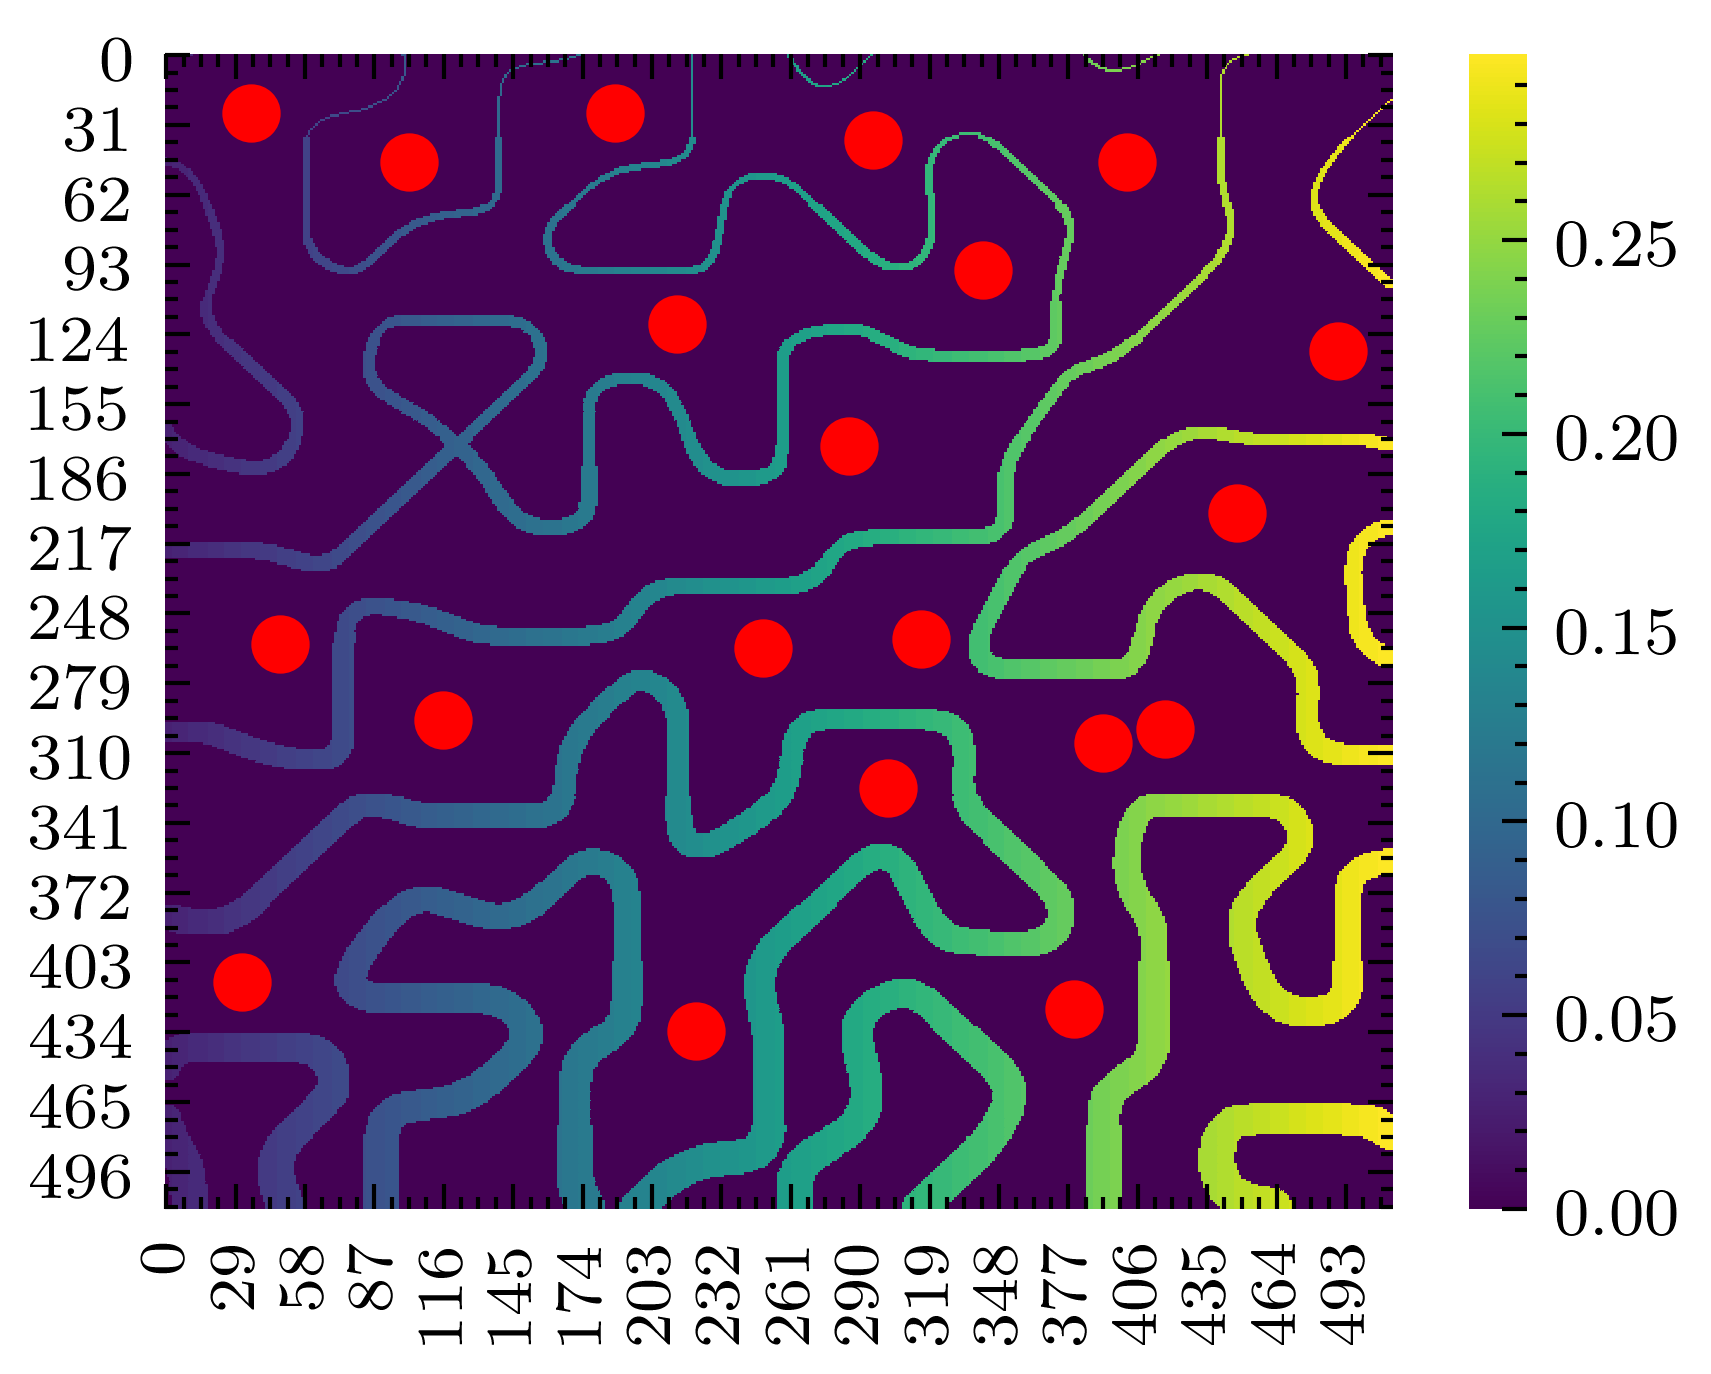
\includegraphics[width=\textwidth]{../img/3/spawn/spawn-10.png}
        \caption{K-Means with $k=20$}
    \end{subfigure}  
\label{fig: spawn-strat}
\caption{Examples of the spawning selection process (marked as red blobs) for the map \emph{bars1} }   
\end{figure}
\subsection{Interactions}
In each simulation, the robot is spawned using the two spawning strategies and it walks forward for a fixed amount of time. We selected ten or twenty seconds depending on the map. Every five simulations we completely regenerate the robot's body to counter possible damages during the hard traversable ground. We moved the robot only forward with a fixed controller since we cannot estimate if the robot can traverse a patch while moving sideways. Table \ref{table: maps} shows the maps configuration used in the simulator. For some map we add three different rocky textures to create more complicated situations. For example, adding some rocks in the ramps map allowed the robot to anchor the legs to the rocks and climb them easily.
\begin{table} [htbp]
    \centering
    \ra{1.2}
    
    \begin{tabular}[]{@{}llcccccc@{}}
      \toprule
      & Map & Height(m) & Spawn & Texture & Simulations & Max time(s) & Dataset \\ 
      \hline
      &\multirow{3}{*}{\emph{bumps0}} & \multirow{3}{*}{2} & \multirow{3}{*}{random} &- & \multirow{3}{*}{50} & \multirow{3}{*}{10} & Train \\
      &&&& rocks1 &  &  & Train \\ 
      &&&& rocks2 &  &  & Train \\ 
      \hline
      &\multirow{3}{*}{\emph{bumps1}} & \multirow{3}{*}{1} & \multirow{3}{*}{random}& - & \multirow{3}{*}{50} & \multirow{3}{*}{10} & Train \\
      &&&& rocks1 &  &  & Train \\ 
      &&&& rocks2 &  &  & Train \\ 
      \hline
      &\multirow{4}{*}{\emph{bumps2}} & \multirow{3}{*}{1} & \multirow{4}{*}{random} &- & \multirow{3}{*}{50} & \multirow{4}{*}{10} & Train \\
      &&&& rocks1 &  &  & Train \\ 
      &&&& rocks2 &  &  & Train \\ 
      && 2 && - &  &  & Train \\ 
      \hline
      &\multirow{3}{*}{\emph{bumps3}} & \multirow{3}{*}{1}& \multirow{3}{*}{random} & - & \multirow{4}{*}{50} & \multirow{3}{*}{10} & Train \\
      &&&& rocks1 &  &  & Train \\ 
      &&&& rocks2 &  &  & Train \\ 
      \hline
      &\emph{steps1} & 1 &random & - & 50 & 10 & Train \\
      \hline
      &\emph{steps2} & 1 &flat & - & 50  &  10& Train \\
      \hline
      &\emph{steps3} & 1 &random & - & 50  &  10& Train \\
      \hline
      &\emph{rails1} & 1 & flat & - & 50 & 20 & Train \\
      \hline
      &\emph{rails2} & 1 && flat & - & 10 & Train \\
      \hline
      &\emph{rails3} & 1 &&  flat&  - & 10 & Train \\
      \hline
      &\multirow{2}{*}{\emph{bars1}} & 1 & \multirow{2}{*}{flat} & - & \multirow{2}{*}{50} & \multirow{2}{*}{10} & Train \\
      && 2 &  & - &  &  & Train \\
      \hline
      &\emph{bars3} & 1 & flat  & - &  &  & Train \\
      \hline
      &\multirow{2}{*}{\emph{ramp0}} & \multirow{2}{*}{1} & \multirow{2}{*}{random} & rocks1 & 50 & \multirow{2}{*}{10} & Train \\
      &&&& rocks2 & 50 &  & Train \\
      \hline
      &\multirow{3}{*}{\emph{ramp1}} & 3 & \multirow{3}{*}{random} & \multirow{3}{*}{-} & \multirow{3}{*}{50} & \multirow{3}{*}{10} & Train \\
      && 4 &&&& & Train \\
      && 5 &&&& & Train \\
      \hline 
      &\multirow{3}{*}{\emph{slope\_rocks1}} & 3 & \multirow{3}{*}{random} & \multirow{3}{*}{-} & \multirow{3}{*}{50} & \multirow{3}{*}{10} & Train \\
      && 4 &&&& & Train \\
      && 5 &&&& & Train \\
      \hline
      &\emph{holes1} & 1 &random & - & 50 & 10 & Train \\
      \hline
      &\emph{quarry} & 10 &random & - & 50 & 10 & Test \\
      \hline
      &\emph{arc rocks} & 1 &random & - & 50 & 10 & Evaluation \\
      \hline
      &&& Total: 1650 & & \\ 
      \bottomrule   
    \end{tabular}
    \label{table: maps}
    \caption{Maps configuration used in the simulator.}
  \end{table}
\section{Postprocessing}
To generate the dataset, we need to extract we had to extract the patches at each robot's pose of the trajectory generated at simulation time. Figure \ref{fig : postprocessing-pipeline} shows each step in the postprocess pipeline.
\begin{figure}[htbp] 
\centering
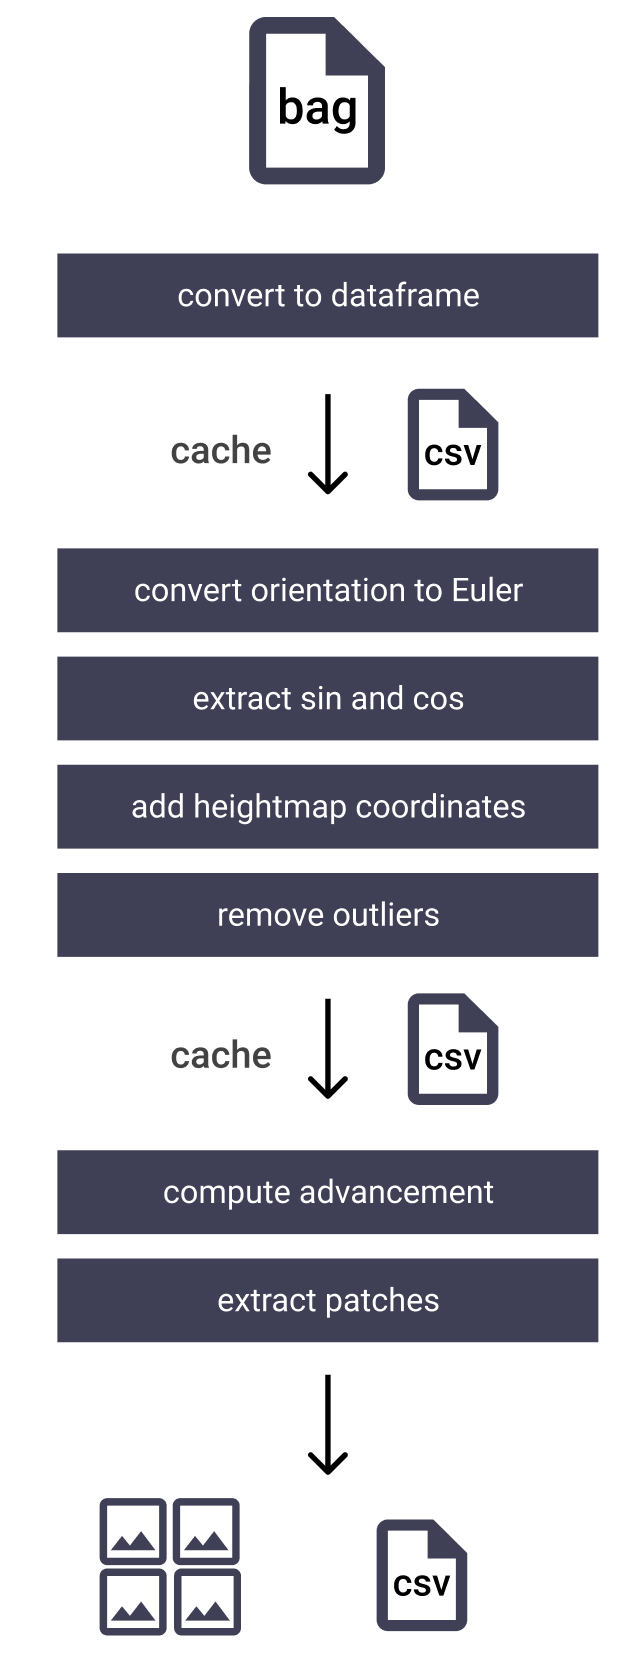
\includegraphics[width=0.66\textwidth]{../img/postprocessing-pipeline.png}
\caption{Postprocessing pipeline flow graph, starting from the top.}
\label{fig: postprocessing-pipeline}
\end{figure}
\subsection{Parse trajectories}
First, we converted the robot's trajectories, stored as \emph{.bag} files, to a more convenient data structure, pandas' dataframes. Them, we cache them into \emph{.csv} files. This operation is done only once.
% We used \href{https://github.com/aktaylor08/RosbagPandas}{\texttt{rosbag\_pandas}}, an open source library we ported to python3, to perform the conversion.
% This 
After, we loaded the stored dataframes with the respective terrains and start the data cleaning process. We removed the the first second of the simulation time to account for the robot spawning time. Then, we eliminated all the entries where a part of Krock was outside the edges of the map. After the data cleaning process, we converted quaternion rotation to Euler notation using the \href{https://duckduckgo.com/?q=ros+tf&atb=v154-1__&ia=web}{\texttt{tf}} package from ROS. Then, we extracted the $\sin$ and $\cos$ from the Euler orientation last component and stored them in a column. In the simulator, the position $(0,0$ correspond to the center of the map, while on the heightmap, like all images, $(0,0$ is the top left corner. To later crop the the correct region from the map, we needed to convert the robot's position into the heightmap's coordinates. This part is also run once and it is cached to speed up latter runs.

\subsection{Advancement computation}
To compute the robot's advancement we needed to define a time window, $\Delta t$, and consider how much the robot traveled between the currenct pose, $X(t)$ and the future one $X(t + \Delta t)$. We observed from the simulator than the robot moves each leg every second. Thus, we selected a time window of two seconds to allow Krock to move booth legs. 

\subsection{Patch extraction}
Each patch must contain both Krock's footprint, to include the situations where the obstacle is under the robot, and certain amount of ground region in front of it. Intuitively, we want to include in each patch the correct amount of future informations according to the selected time window. Thus, we should add the maximum possible ground that Krock could traverse. 

To find out the correct value, we must compute the maximum advancement on a flat ground for the $\Delta t$ and use it to calculate the final size of the patch. We compute it by running some simulations of \emph{Krock} on flat ground and averaging the advancement getting a value of $70$cm in our $\Delta t = 2$s.

Each patch must include Krock's footprint and the maximum possible distance it can travel is a $\Delta t$. So, since Krock's pose was stored from IMU located in the juncture between the head and the legs, we have to crop from behind its length, $85$cm minus the offset between the IMU and the head, $14$cm. Then, we have to take $70$cm, the maximum advancement with a $\Delta t = 2$s plus the removed offset. The following figure visualizes the patch extraction process. 
\begin{figure}[htbp]
    \centering
    \begin{subfigure}[b]{0.66\textwidth}
        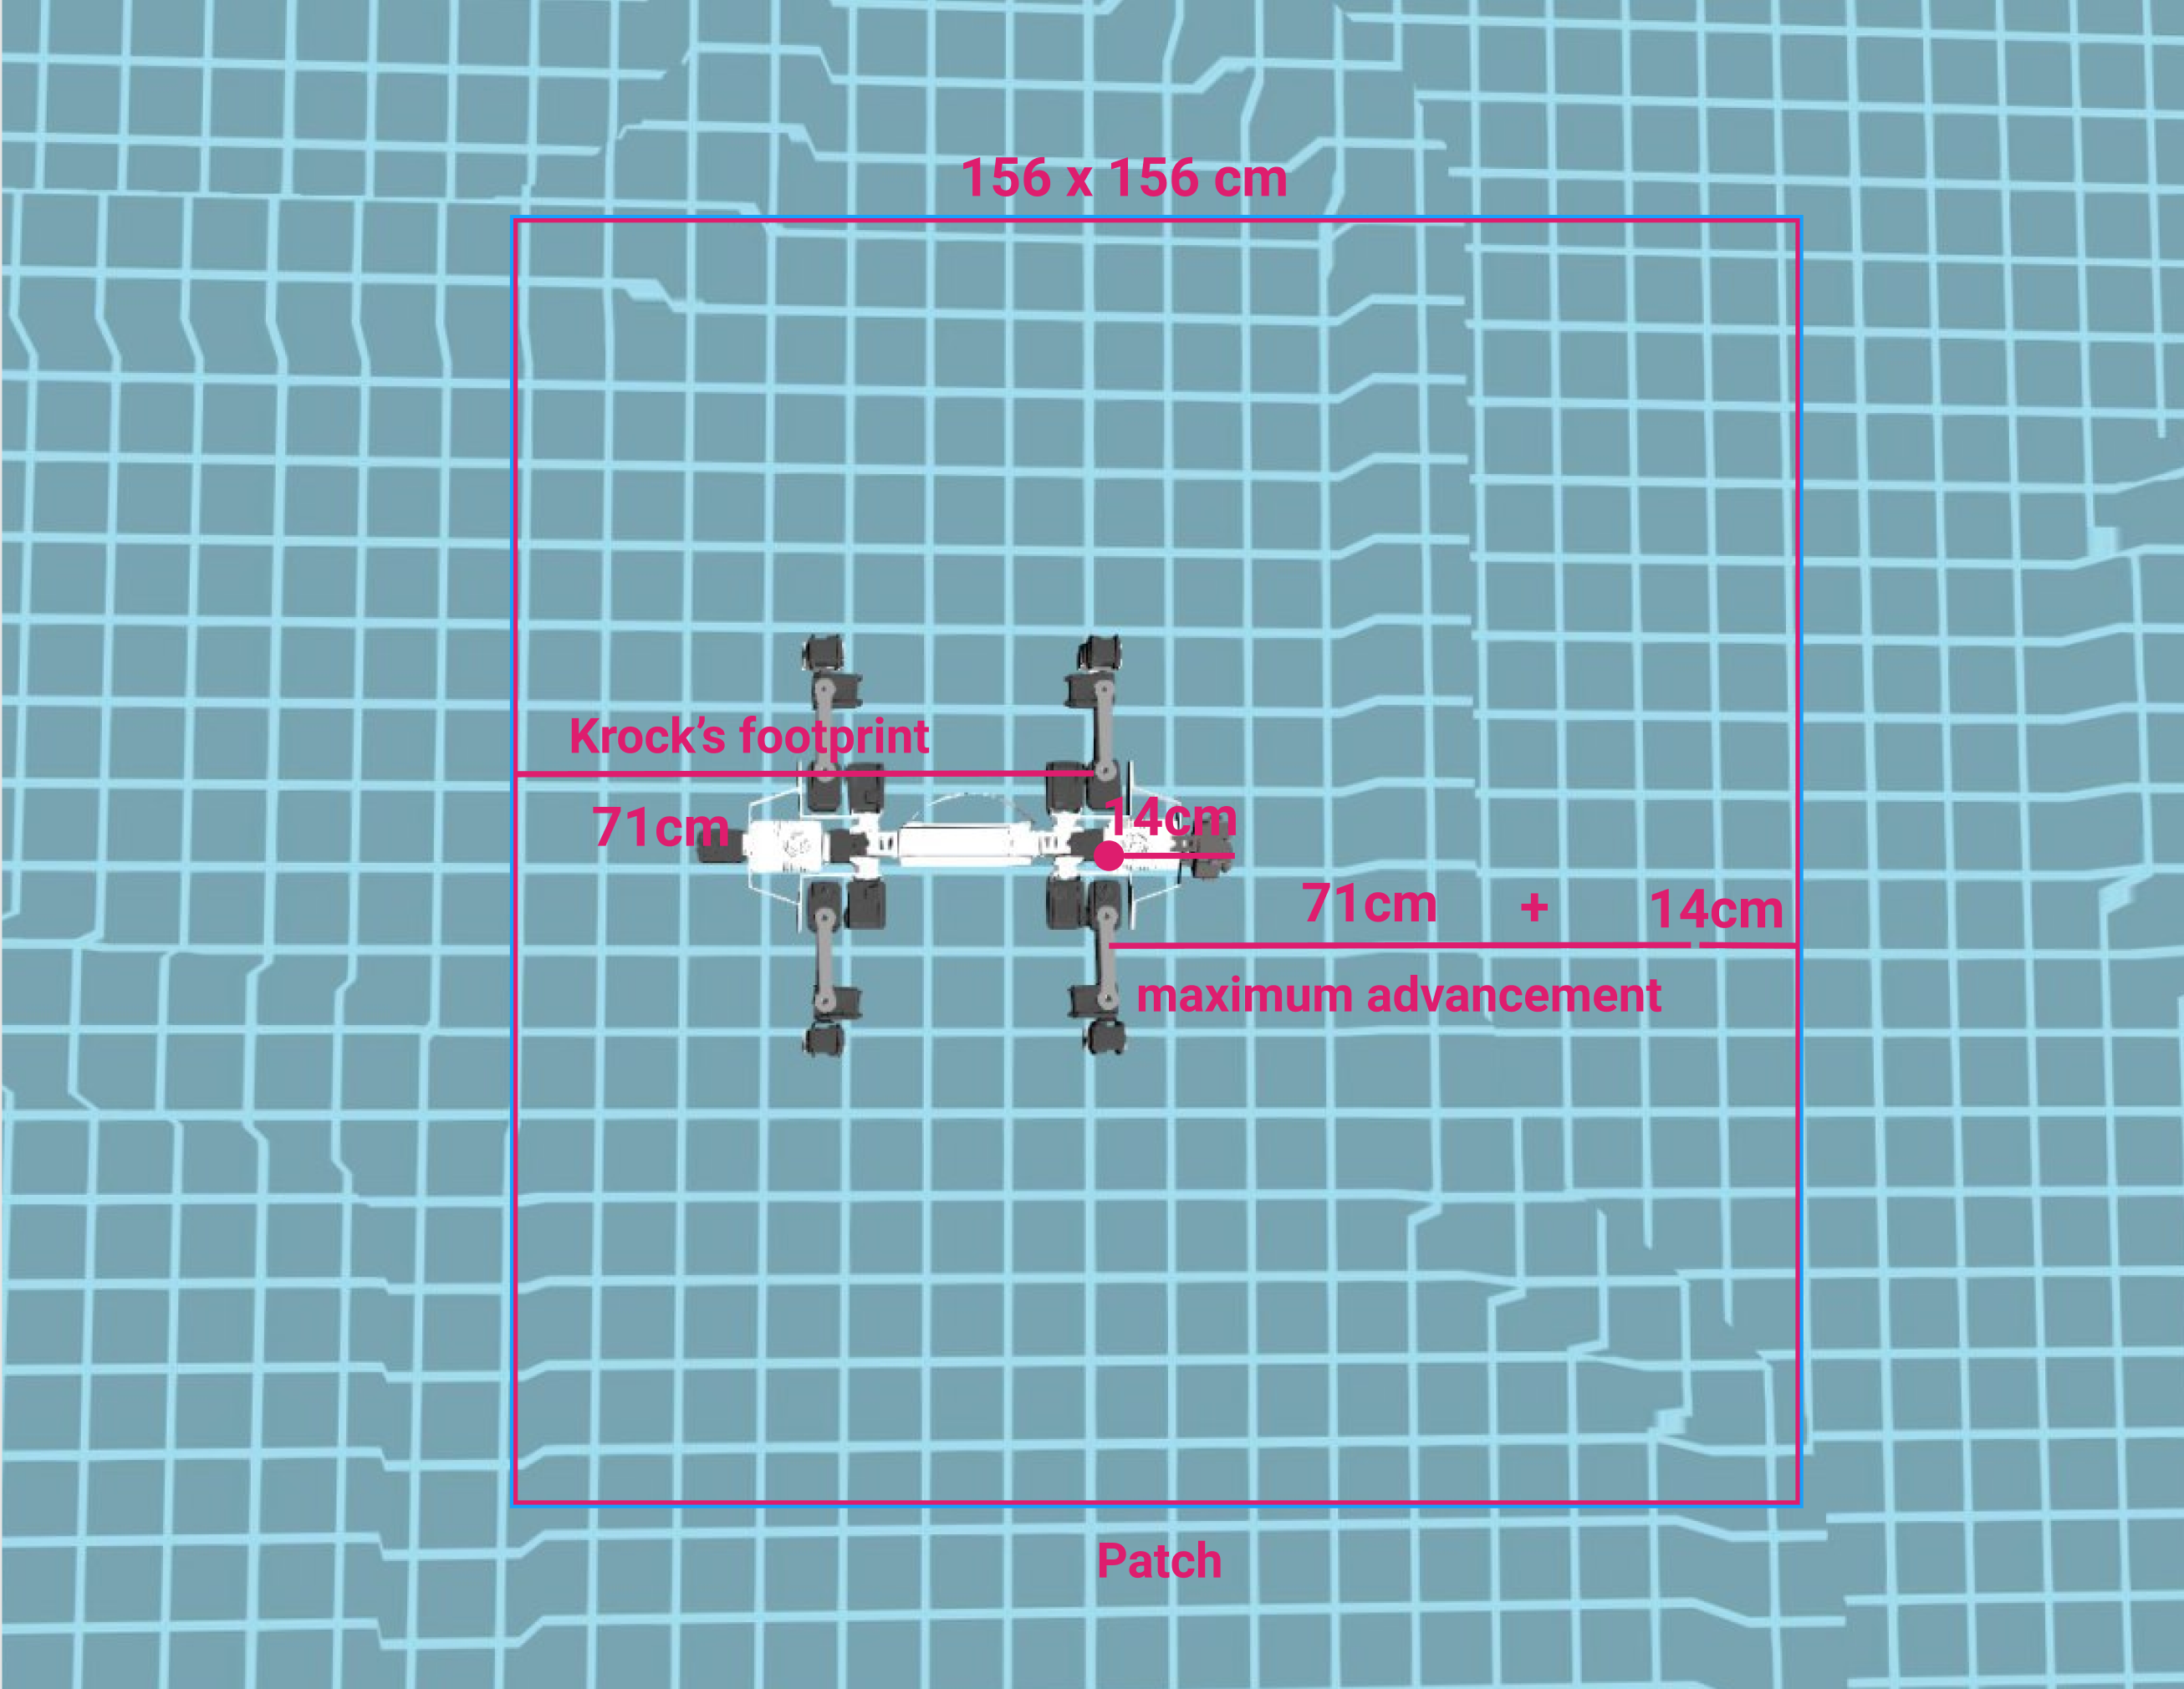
\includegraphics[width=\textwidth]{../img/3/crop/crop.png}
        \caption{Robot in the simulator.}
    \end{subfigure}
    \begin{subfigure}[b]{0.45\textwidth}
        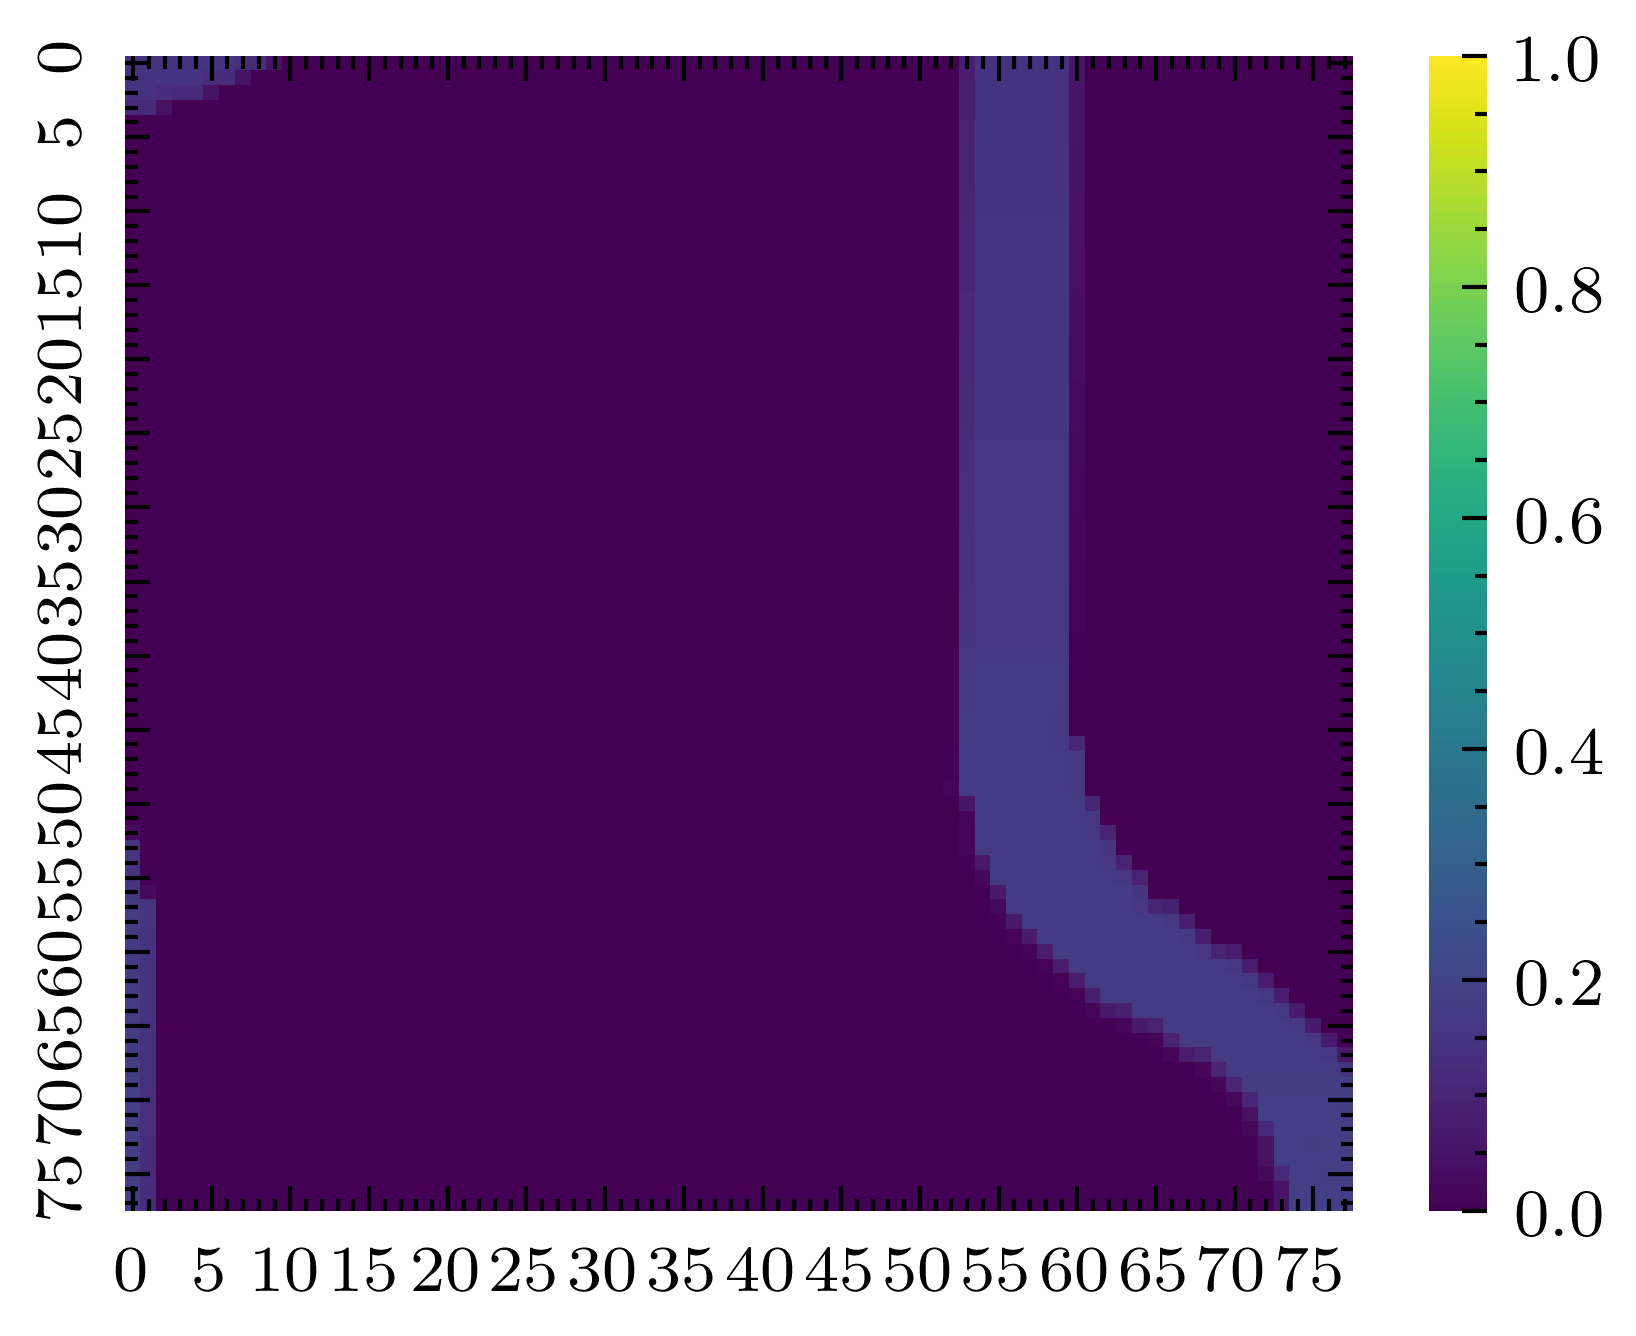
\includegraphics[width=\textwidth]{../img/3/crop/test-1-2d.png}
        \caption{Cropped patch in 2d.}
    \end{subfigure}
    \begin{subfigure}[b]{0.45\textwidth}
        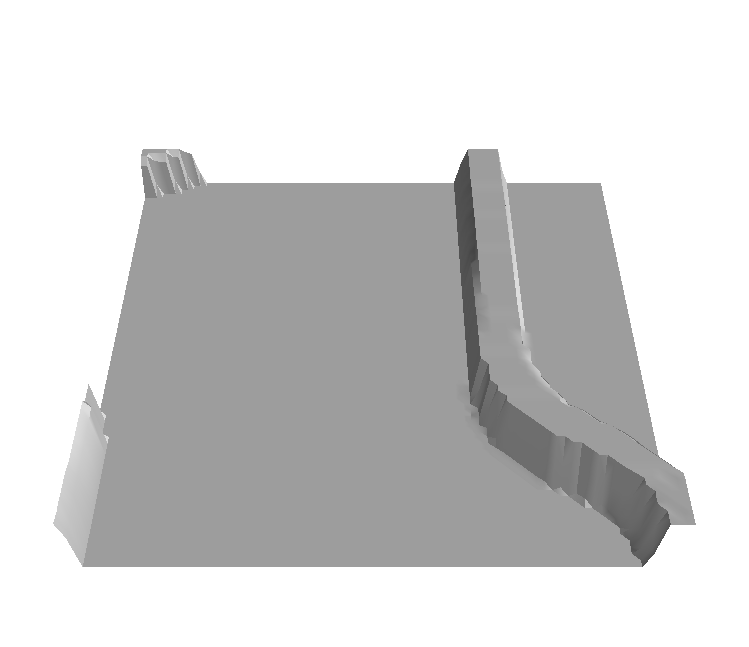
\includegraphics[width=\textwidth]{../img/3/crop/0.png}
        \caption{Cropped patch in 3d.}
    \end{subfigure}
\caption{Patch extraction process for $\Delta t = 2$s.}   
\end{figure}
Lastly, we create a final dataframe containing the map coordinates, the advancement, and the patches paths for each simulation and store them to disk as \emph{.csv} files. 

\subsection{Final dataset}
The final dataset is composed by $\approx 450$K and $\approx 37$K patches for the train and test set respectively. We also generated $\approx 38$K patches using the \emph{arc rocks} map to further evaluate the model. The whole pipeline took less than one hour to run the first time with 16 threads, and, once it is cached, less than fifteen minutes to extract all the patches. To compleness, we plotted in figure \ref{ mean-advs-train} the mean advancement over each map in the traning set. 
\begin{figure}[htbp]
    \centering
    \includegraphics[width=\linewidth]{../img/datasets/box_for_each_map.png}
    \caption{Advancement on each map with a $\Delta t = 2$s in ascendent order.}
    \label{fig : mean-advs-train}
\end{figure}
As sanity check, we visualized some of the patches from the train set ordered by advancement, to conclude the data generation process was correct. Tigure \ref{fig : train-patches-sample} shows a sample of fourty patches.
\begin{figure}[htbp] 
    \centering
    \begin{subfigure}[b]{0.19\textwidth}
    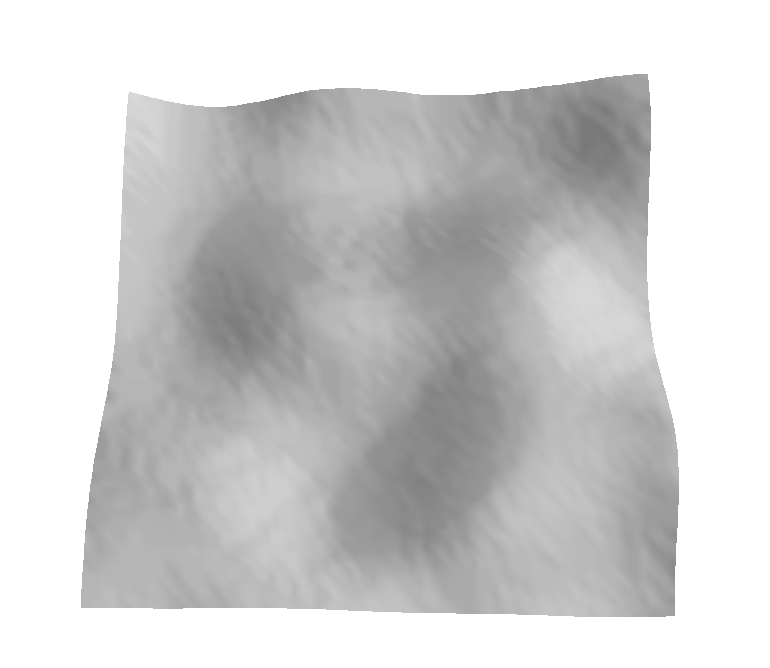
\includegraphics[width=\linewidth]{../img/5/train/all/-1-patch-3d-majavi-3.png}
    \caption{$-1$cm}
    \end{subfigure}
    \begin{subfigure}[b]{0.19\textwidth}
    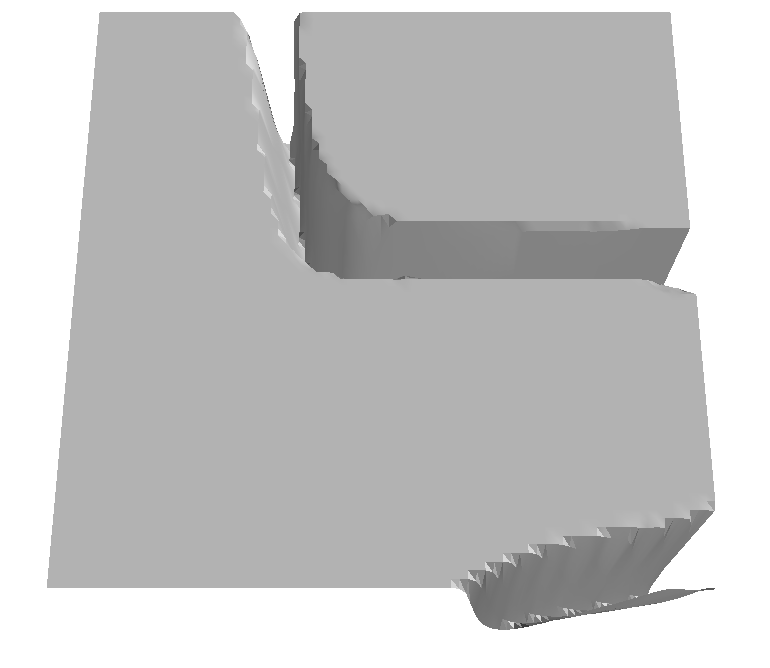
\includegraphics[width=\linewidth]{../img/5/train/all/-3-patch-3d-majavi-2.png}
    \caption{$-3$cm}
    \end{subfigure}
    \begin{subfigure}[b]{0.19\textwidth}
    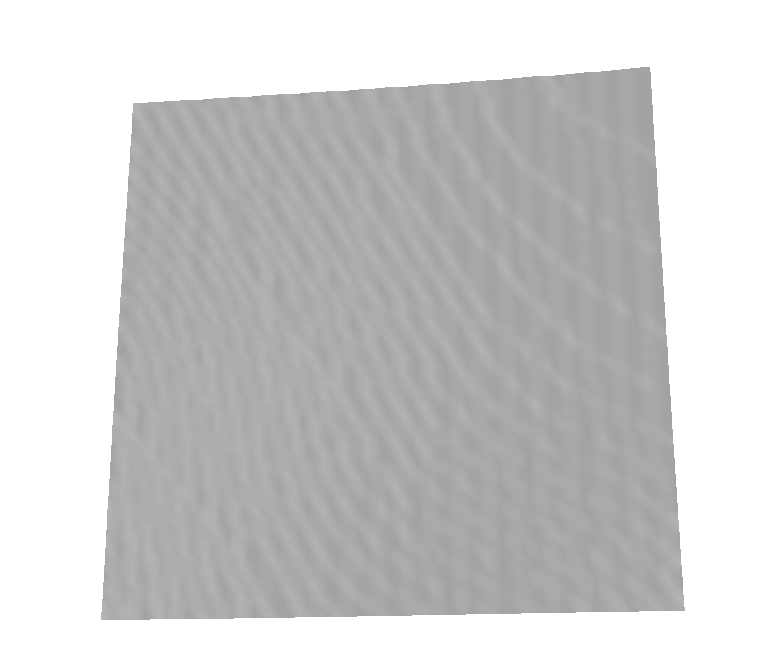
\includegraphics[width=\linewidth]{../img/5/train/all/-372-patch-3d-majavi-0.png}
    \caption{$-3$cm}
    \end{subfigure}
    \begin{subfigure}[b]{0.19\textwidth}
    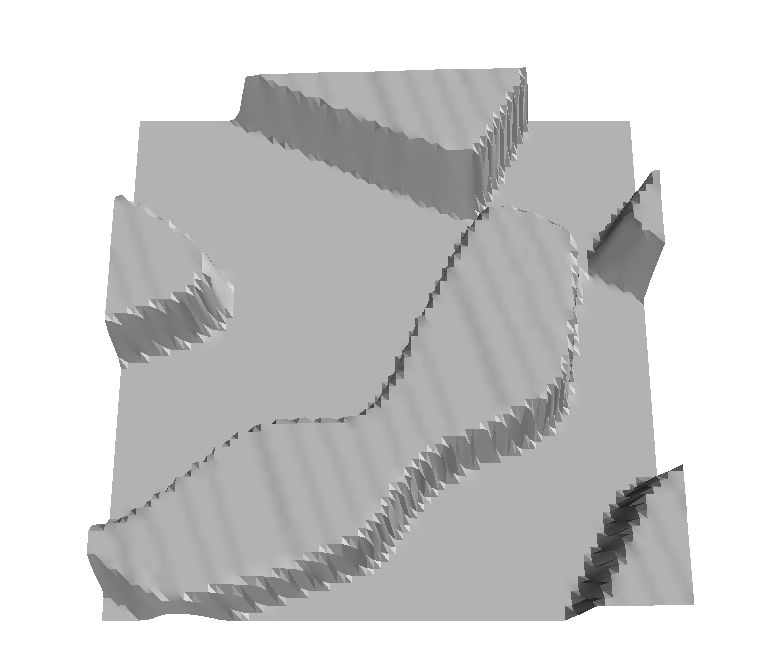
\includegraphics[width=\linewidth]{../img/5/train/all/-6-patch-3d-majavi-1.png}
    \caption{$-6$cm}
    \end{subfigure}
    \begin{subfigure}[b]{0.19\textwidth}
    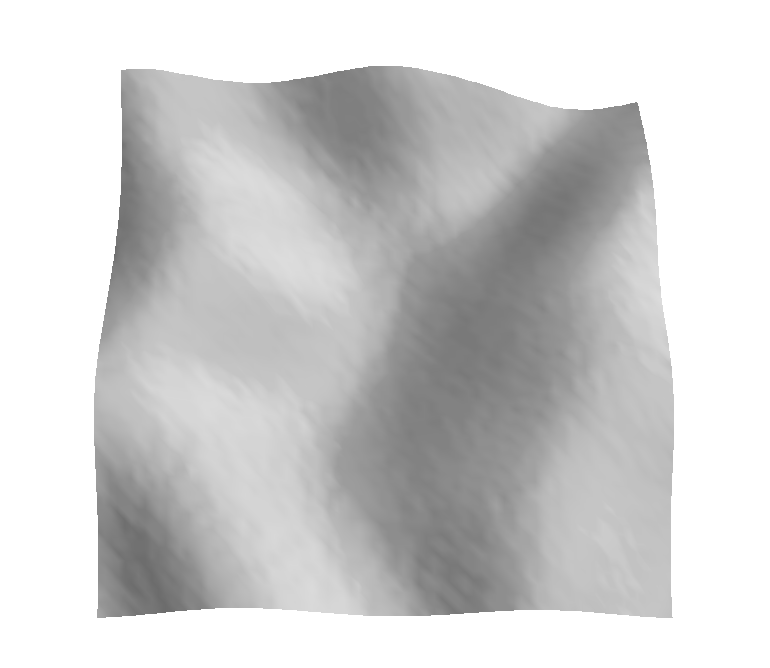
\includegraphics[width=\linewidth]{../img/5/train/all/00-patch-3d-majavi-4.png}
    \caption{$00$cm}
    \end{subfigure}
    \begin{subfigure}[b]{0.19\textwidth}
    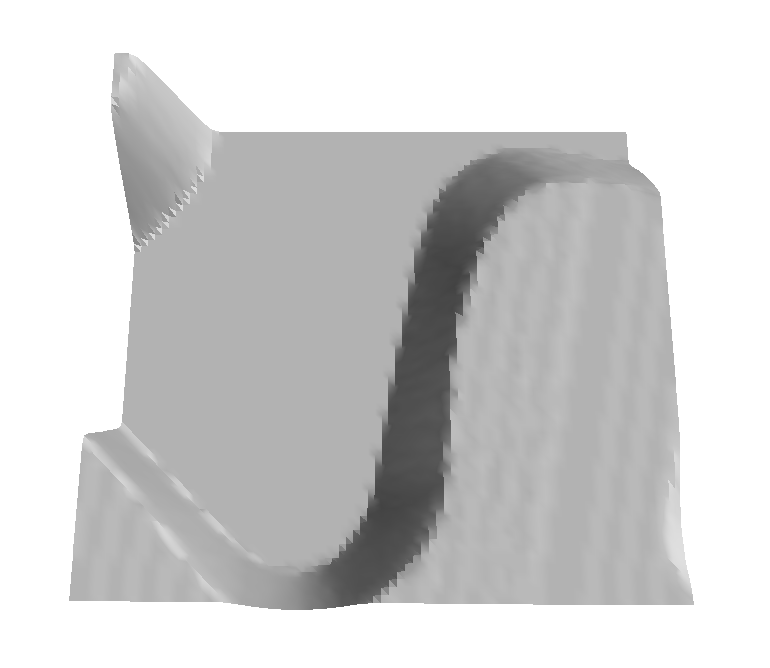
\includegraphics[width=\linewidth]{../img/5/train/all/01-patch-3d-majavi-5.png}
    \caption{$01$cm}
    \end{subfigure}
    \begin{subfigure}[b]{0.19\textwidth}
    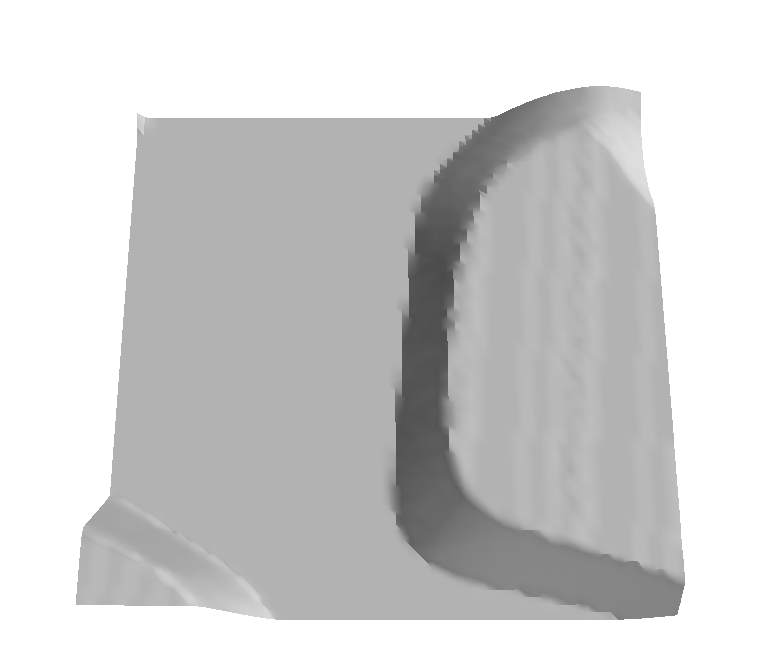
\includegraphics[width=\linewidth]{../img/5/train/all/02-patch-3d-majavi-6.png}
    \caption{$02$cm}
    \end{subfigure}
    \begin{subfigure}[b]{0.19\textwidth}
    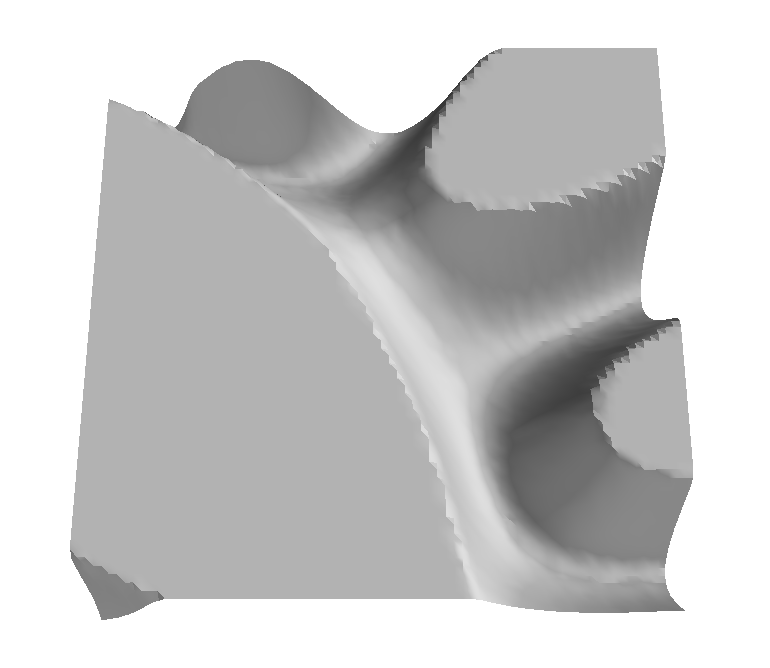
\includegraphics[width=\linewidth]{../img/5/train/all/03-patch-3d-majavi-7.png}
    \caption{$03$cm}
    \end{subfigure}
    \begin{subfigure}[b]{0.19\textwidth}
    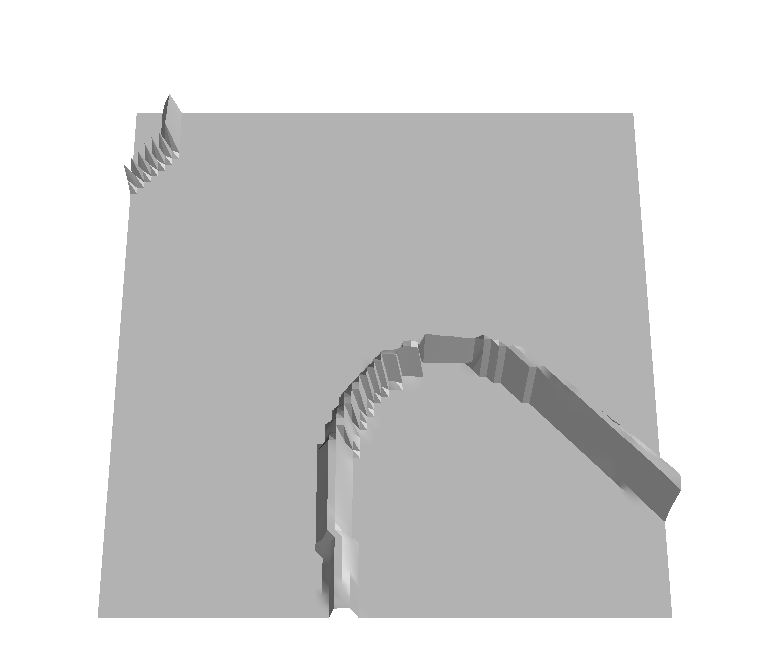
\includegraphics[width=\linewidth]{../img/5/train/all/05-patch-3d-majavi-8.png}
    \caption{$05$cm}
    \end{subfigure}
    \begin{subfigure}[b]{0.19\textwidth}
    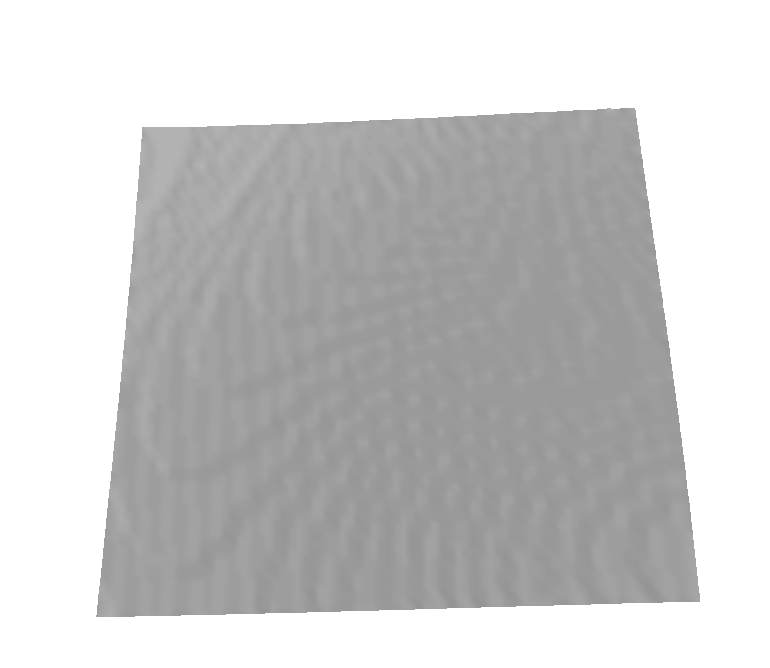
\includegraphics[width=\linewidth]{../img/5/train/all/08-patch-3d-majavi-9.png}
    \caption{$08$cm}
    \end{subfigure}
    \begin{subfigure}[b]{0.19\textwidth}
    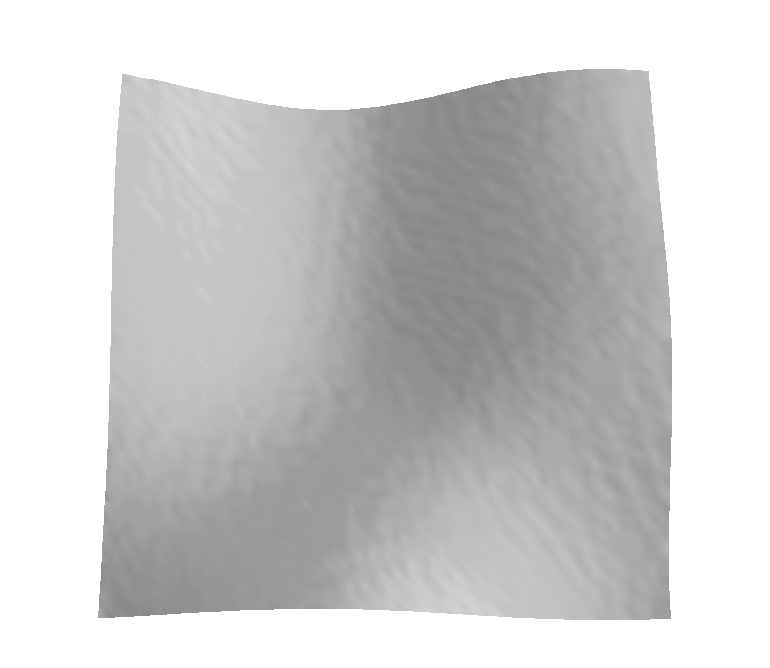
\includegraphics[width=\linewidth]{../img/5/train/all/11-patch-3d-majavi-10.png}
    \caption{$11$cm}
    \end{subfigure}
    \begin{subfigure}[b]{0.19\textwidth}
    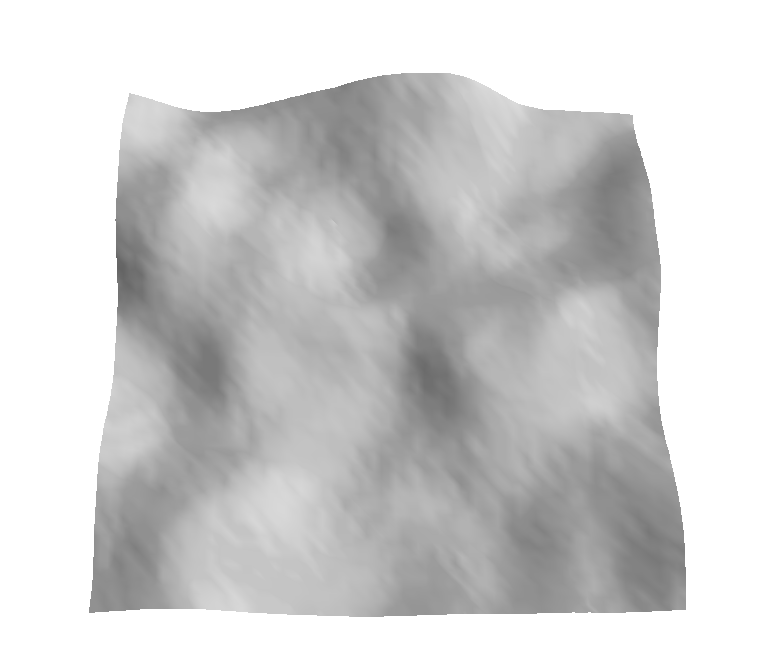
\includegraphics[width=\linewidth]{../img/5/train/all/14-patch-3d-majavi-11.png}
    \caption{$14$cm}
    \end{subfigure}
    \begin{subfigure}[b]{0.19\textwidth}
    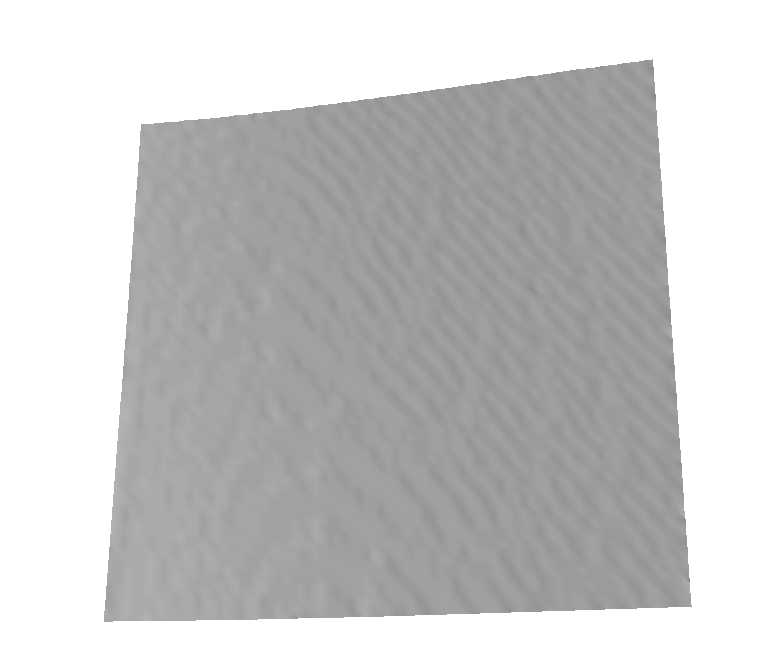
\includegraphics[width=\linewidth]{../img/5/train/all/17-patch-3d-majavi-12.png}
    \caption{$17$cm}
    \end{subfigure}
    \begin{subfigure}[b]{0.19\textwidth}
    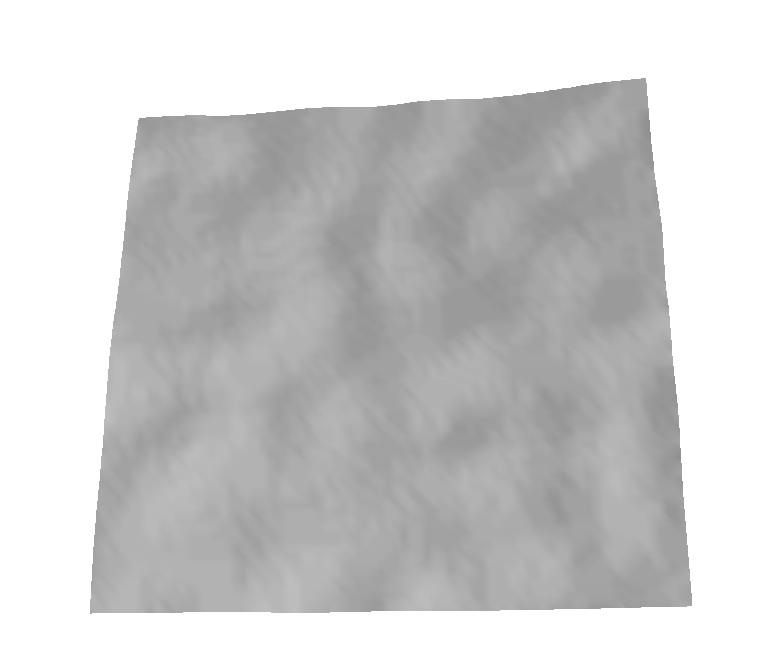
\includegraphics[width=\linewidth]{../img/5/train/all/20-patch-3d-majavi-13.png}
    \caption{$20$cm}
    \end{subfigure}
    \begin{subfigure}[b]{0.19\textwidth}
    \includegraphics[width=\linewidth]{../img/5/train/all/23-patch-3d-majavi-14.png}
    \caption{$23$cm}
    \end{subfigure}
    \begin{subfigure}[b]{0.19\textwidth}
    \includegraphics[width=\linewidth]{../img/5/train/all/26-patch-3d-majavi-15.png}
    \caption{$26$cm}
    \end{subfigure}
    \begin{subfigure}[b]{0.19\textwidth}
    \includegraphics[width=\linewidth]{../img/5/train/all/30-patch-3d-majavi-16.png}
    \caption{$30$cm}
    \end{subfigure}
    \begin{subfigure}[b]{0.19\textwidth}
    \includegraphics[width=\linewidth]{../img/5/train/all/33-patch-3d-majavi-17.png}
    \caption{$33$cm}
    \end{subfigure}
    \begin{subfigure}[b]{0.19\textwidth}
    \includegraphics[width=\linewidth]{../img/5/train/all/35-patch-3d-majavi-18.png}
    \caption{$35$cm}
    \end{subfigure}
    \begin{subfigure}[b]{0.19\textwidth}
    \includegraphics[width=\linewidth]{../img/5/train/all/38-patch-3d-majavi-19.png}
    \caption{$38$cm}
    \end{subfigure}
    \begin{subfigure}[b]{0.19\textwidth}
    \includegraphics[width=\linewidth]{../img/5/train/all/40-patch-3d-majavi-20.png}
    \caption{$40$cm}
    \end{subfigure}
    \begin{subfigure}[b]{0.19\textwidth}
    \includegraphics[width=\linewidth]{../img/5/train/all/43-patch-3d-majavi-21.png}
    \caption{$43$cm}
    \end{subfigure}
    \begin{subfigure}[b]{0.19\textwidth}
    \includegraphics[width=\linewidth]{../img/5/train/all/45-patch-3d-majavi-22.png}
    \caption{$45$cm}
    \end{subfigure}
    \begin{subfigure}[b]{0.19\textwidth}
    \includegraphics[width=\linewidth]{../img/5/train/all/47-patch-3d-majavi-23.png}
    \caption{$47$cm}
    \end{subfigure}
    \begin{subfigure}[b]{0.19\textwidth}
    \includegraphics[width=\linewidth]{../img/5/train/all/49-patch-3d-majavi-24.png}
    \caption{$49$cm}
    \end{subfigure}
    \begin{subfigure}[b]{0.19\textwidth}
    \includegraphics[width=\linewidth]{../img/5/train/all/51-patch-3d-majavi-25.png}
    \caption{$51$cm}
    \end{subfigure}
    \begin{subfigure}[b]{0.19\textwidth}
    \includegraphics[width=\linewidth]{../img/5/train/all/53-patch-3d-majavi-26.png}
    \caption{$53$cm}
    \end{subfigure}
    \begin{subfigure}[b]{0.19\textwidth}
    \includegraphics[width=\linewidth]{../img/5/train/all/54-patch-3d-majavi-27.png}
    \caption{$54$cm}
    \end{subfigure}
    \begin{subfigure}[b]{0.19\textwidth}
    \includegraphics[width=\linewidth]{../img/5/train/all/56-patch-3d-majavi-28.png}
    \caption{$56$cm}
    \end{subfigure}
    \begin{subfigure}[b]{0.19\textwidth}
    \includegraphics[width=\linewidth]{../img/5/train/all/57-patch-3d-majavi-29.png}
    \caption{$57$cm}
    \end{subfigure}
    \begin{subfigure}[b]{0.19\textwidth}
    \includegraphics[width=\linewidth]{../img/5/train/all/59-patch-3d-majavi-30.png}
    \caption{$59$cm}
    \end{subfigure}
    \begin{subfigure}[b]{0.19\textwidth}
    \includegraphics[width=\linewidth]{../img/5/train/all/60-patch-3d-majavi-31.png}
    \caption{$60$cm}
    \end{subfigure}
    \begin{subfigure}[b]{0.19\textwidth}
    \includegraphics[width=\linewidth]{../img/5/train/all/62-patch-3d-majavi-32.png}
    \caption{$62$cm}
    \end{subfigure}
    \begin{subfigure}[b]{0.19\textwidth}
    \includegraphics[width=\linewidth]{../img/5/train/all/63-patch-3d-majavi-33.png}
    \caption{$63$cm}
    \end{subfigure}
    \begin{subfigure}[b]{0.19\textwidth}
    \includegraphics[width=\linewidth]{../img/5/train/all/65-patch-3d-majavi-34.png}
    \caption{$65$cm}
    \end{subfigure}
    \begin{subfigure}[b]{0.19\textwidth}
    \includegraphics[width=\linewidth]{../img/5/train/all/66-patch-3d-majavi-35.png}
    \caption{$66$cm}
    \end{subfigure}
    \begin{subfigure}[b]{0.19\textwidth}
    \includegraphics[width=\linewidth]{../img/5/train/all/67-patch-3d-majavi-36.png}
    \caption{$67$cm}
    \end{subfigure}
    \begin{subfigure}[b]{0.19\textwidth}
    \includegraphics[width=\linewidth]{../img/5/train/all/69-patch-3d-majavi-37.png}
    \caption{$69$cm}
    \end{subfigure}
    \begin{subfigure}[b]{0.19\textwidth}
    \includegraphics[width=\linewidth]{../img/5/train/all/70-patch-3d-majavi-38.png}
    \caption{$70$cm}
    \end{subfigure}
    \begin{subfigure}[b]{0.19\textwidth}
    \includegraphics[width=\linewidth]{../img/5/train/all/73-patch-3d-majavi-39.png}
    \caption{$73$cm}
    \end{subfigure}
    \caption{Sample of extracted patches from the train set ordered by advancement. The first patches have mostly obstacle close to the robot's head, while the latter have smooter surfaces.}
    \label{fig : train-patches-sample}
    \end{figure}

\section{Label patches}
To classify the patches we first need to label them. We defined a thresold to represent and label each patch traversable if the advancement is greater or not traversle it is lower. Ideally, the threshold should small enough to include as less as possible false positive and big enough to cover all the cases where Krock gets stuck. We empirically compute the threshold's value by spawing Krock in front of a bumps and a ramp and let it walk.
    \paragraph{Bumps} We spawned the robot on the \emph{bumps3} map close to the end and let it go for 20 seconds. Figure \ref{fig : krock-bumps-sim} shows Krock in the simulated environment.
    
    \begin{figure}[htbp]
    \centering
        \begin{subfigure}[b]{0.45\textwidth}
        \includegraphics[width=\linewidth]{../img/3/find_tr/krock-bumps.jpg}
        \end{subfigure}
    \caption{Krock tries to overcome an obstacle in the \emph{bumps3} map.}
    \label{fig : krock-bumps-sim}
    \end{figure}
    Due to its characteristic locomotion, Krock tried to overcome the obstacle using its legs to move itself to the top but it fell backs producing a spicky advancement where first it is positive and then negative. Figure \ref{fig : krock-bumps-advs} shows the advancemnet on this map with $\Delta t = 2$, we can notice the noisy output.
    
    \begin{figure}[htbp]
        \centering
        \begin{subfigure}[b]{0.45\textwidth}
            \includegraphics[width=\linewidth]{../img/3/find_tr/100-bumps3}
        \end{subfigure}
    
    \caption{Advancement over time with  $\Delta t = 2$ on \emph{bumps3}.}
    \label{fig : krock-bumps-advs}
    \end{figure}
    A wheel robot, on the other hand, will not produce such graph since it cannot free itself easily from an obstacle. Image a wheel robot moving forward, once it hits an obstance it stops moving, if we plot its advancement in this situation it will look more like a step than a series of spikes.
    \paragraph{Ramps}
    The trehsold should be small enough to not create any false positive, patches that are traversable but were classified as not. So, we let the robot walk up hill on the $slope_rocks1$ map with a height scaling factor set to $5$. We knew from empirical experiment that the robot is able to climp this steep ramp, the advancement is showed in figure \ref{fig : krock-ramps-sim}.
    \begin{figure}[htbp]
        \centering
        \begin{subfigure}[b]{0.45\textwidth}
            \includegraphics[width=\linewidth]{../img/3/find_tr/100-slope_rocks1}
        \end{subfigure}
        \caption{Advancement over time with $\Delta t = 2$s on \emph{slope\_rocks3}.}
        \label{fig : krock-ramps-sim}
    \end{figure}
    The mean $\approx 0.4$cm over a $\Delta t =2$, an impressive value considering the steepest of the surface. We used this information combined with the previous experiment to choose a threshold that is beetween the upper bound of \emph{bumps} and beetween the lower bound of \emph{slope\_rocks1}. This ensured to minimize the false positive. A good value is $tr_{\Delta t = 2s} = 20cm$. 
\section{Estimator}
\label{sec: estimator}
In this section we described  the five convolution neural networks architecture we tested.
\subsection{Vanilla Model}
\label{subsec : vanilla-cnn}

The original model proposed by Chavez-Garcia et all \cite{omar2018traversability} is a CNN composed by a two $3 \times 3$ convolution layer with $5$ filters; $2 \times 2$ Max-Pooling layer; $3 \times 3$ convolution layer with $5$ filters; a fully connected layer with 128 outputs neurons and a fully connected layers with two neurons. Figure \ref{fig : omar} visualizes the architecture. 

\begin{figure}[htbp]
    \centering
    \begin{subfigure}[b]{0.25\linewidth}
        \includegraphics[width=\linewidth]{../img/3/models/transparent-omar.png}
    \end{subfigure}
    \caption{Vanilla model proposed by Chavez-Garcia et al. \cite{omar2018traversability}. The rectangle represent the building block of each layer. Convolutiol layers are described by the kernel size, the number of filters and the stride.}
    \label{fig : omar}
\end{figure}
\subsection{ResNet}
We adopt a Residual Network, ResNet \cite{he2015deep}, variant. Residual networks are deep convolutional networks consisting of many stacked \" Residual Units \". Intuitively, the residual unit allows the input of a layer to contribute to the next layer's input by being added to the current layer's output. Due to possible different features dimension, the input must go through and identify map to make the addition possible. This allows a stronger gradient flows and mitigates the degradation problem. A \"Residual Units \" is composed by a two $3x3$ \emph{Convolution}, \emph{Batchnorm} \cite{ioffe2015batch} and a \emph{Relu} blocks. Formally defined as: 
\begin{equation}
    \mathbf{y}=\mathcal{F}\left(\mathbf{x},\left\{W_{i}\right\}\right)+h(\mathbf{x})
    \label{eq : resnet}
\end{equation}
Where, $x$ and $y$ are the input and output vector of the layers considered. The function $\mathcal{F}\left(\mathbf{x},\left\{W_{i}\right\}\right)$ is the residual mapping to be learn and $h$ is the identity mapping. The next figure visualises the equation.
\begin{figure}[htbp]
    \centering
    \includegraphics[scale=0.3]{../img/implementation/estimator/resnet_block.png}
    \caption{\emph{Resnet} block \cite{he2015deep}}
\end{figure}
When the input and output shapes mistmatch, the \emph{identity map} is applyed to the input as a $3x3$ Convolution with a stride of 2 to mimic the polling operator. A single block is composed by a $3x3$ \emph{Convolution}, \emph{Batchnorm} and a \emph{Relu} activation function. 
\subsection{Preactivation}
Following the recent work of He et al. \cite{he2015identity} we adopted \emph{pre-activation} in each block.\emph{Pre-activation} works by just reversing the order of the operations in a block.

\begin{figure}[htbp]
    \centering
    \includegraphics[scale=0.2]{../img/implementation/estimator/preactivation.png}
    \caption{\emph{Preactivation} \cite{he2015identity}}
\end{figure}
\subsection{Sqeeze and Excitation}
Finally, we also used the \emph{Squeeze and Excitation} (SE) module \cite{hu2017squeeze}. It is a form of attention that weights the channel of each convolutional operation by learnable scaling factors. Formally, for a given transformation, e.g. Convolution, defined as $\bm{F}_{tr}  : \bm{X} \mapsto \bm{U}$, $\bm{X} \in mathbb{R}^{H' \times W' \times C'}$, $\bm{U} \in \mathbb{R}^{H \times W \times C}$, the SE module first squeeze the information by using average pooling, $\bm{F}_{sq}$, the it excitates them using learnable weights, $\bm{F}_{ex}$ and finally, adaptive recalibration is performed, $\bm{F}_{scale}$.
The next figure visualises the SE module.

\begin{figure}[htbp]
    \centering
    \includegraphics[width=\linewidth]{../img/implementation/estimator/se.png}
    \caption{\emph{Squeeze and Excitation} \cite{hu2017squeeze}}
\end{figure}
\subsection{MicroResNet}
\label{subsec : micro-resnets}
The proposed network's architecture is composed by $n$ ResNet blocks and channel incrementing factor of $2$. Originally, ResNet was used to classify RGB images with $224\times224$ pixels and  used an aggressive convolution and max-polling operation in the first layer to reduce the images's size. We decided to adopt a less aggressive convolution motivited by the smaller size of our inputs. We tested two kernel sized: $7\times7$ and $3\times3$ with stride of $2$ and $1$ respectively. Lastly, we used LeakyReLU \cite{leakyrelu} with a negative slope of $0.1$ instead of ReLU to allow a better gradient flow during backpropagation. LeakyRelu is defined as follows
\begin{equation}
LeakyRelu(x)=\left\{\begin{array}{ll}{x} & {\text { if } x>0} \\ {0.1 x} & {\text { otherwise }}\end{array}\right.
\end{equation}

We called this model architecture \emph{MicroResNet}. We proposed four networks layouts: with $n=1$ and two fist layers setups, $3\times3$ stride $=1$ and $7\times7$, with and without the Squeeze and Excitation module. Those architectures can be used both for regression and classification by only chaning the output size of the fully connected later, $2$ for classification and $1$ for regression. All others layers are equals. Figure \ref{fig : microresnet} add additional informations.
\begin{table}[htbp]
    \centering
    \ra{1.2}
        \begin{tabular}{@{}l|c|c|c|cc@{}}
        \hline
             Input   &  \multicolumn{4}{c}{$(1,78,78)$}  \\ 
            \hline 
            \multirow{12}{*}{Layers} & \multicolumn{2}{c}{$3 \times 3$, $16$ stride $1$} & \multicolumn{2}{c}{$7 \times 7$ $16$ stride $2$} \\
            \cline{2-5}
            &\multicolumn{4}{c}{$2 \times \ 2$ max-pool} \\ 
            \cline{2-5}
            &  \multicolumn{4}{c}{$\begin{bmatrix}
                3  \times 3, & 16 \\
                3  \times  3, & 32 \\  
               \end{bmatrix}$ x 1} \\ 
               \cline{2-5}
               &  SE & - & SE & -\\ 
               \cline{2-5}
               &  \multicolumn{4}{c}{$\begin{bmatrix}
                3  \times 3, & 32 \\
                3  \times  3, & 64 \\  
               \end{bmatrix}$ x 1} \\ 
               \cline{2-5}
               &  SE & - & SE & -\\ 
               \cline{2-5}

               &  \multicolumn{4}{c}{$\begin{bmatrix}
                3  \times 3, & 64 \\
                3  \times  3, & 128 \\  
               \end{bmatrix}$ x 1} \\
               \hline
               &  SE & - & SE & -\\ 
               \cline{2-5}
               &  \multicolumn{4}{c}{average pool, $1$-d fc, softmax} \\ 
               \hline
        
               Parameters &  313,642 & 302,610  &  314,28 & 303,250 \\
            \hline
               Size (MB) & 5.93 & 5.71 &  2.41 & 2.32 \\ 
               \hline 
        \end{tabular}
        \caption{MicroResNet architecture. First layer is on the top. Some architecture's blocks are equal across models, this is shows by sharing columns in the table.}
        \ref{tab : microresnet}
    \end{table}
Our models have approximately $35$ times less parameters than the smalles ResNet model, ResNet18 \cite{he2015deep}, that has $11$M parameters. To simplicity we used the following notation to describe each architecture variant: \texttt{MicroResNet-{3x3/7x7}-{/SE}}.
\begin{figure}[htbp]
    \centering
    \begin{subfigure}[b]{0.22\textwidth}
        \includegraphics[width=\textwidth]{../img/3/models/transparent-microresnet3x3.png}
        \caption{}
    \end{subfigure}
    \begin{subfigure}[b]{0.22\textwidth}
        \includegraphics[width=\textwidth]{../img/3/models/transparent-microresnet3x3-se.png}
        \caption{}
    \end{subfigure} 
    \begin{subfigure}[b]{0.22\textwidth}
        \includegraphics[width=\textwidth]{../img/3/models/transparent-microresnet7x7.png}
        \caption{}
    \end{subfigure}
    \begin{subfigure}[b]{0.22\textwidth}
        \includegraphics[width=\textwidth]{../img/3/models/transparent-microresnet7x7-se.png}
        \caption{}
    \end{subfigure} 
    \caption{MicroResNet architectures for classification. All models have an initial features size of $16$ and $n=1$ with and without the Squeeze and Excitation module. The rectangle represent the building block of each layer. Convolutiol layers are described by the kernel size, the number of filters and the stride. Lines and dashed lines between layers represent the residual operations and the shortcut respectively.}
    \label{fig : microresnet}
\end{figure}

\section{Normalization}
Before feeding the data to the models, we need to make the patches height invariant to correctly normalize different patches taken from different maps with different height scaling factor. To do so, we subtract the height of the map corresponding \emph{Krock}'s position from the patch to correctly center it. The following figure shows the normalization process on the patch with the square in the middle.
\begin{figure}[htbp]
    \centering
    \begin{subfigure}[b]{0.32\textwidth}
        \includegraphics[width=\textwidth]{../img/data-aug/2d/square-middle.png}
        \caption{Input}
    \end{subfigure}
    \begin{subfigure}[b]{0.32\textwidth}
        \includegraphics[width=\textwidth]{../img/data-aug/2d/square-middle-center.png}
        \caption{Height centered}
    \end{subfigure}  
    \\
          \begin{subfigure}[b]{0.32\textwidth}
        \includegraphics[width=\textwidth]{../img/data-aug/3d/square-middle.png}
        \caption{Input}
    \end{subfigure}
    \begin{subfigure}[b]{0.32\textwidth}
        \includegraphics[width=\textwidth]{../img/data-aug/3d/square-middle-center.png}
        \caption{Height centered}
    \end{subfigure}  
\caption{Normalization process. Each patch is normalized by subtracting the height value corresponding to the robot position to center its height. }
\label{fig: center}
\end{figure}

\section{Data Augmentation}
\label{sec: data-aug}
Data augmentation is used to change the input of a model in order to produce more training examples. Since our inputs are heightmaps we cannot utilize the classic image manipulations such as shifts, flips, and zooms. Imagine that we have a patch with a wall in front of it, if we random rotate the image the wall may go in a position where the wall is not facing the robot anymore, making the image now traversable with a wrong target. We decided to apply dropout, coarse dropout, and random simplex noise since they are traversability invariant. To illustrate those techniques we are going to use the same square patch showed before \ref{fig: center}.

\subsection{Dropout}
Dropout is a technique to randomly set some pixels to zero, in our case we flat some random pixel in the patch. 
\subsection{Coarse Dropout}
Similar to dropout, it sets to zero random regions of pixels with defined boundaries. 
\subsection{Simplex Noise} 
Simplex Noise is a form of Perlin noise that is mostly used in ground generation. Our idea is to add some noise to make the network generalize better since lots of training maps have only obstacles in flat ground. Since it is computationally expensive, we randomly fist apply the noise to five hundred images with only zeros. Then, we randomly scaled them and add to the input image. 
\begin{figure}[htbp]
    \centering

        \begin{subfigure}[b]{0.23\textwidth}
            \includegraphics[width=\textwidth]{../img/data-aug/3d/simplex1.png}
            \caption{Features size = 10}
        \end{subfigure}
        \begin{subfigure}[b]{0.23\linewidth}
            \includegraphics[width=\textwidth]{../img/data-aug/3d/simplex2.png}
            \caption{Features size = 20}
            \end{subfigure}    
          \begin{subfigure}[b]{0.23\textwidth}
            \includegraphics[width=\textwidth]{../img/data-aug/3d/simplex3.png}
            \caption{Features size = 30}
        \end{subfigure}    
        \begin{subfigure}[b]{0.23\textwidth}
            \includegraphics[width=\textwidth]{../img/data-aug/3d/simplex4.png}
            \caption{Features size = 40}
        \end{subfigure}    
    \caption{Simplex noise on flat ground. The feature size corespond to the amount of noise we introduce in the surface. A lower value produces noisy grounds, while a bigger one smoother terrains.}    
    \label{fig: simplex-noise}

\end{figure}

Figure \ref{fig: data-aug} shows the tree data augmentation techniques used applied the input image.
\begin{figure}[htbp]
    \centering
        \begin{subfigure}[b]{0.32\textwidth}
            \includegraphics[width=\textwidth]{../img/data-aug/3d/center-dropout-mayavi.png}
            \caption{Dropout}
        \end{subfigure}
        \begin{subfigure}[b]{0.32\linewidth}
            \includegraphics[width=\textwidth]{../img/data-aug/3d/center-coarse-dropout-mayavi.png}
            \caption{Coarse Dropout}
            \end{subfigure}    

          \begin{subfigure}[b]{0.32\textwidth}
            \includegraphics[width=\textwidth]{../img/data-aug/3d/center-simplex-mayavi.png}
            \caption{Simplex Noise}

        \end{subfigure}    
        \begin{subfigure}[b]{0.32\textwidth}f
            \includegraphics[width=\textwidth]{../img/data-aug/3d/center-final-mayavi.png}
            \caption{Final result}
        \end{subfigure}    
    \label{fig: data-aug}
    \caption{Data augmentation applied on a patch. First we randomly set to flat some small regions of the ground. Then, we slighty mutate the surface using simplex noise.}    
\end{figure}
To ensure we do create untraversable patches from traversable patch we limited the coarse dropout region to only few centiments and we apply a smoother simplex noise on traversable patches. In detail, in all the traning epochs, we augmented $80\%$ of the input images with dropout and coarse dropout. Dropout has a probability between $0.05$ and $0.1$ and coarse dropout has a probability of $0.02$ and $0.1$ with a size of the lower resolution image from which to sample the dropout between $0.6$ and $0.8$. Simplex noise was applied on the $70\%$ of the training data samples with a feature size between $1$ and $50$ with a random scaling factor between $15 - 25$ and $5 - 15$ from traversable and not traversable patches respectively. 

\section{Tools}
We quickly list the most important tools and libraries adopted in this project. The framework was entirely developed on Ubuntu 18.10 with Python 3.6.
\subsection{Software for simulation}
\paragraph{ROS Melodic} The Robot Operating System (ROS) \cite{ROS} is a flexible framework for writing robot software. It is \emph{de facto} the industry and research standard framework for robotics due to its simple yet effective interface that facilitates the task of creating a robust and complex robot behavior regardless of the platforms. ROS works by establishing a peer-to-peer connection where each \emph{node} is to communicate between the others by exposing sockets endpoints, called \emph{topics}, to stream data or send \emph{messages}. Each \emph{node} can subscribe to a \emph{topic} to receive or publish new messages. In our case, \emph{Krock} exposes different topics on which we can subscribe in order to get real-time information about the state of the robot.
Unfortunately, ROS does not natively support Python3, so we had to compile it by hand. Because it was a difficult and time-consuming operation, we decided to share the ready-to-go binaries as a \href{https://hub.docker.com/r/zuppif/ros-melodic-python3/}{docker image}. 

\subsection{Data processing}
\paragraph{Numpy}\href{https://www.numpy.org/}{Numpy} is a fundamental package for any scientific use. It allows to express efficiently any matrix operation using its broadcasting functions. Numpy is used across the whole pipeline to manipulate matrices.
\paragraph{Pandas}To process the data from the simulations we rely on \href{https://pandas.pydata.org/}{Pandas}, a Python library providing fast, flexible, and expressive data structures in a tabular form. Pandas is well suited for many different kinds of data such as handle tabular data with heterogeneously-typed columns, similar to SQL table or Excel spreadsheet, time series and matrices. We take advantages of the relationa data structure to perform custom manipulation on the rows by removing the outliears and computing the advancement.

Generally, pandas does not scale well and it is mostly used to handle small dataset while relegating \"big data\" to other frameworks such as Spark or Hadoop. We used Pandas to store the results from the simulator and inside a Thread Queue to parse each \emph{.csv} file efficiently.
\paragraph{OpenCV} Open Source Computer Vision Library, \href{https://opencv.org/}{OpenCV}, is an open source computer vision library with a rich collection of highly optimized algorithms. It includes classic and state-of-the-art computer vision and machine learning methods applied in a wide array of tasks, such as object detection and face recognition. We adopt this library to handle image data, mostly to pre and post-process the heightmaps and the patches.
\subsubsection{CNN training}
\paragraph{Pytorch }\href{https://pytorch.org/}{PyTorch} is a Python open source deep learning framework. It allows Tensor computation (like NumPy) with strong GPU acceleration and Deep neural networks built on a tape-based auto grad system. Due to its Python-first philosophy, it is easy to use, expressive and predictable it is widely used amoung researches and enthusiast. Moreover, its main advantages over other mainstream frameworks such as TensorFlow \cite{tensorflow} are a cleaner API structure, better debugging, code shareability and an enormous number of high-quality third-party packages.
\paragraph{FastAI}\href{https://course.fast.ai/}{FastAI} is library based on PyTorch that simplifies fast and accurate neural nets training using modern best practices. It provides a high-level API to train, evaluate and test deep learning models on any type of dataset. We used it to train, test, and evaluate our models.
\paragraph{imgaug}\href{https://imgaug.readthedocs.io/en/latest/}{Image augmentation} (imgaug) is a python library to perform image augmenting operations on images. It provides a variety of methodologies, such as affine transformations, perspective transformations, contrast changes and Gaussian noise, to build sophisticated pipelines. It supports images,  heatmaps, segmentation maps, masks, key points/landmarks, bounding boxes, polygons, and line strings. We used it to augment the heightmap, details are in \hyperref[sec: data-aug]{section \ref{sec: data-aug}}
\subsection{Visualization}
\paragraph{matplotlib}Almost all the plots in this report were created by \href{https://matplotlib.org/}{Matplotlib}, is a Python 2D plotting library. It provides a similar functional interface to MATLAB and a deep ability to customize every region of the figure. All 
It is worth citing \emph{seaborn} a data visualization library that we inglobate in our work-flow to create the heatmaps. It is based on Matplotlib and it provides an high-level interface.
\paragraph{mayavi}Mayavi is a scientific data visualization and plotting in python library. We adopt it to rendered in 3D all the surfaces used in our framework.

\end{document}